\section{Figure}
\subsection{Overview}
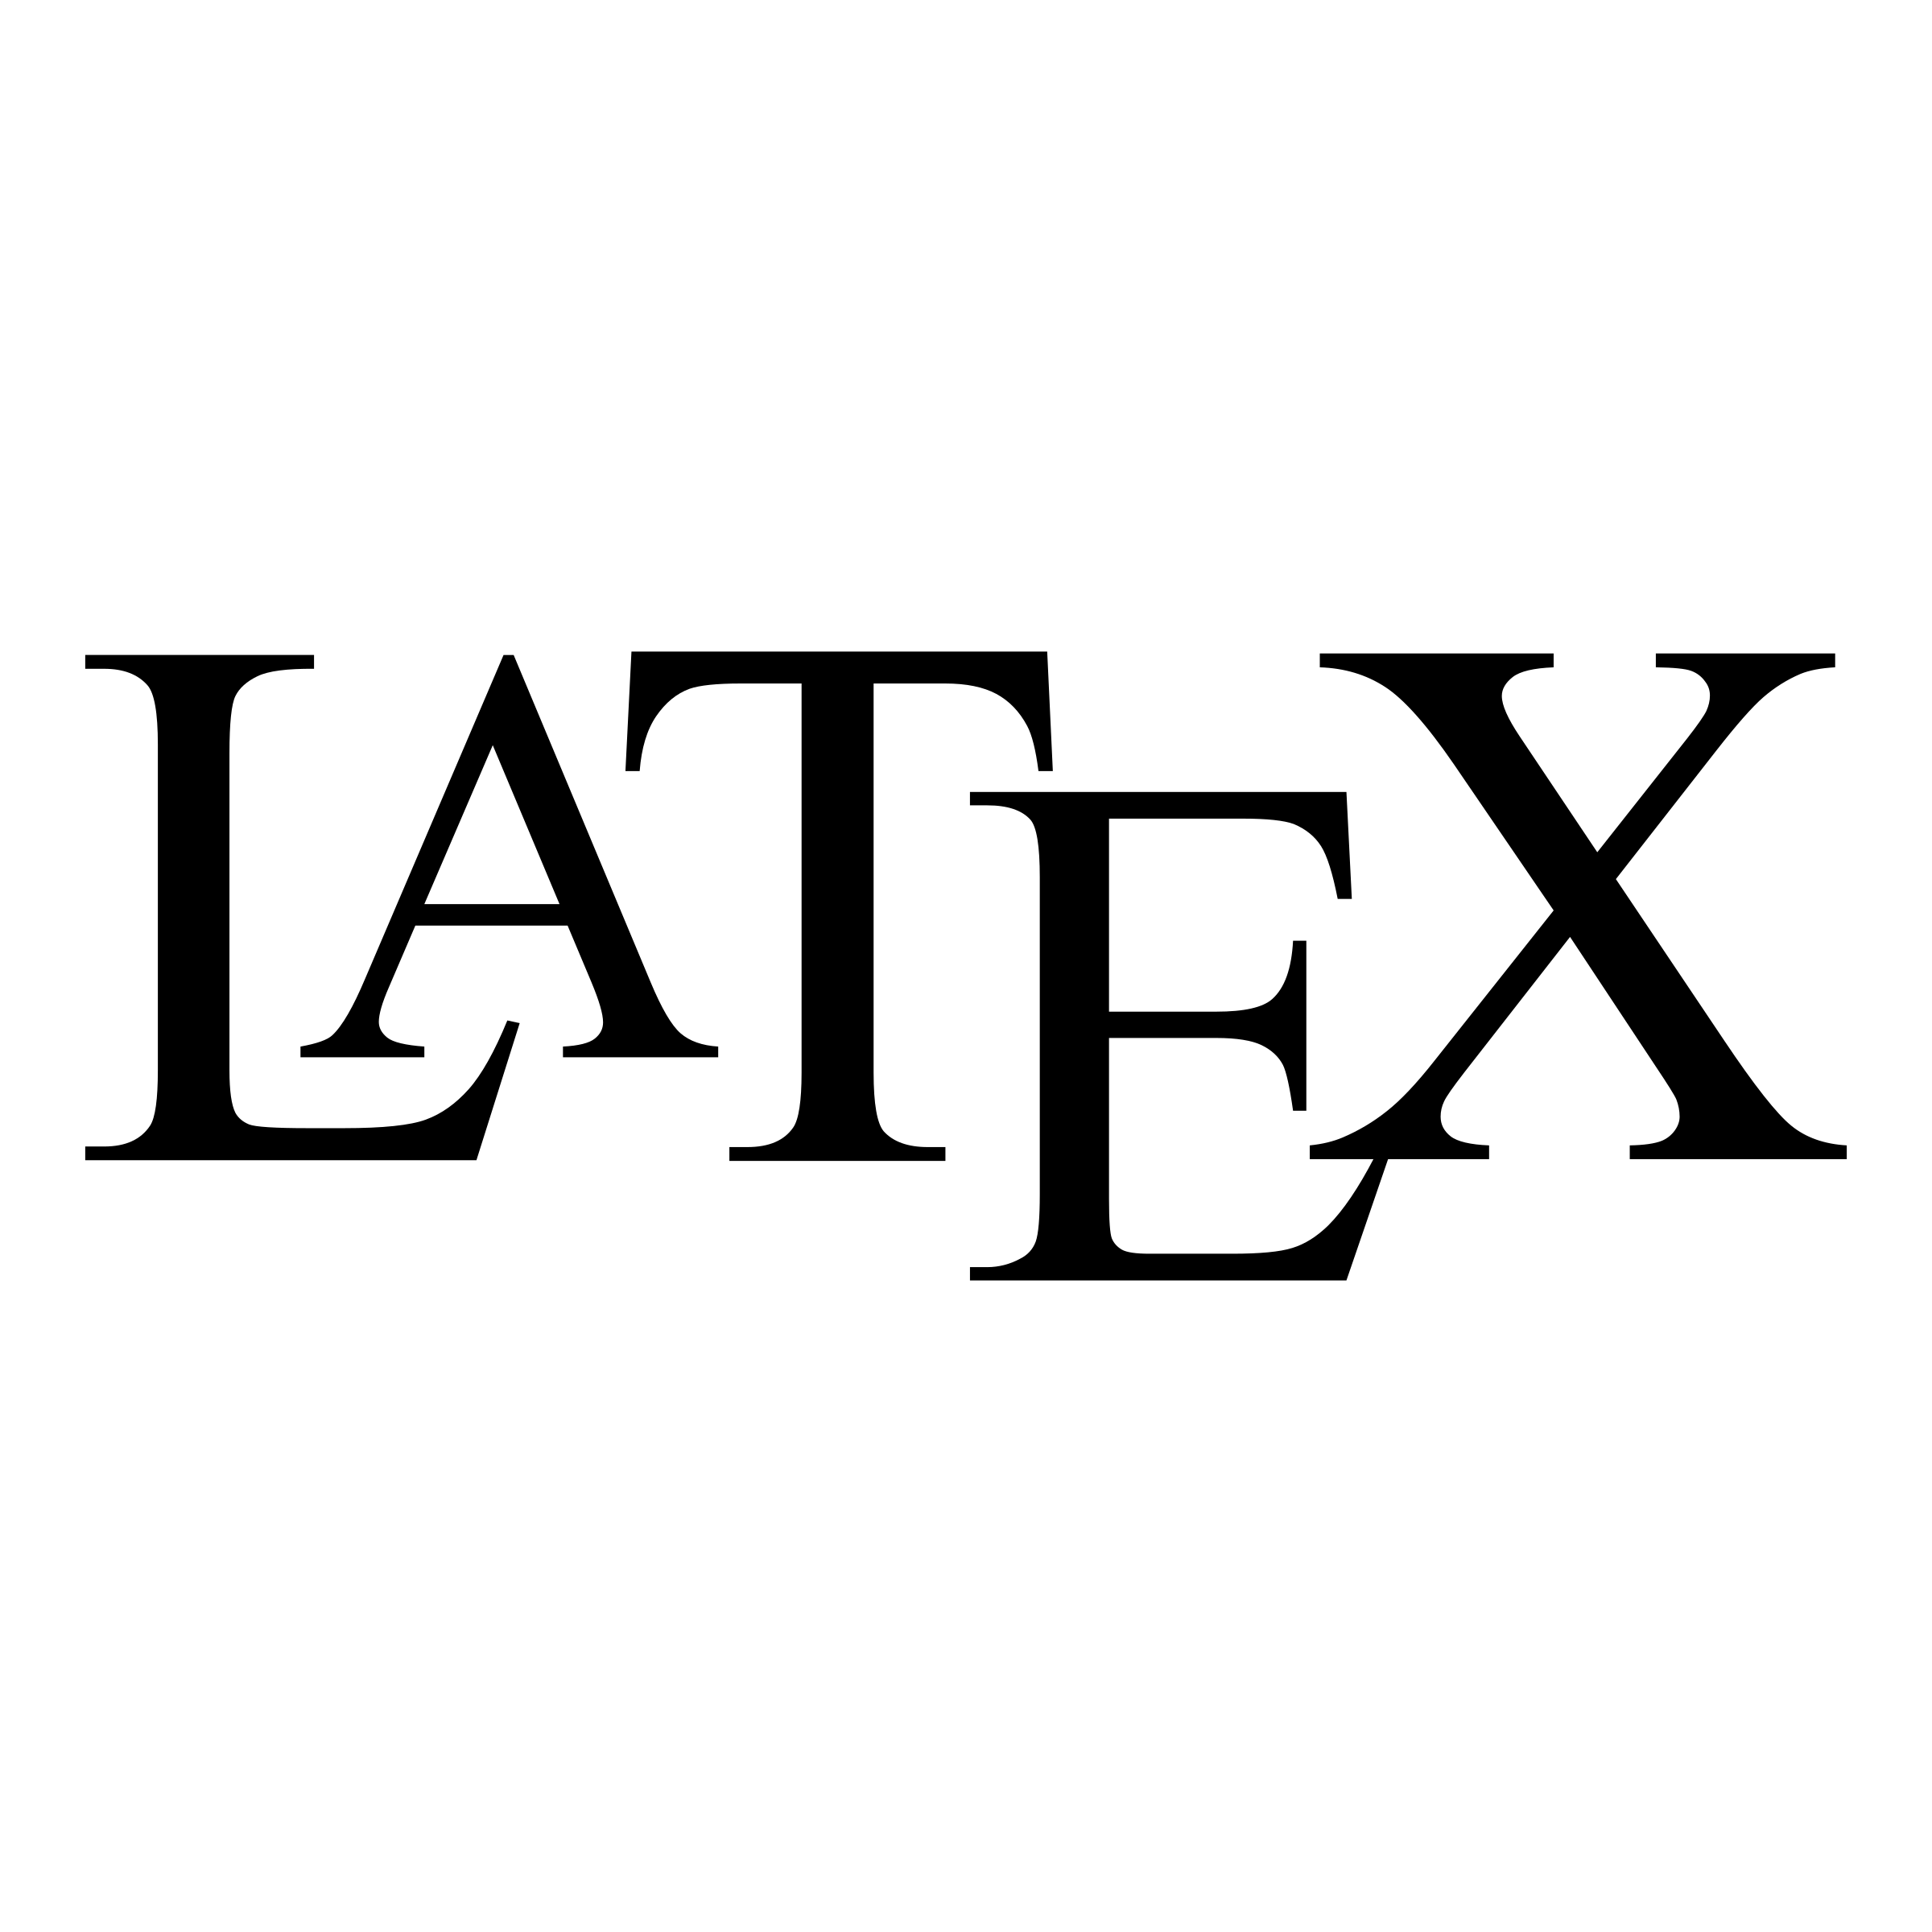
\includegraphics[scale=0.02]{LatexLogo.png}
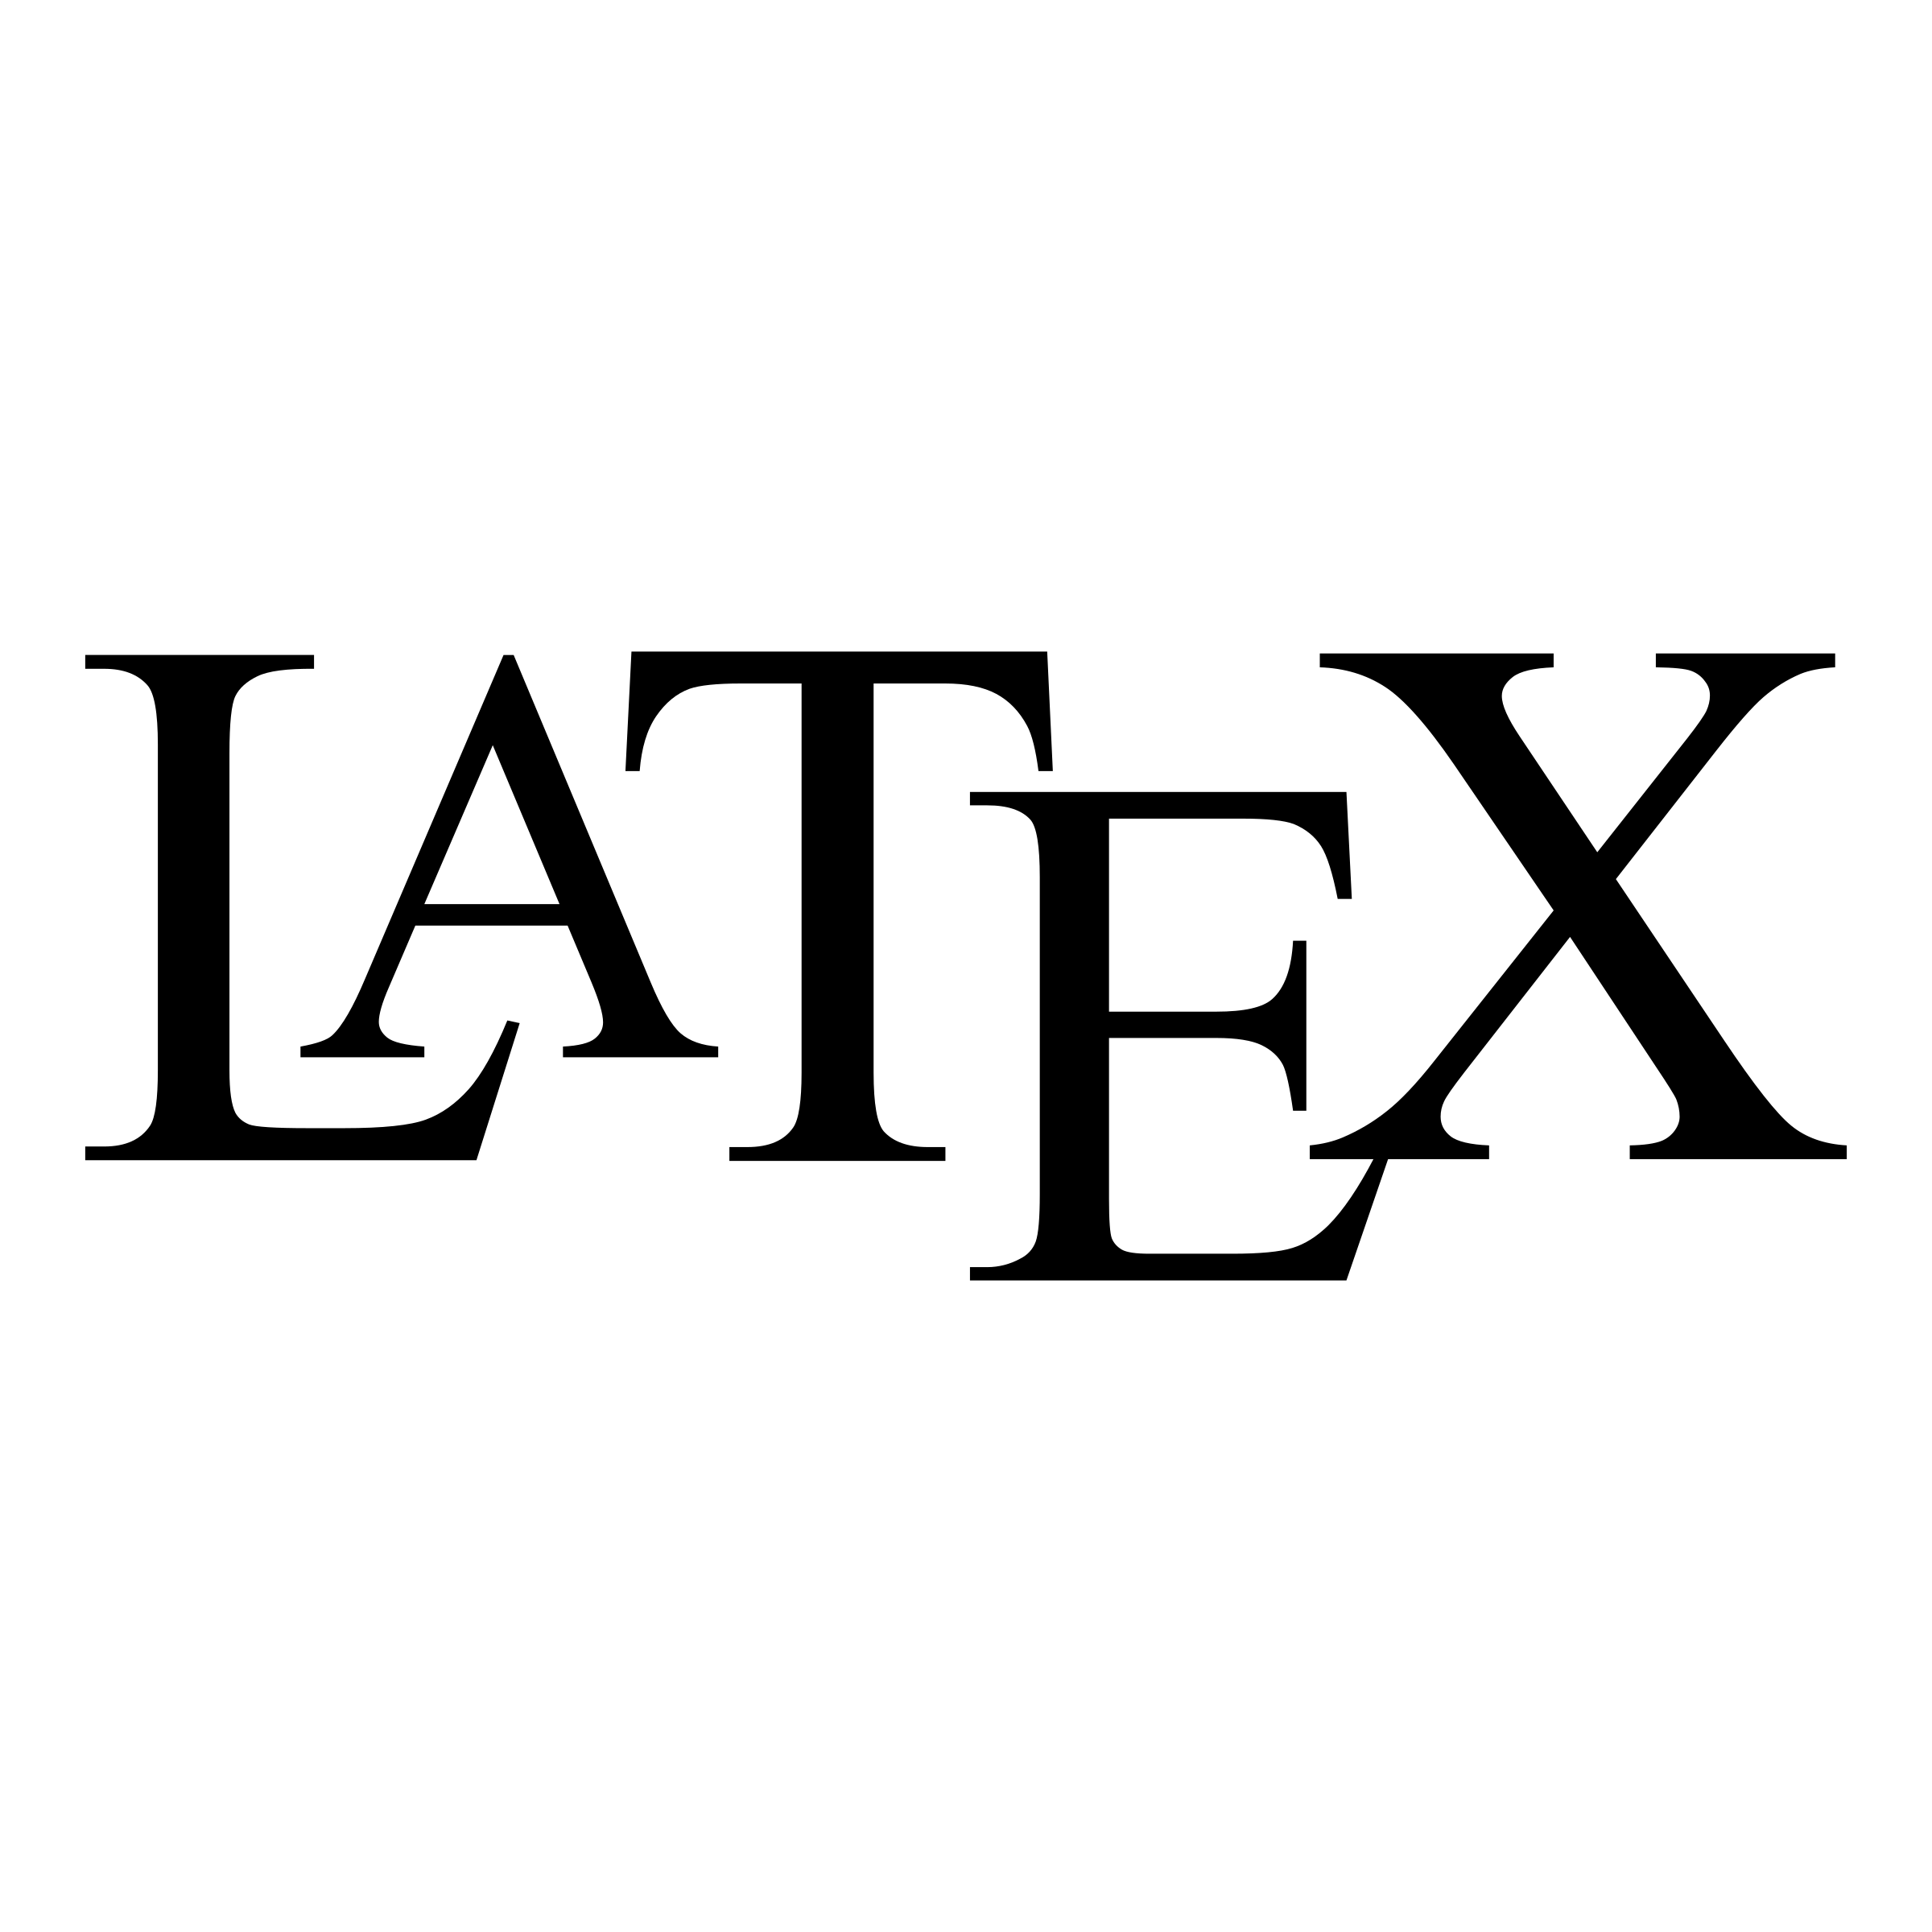
\includegraphics[width=2cm]{LatexLogo.png}
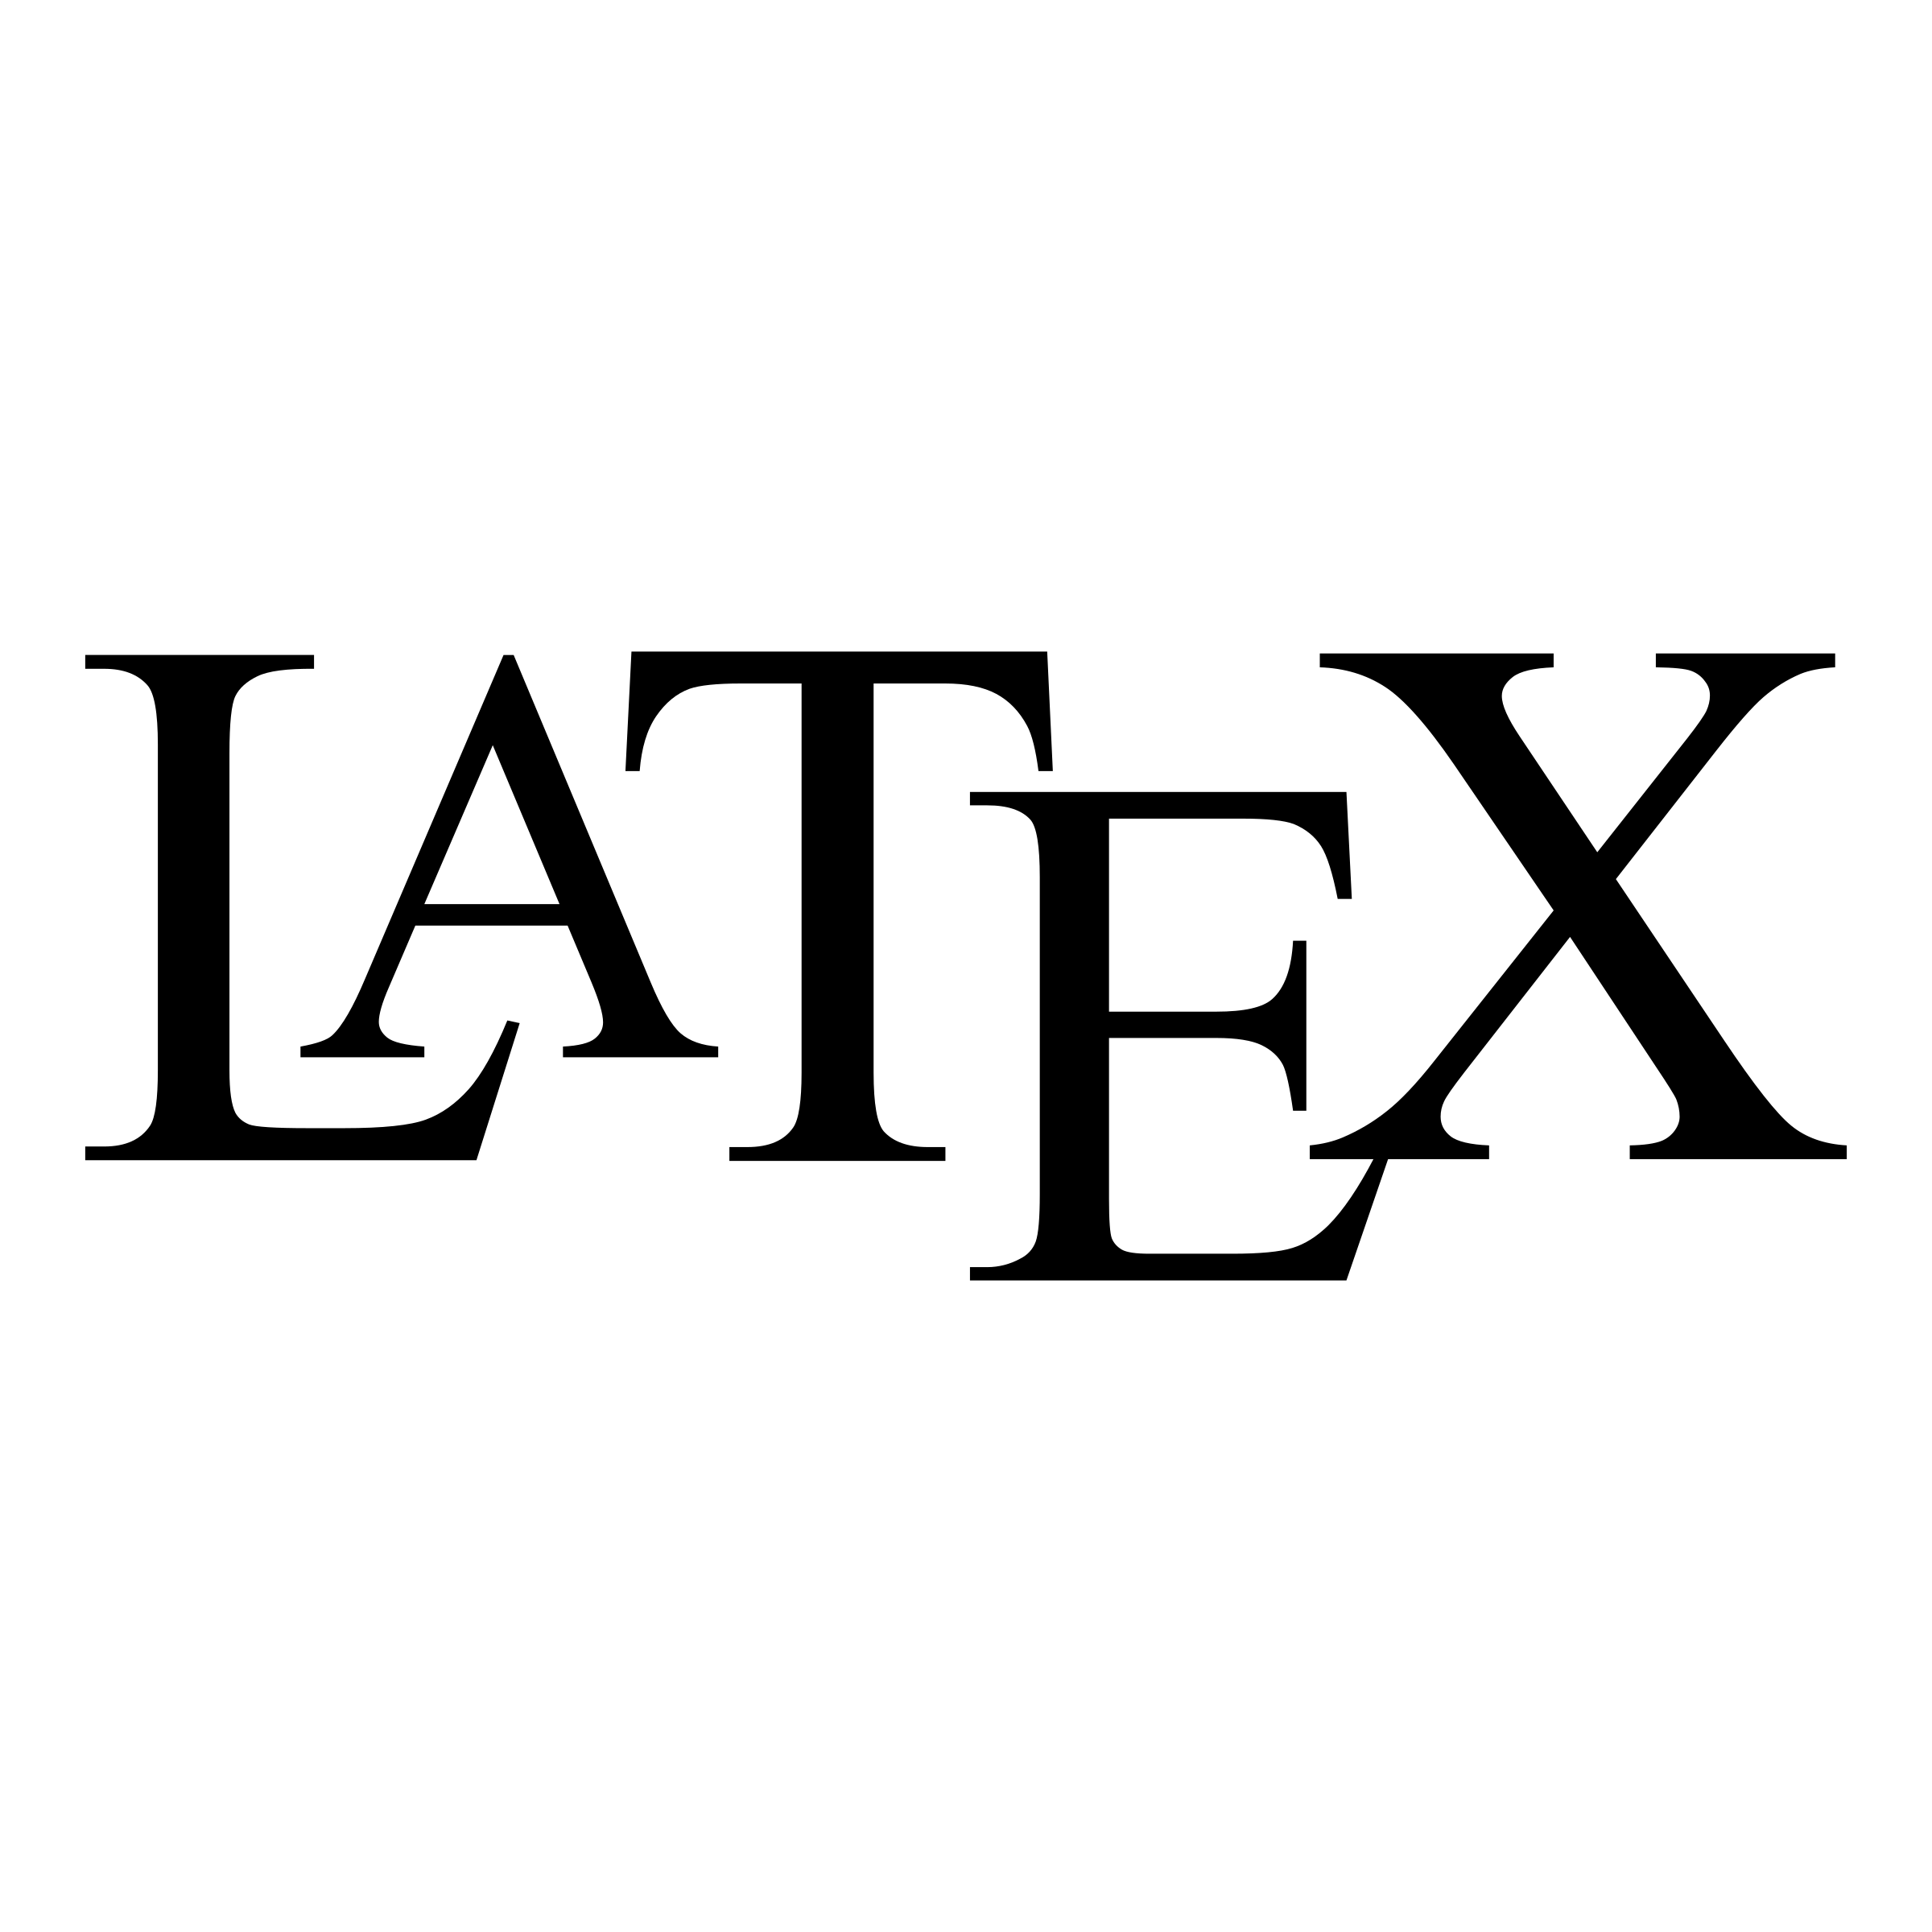
\includegraphics[height=2cm]{LatexLogo.png}
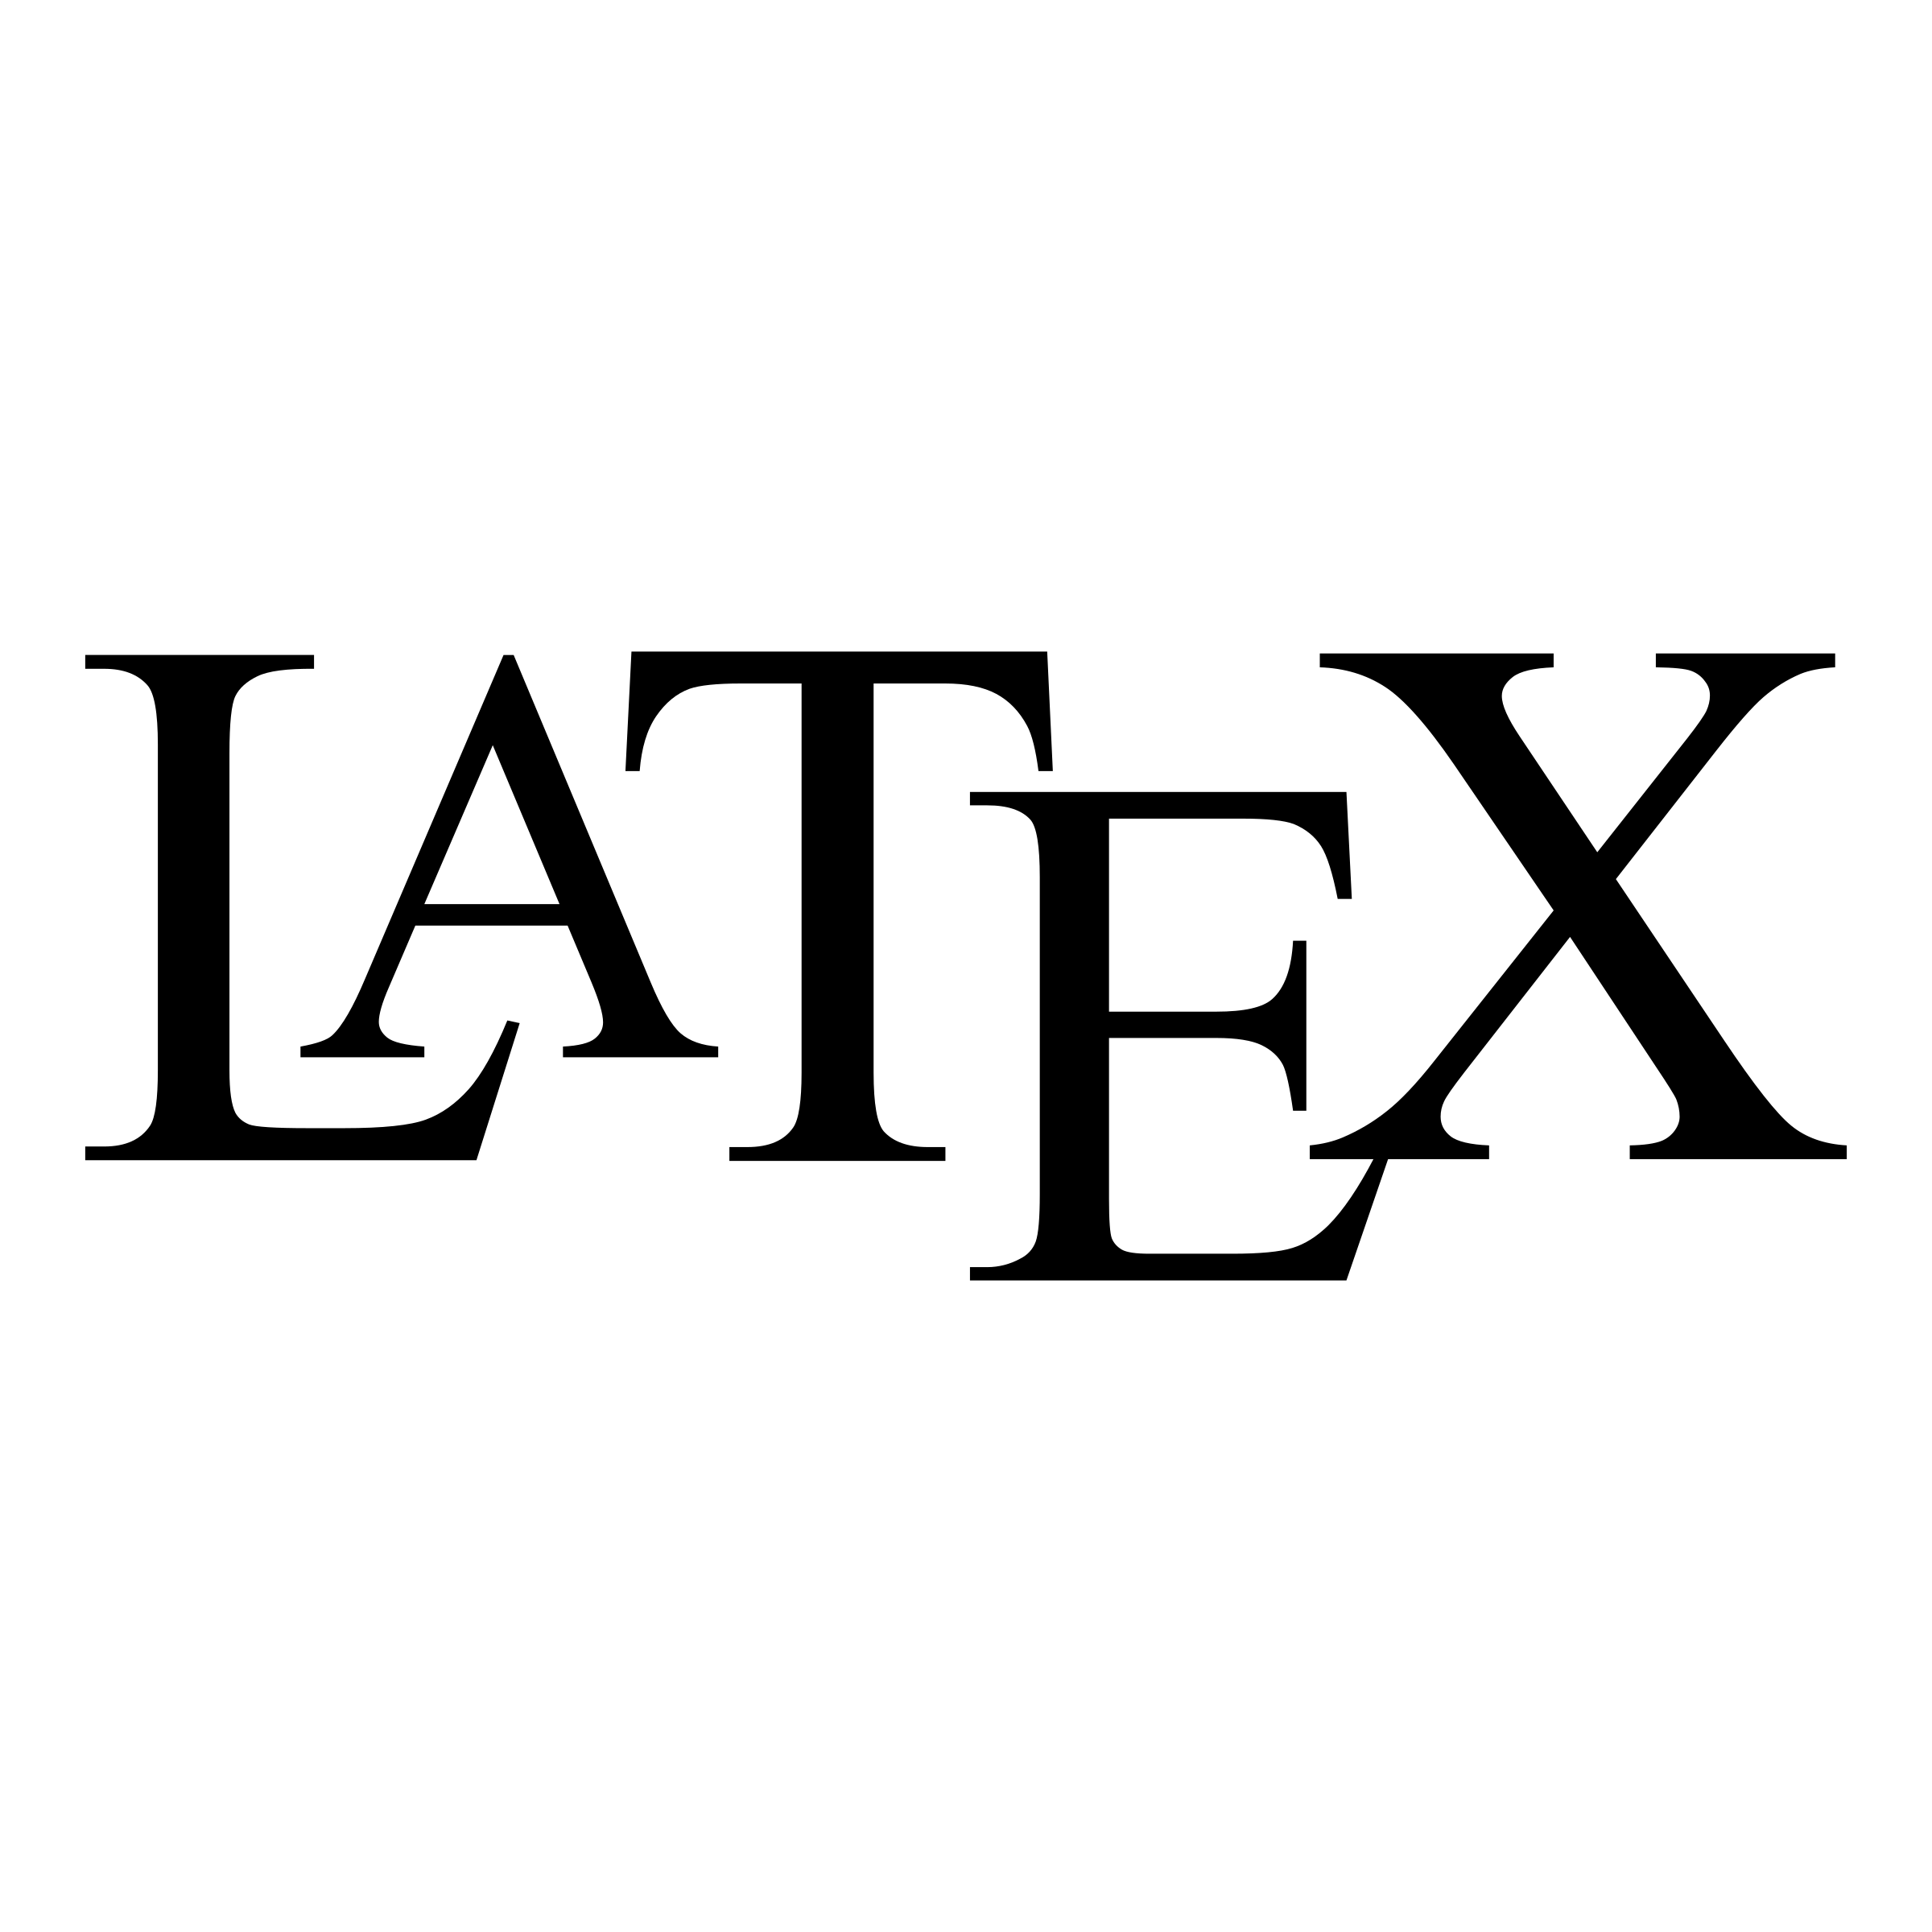
\includegraphics[angle=90, origin=c, scale=0.02]{LatexLogo.png}
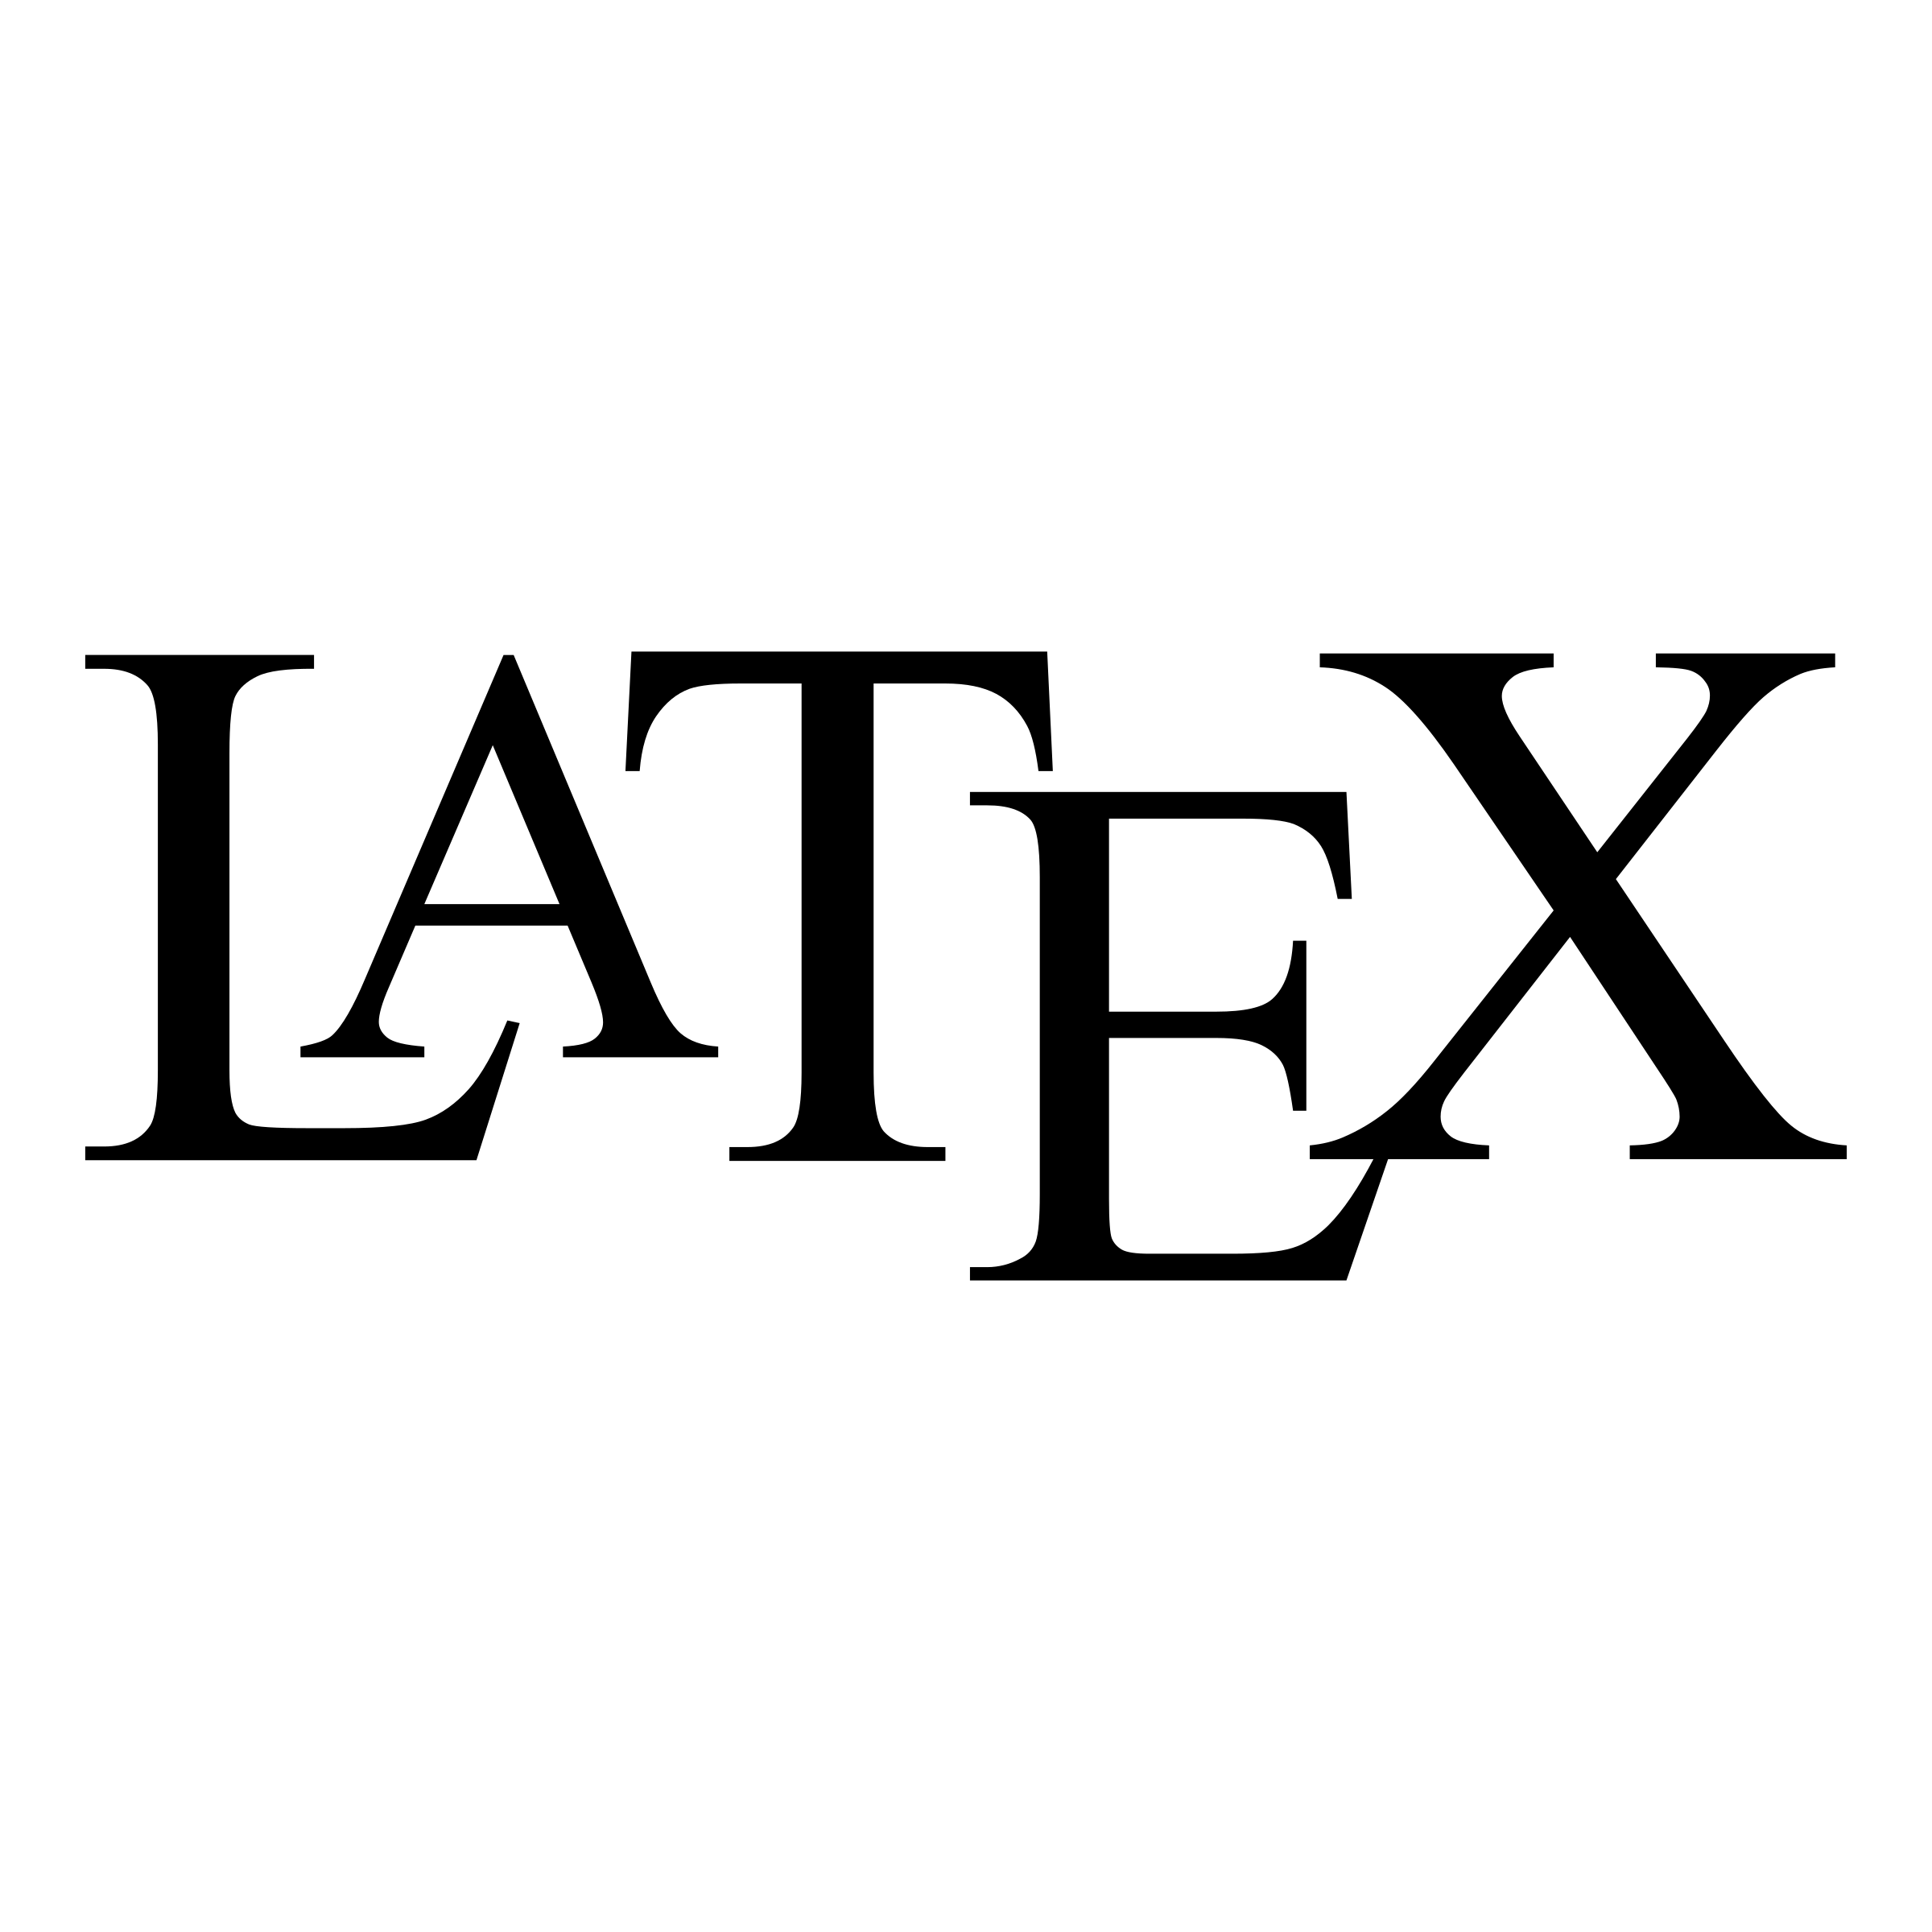
\includegraphics[draft, scale=0.02]{LatexLogo.png}

\subsection{Float Figure}
\subsubsection{Overview}
\begin{figure}[!htbp]
    \centering
    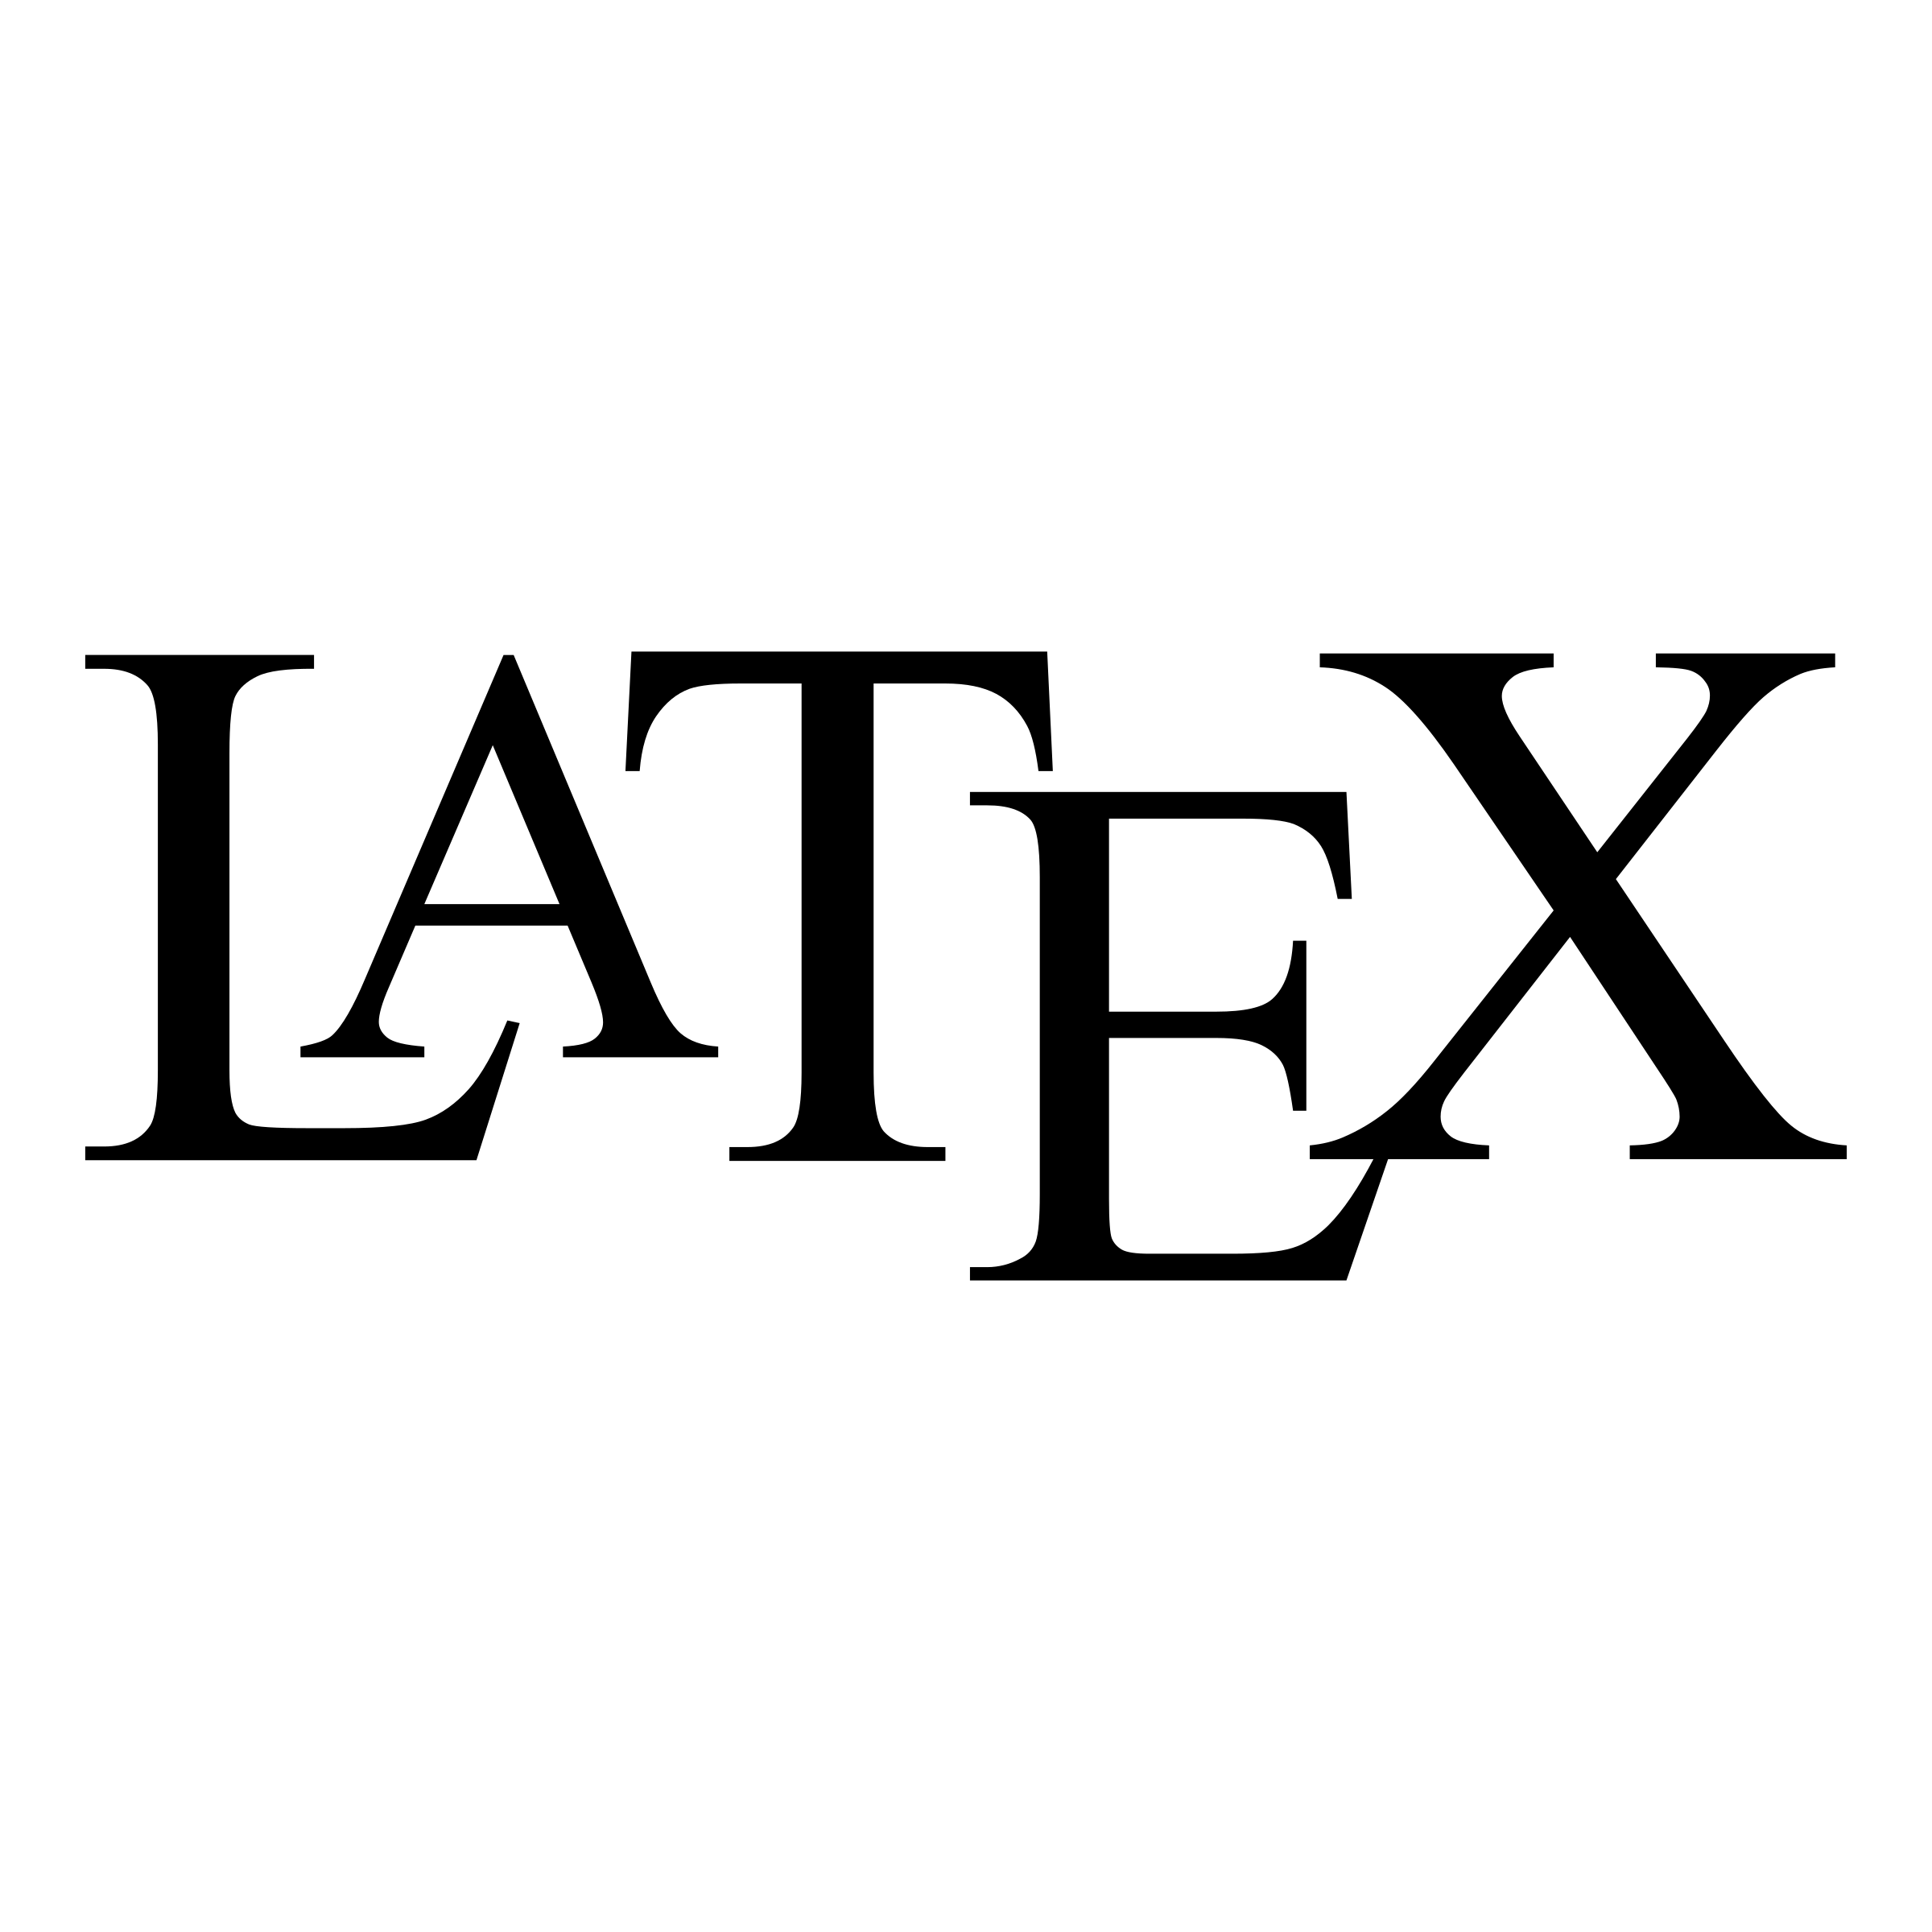
\includegraphics[scale=0.05]{LatexLogo.png}
    \bicaption[Latex Logo]{\label{fig-float} Latex Logo - Example Of Float Figure}[标志]{浮动图片的例子}
\end{figure}

\subsubsection{Rotated Figure}
% must usepackage rotfloat
\begin{sidewaysfigure}
    \centering
    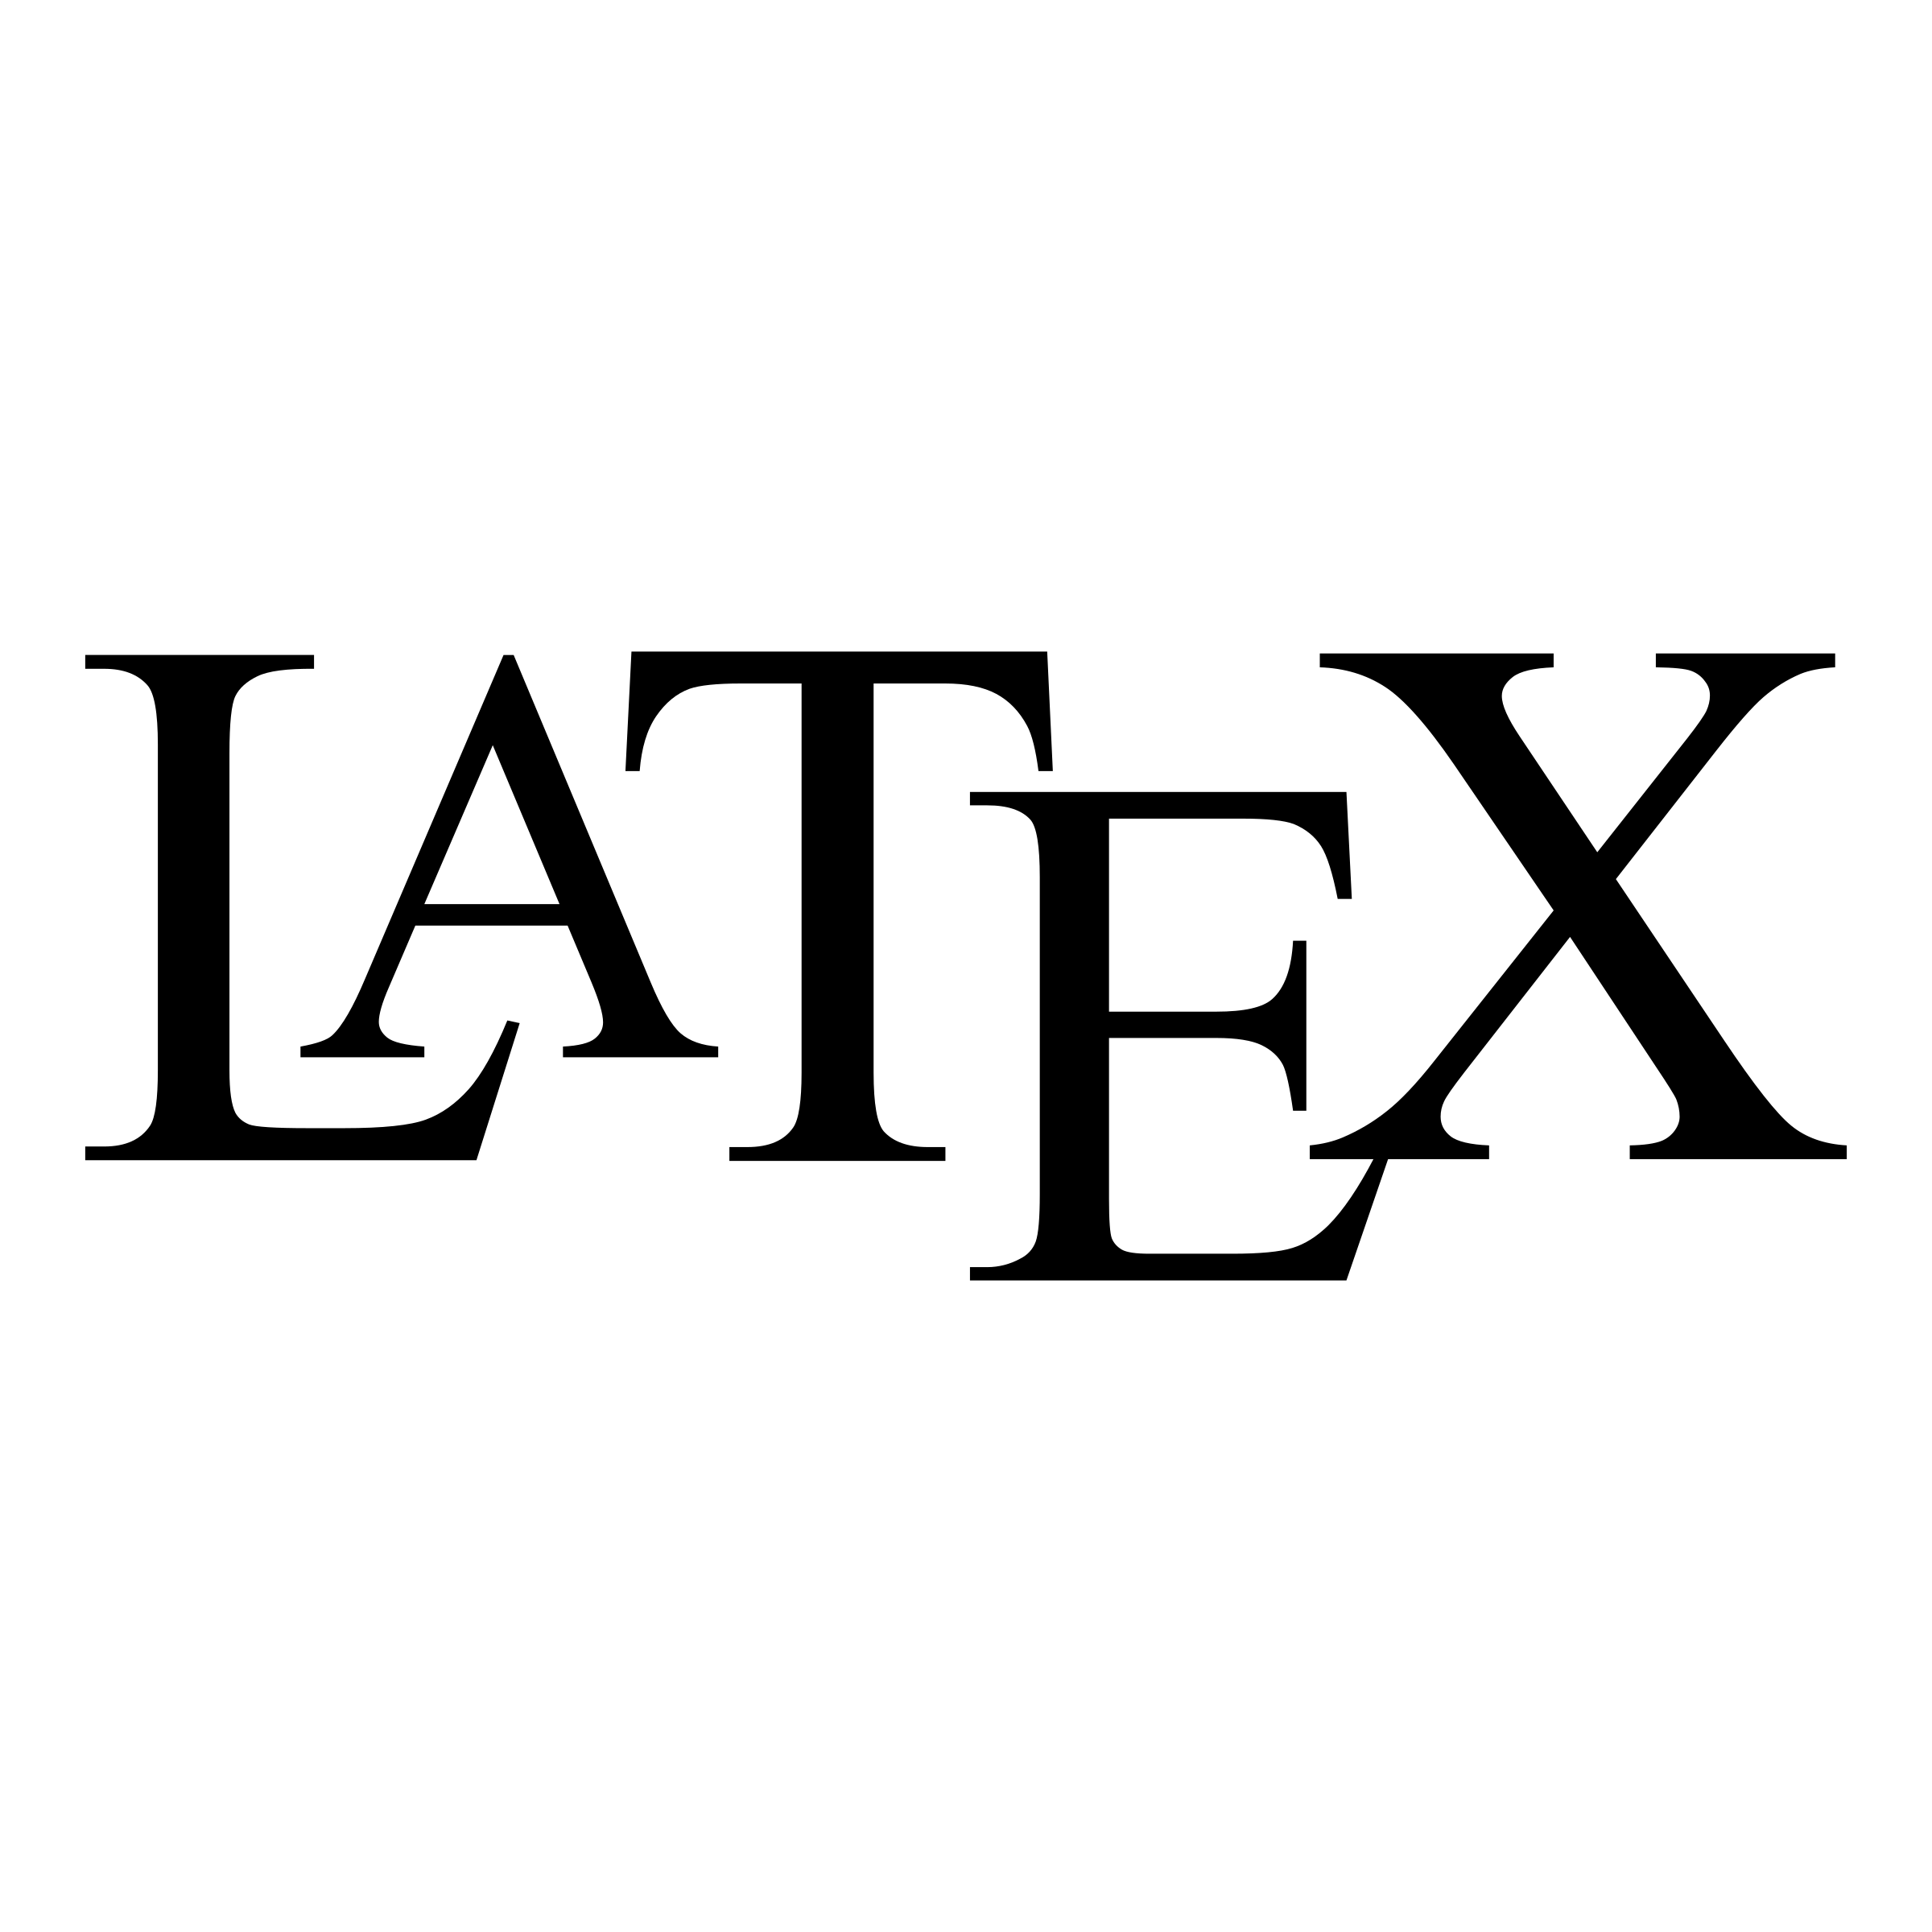
\includegraphics[scale=0.1]{LatexLogo.png}
    \caption{Latex Logo}
\end{sidewaysfigure}

\subsubsection{Side By Side}
\paragraph{Figure With Words}
\begin{figure}[H]
    \centering
    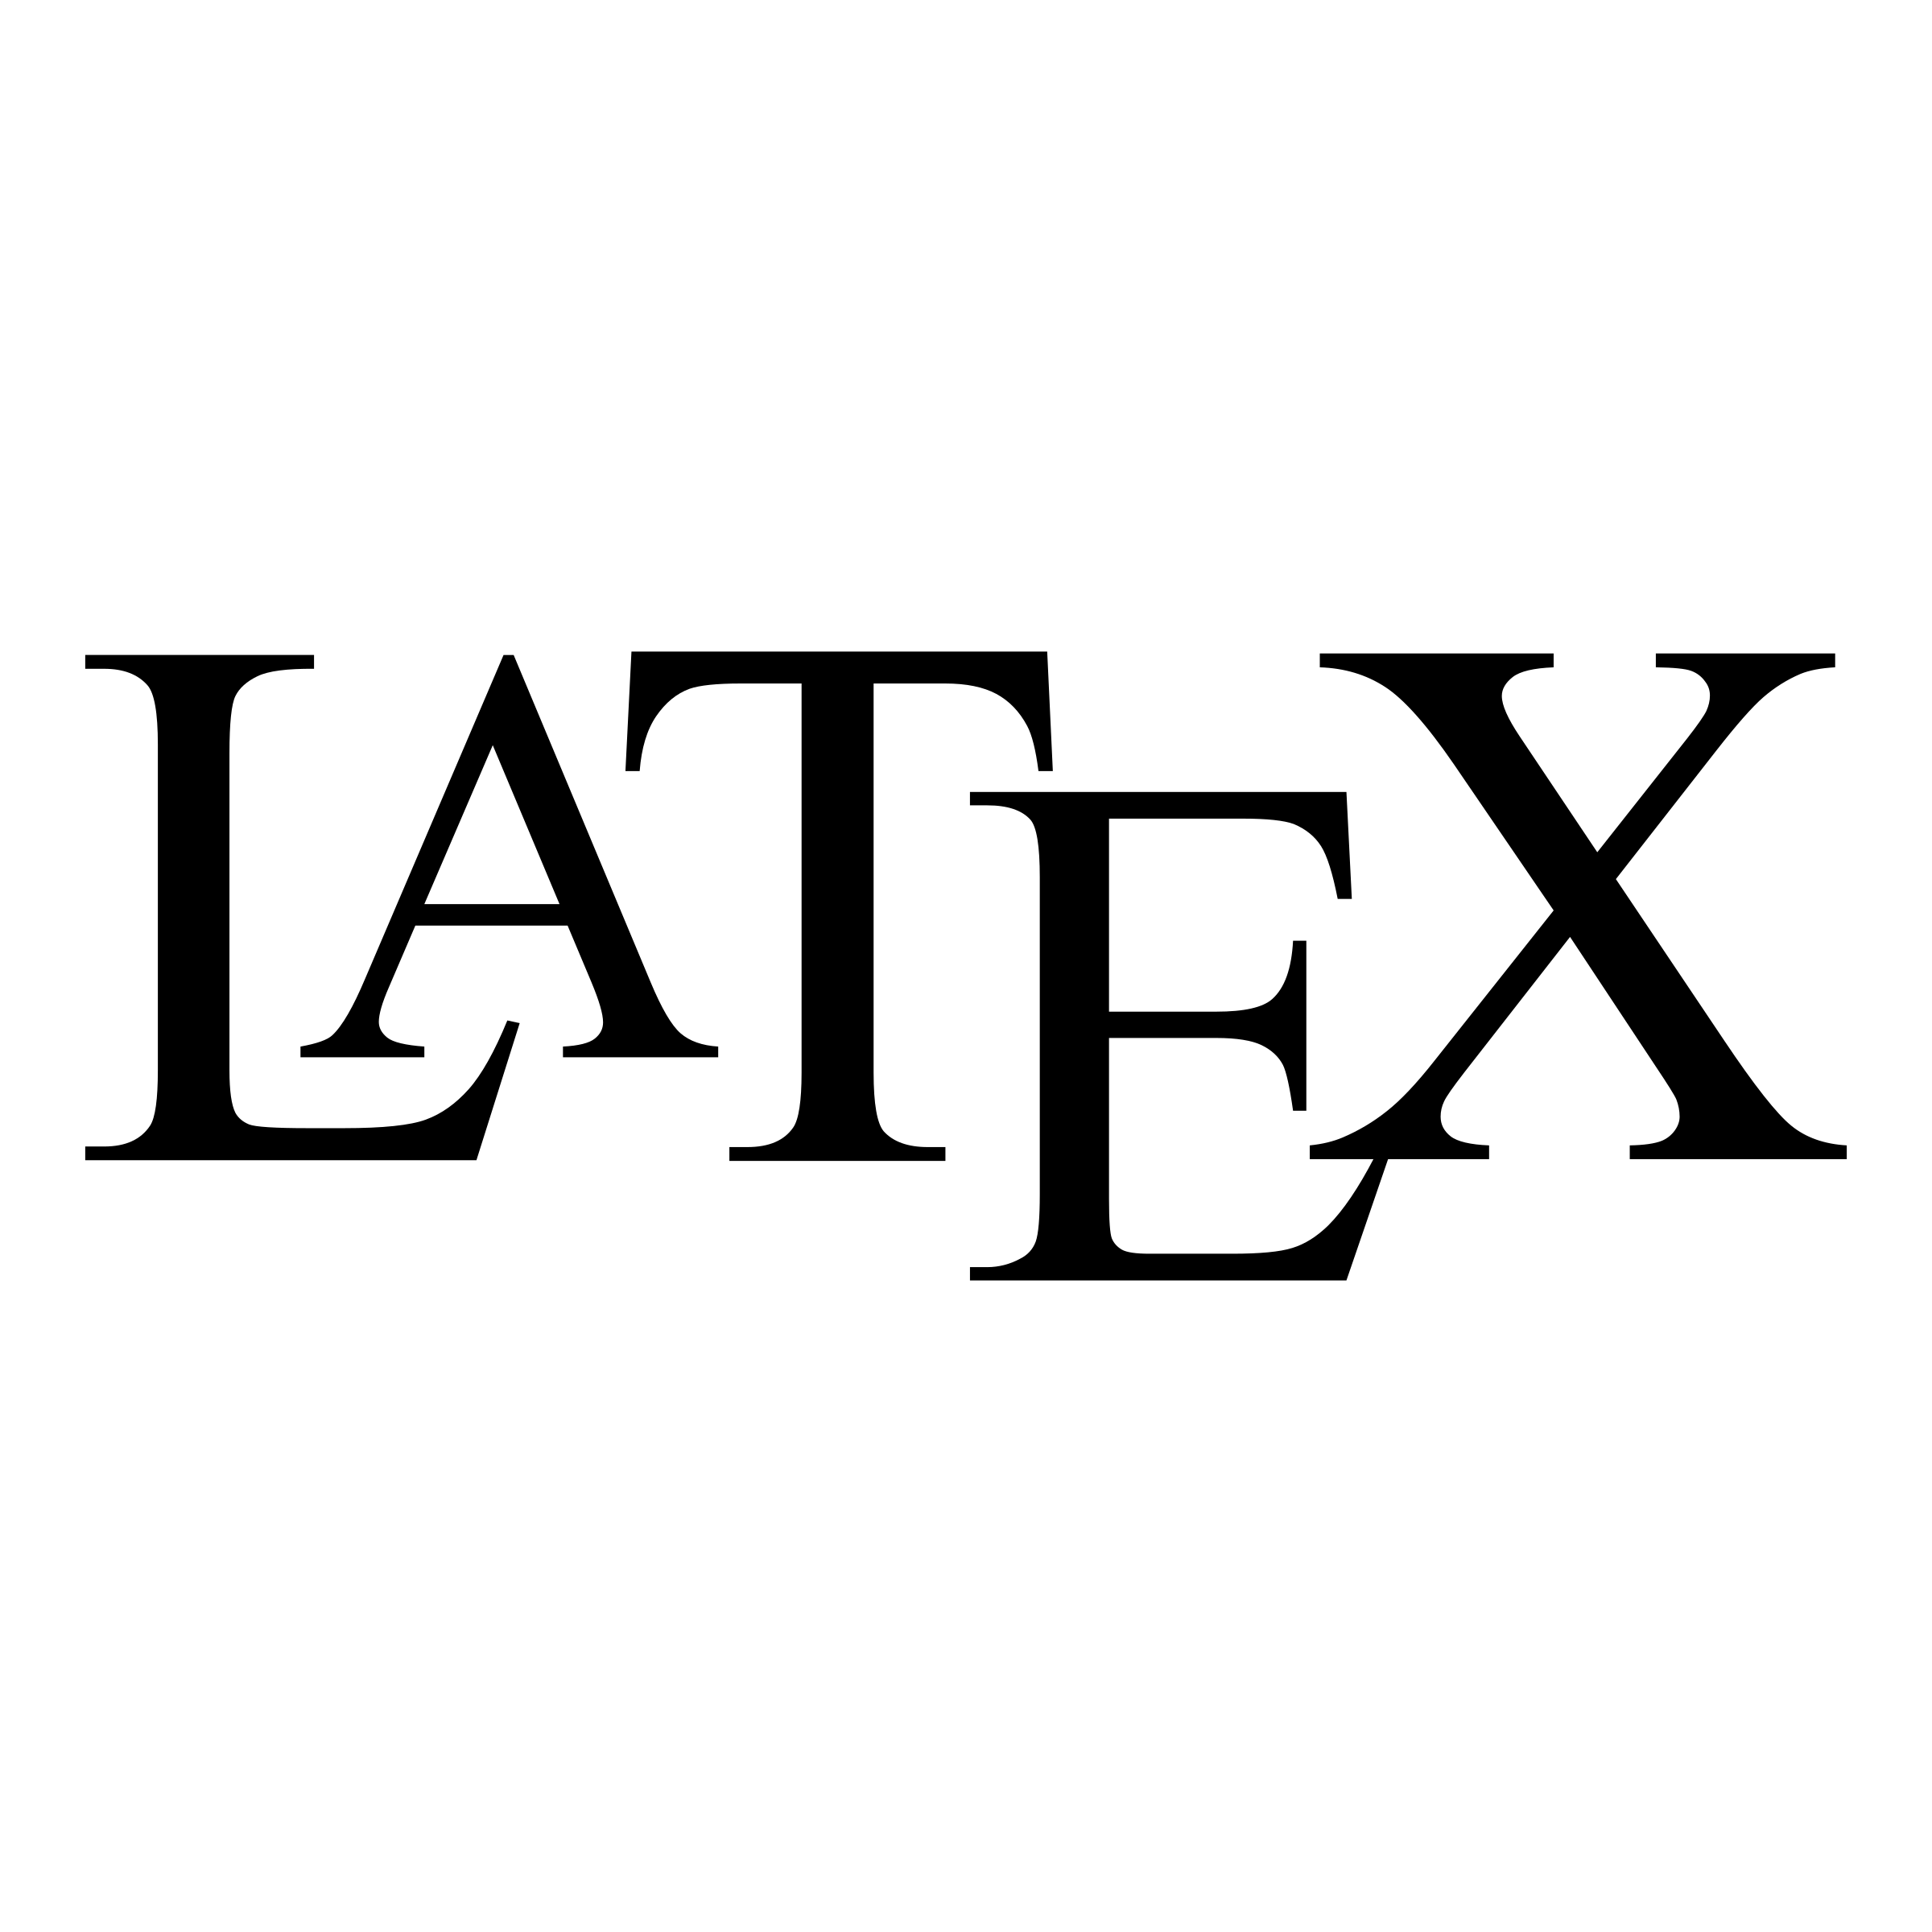
\includegraphics[width=0.4\textwidth]{LatexLogo.png}
    \qquad
    \parbox[b]{0.4\textwidth}{This is the comment on the figure.}
    \caption{Figure With Words Example}
\end{figure}

\paragraph{Figures Side By Side}
\begin{figure}[H]
    \centering
    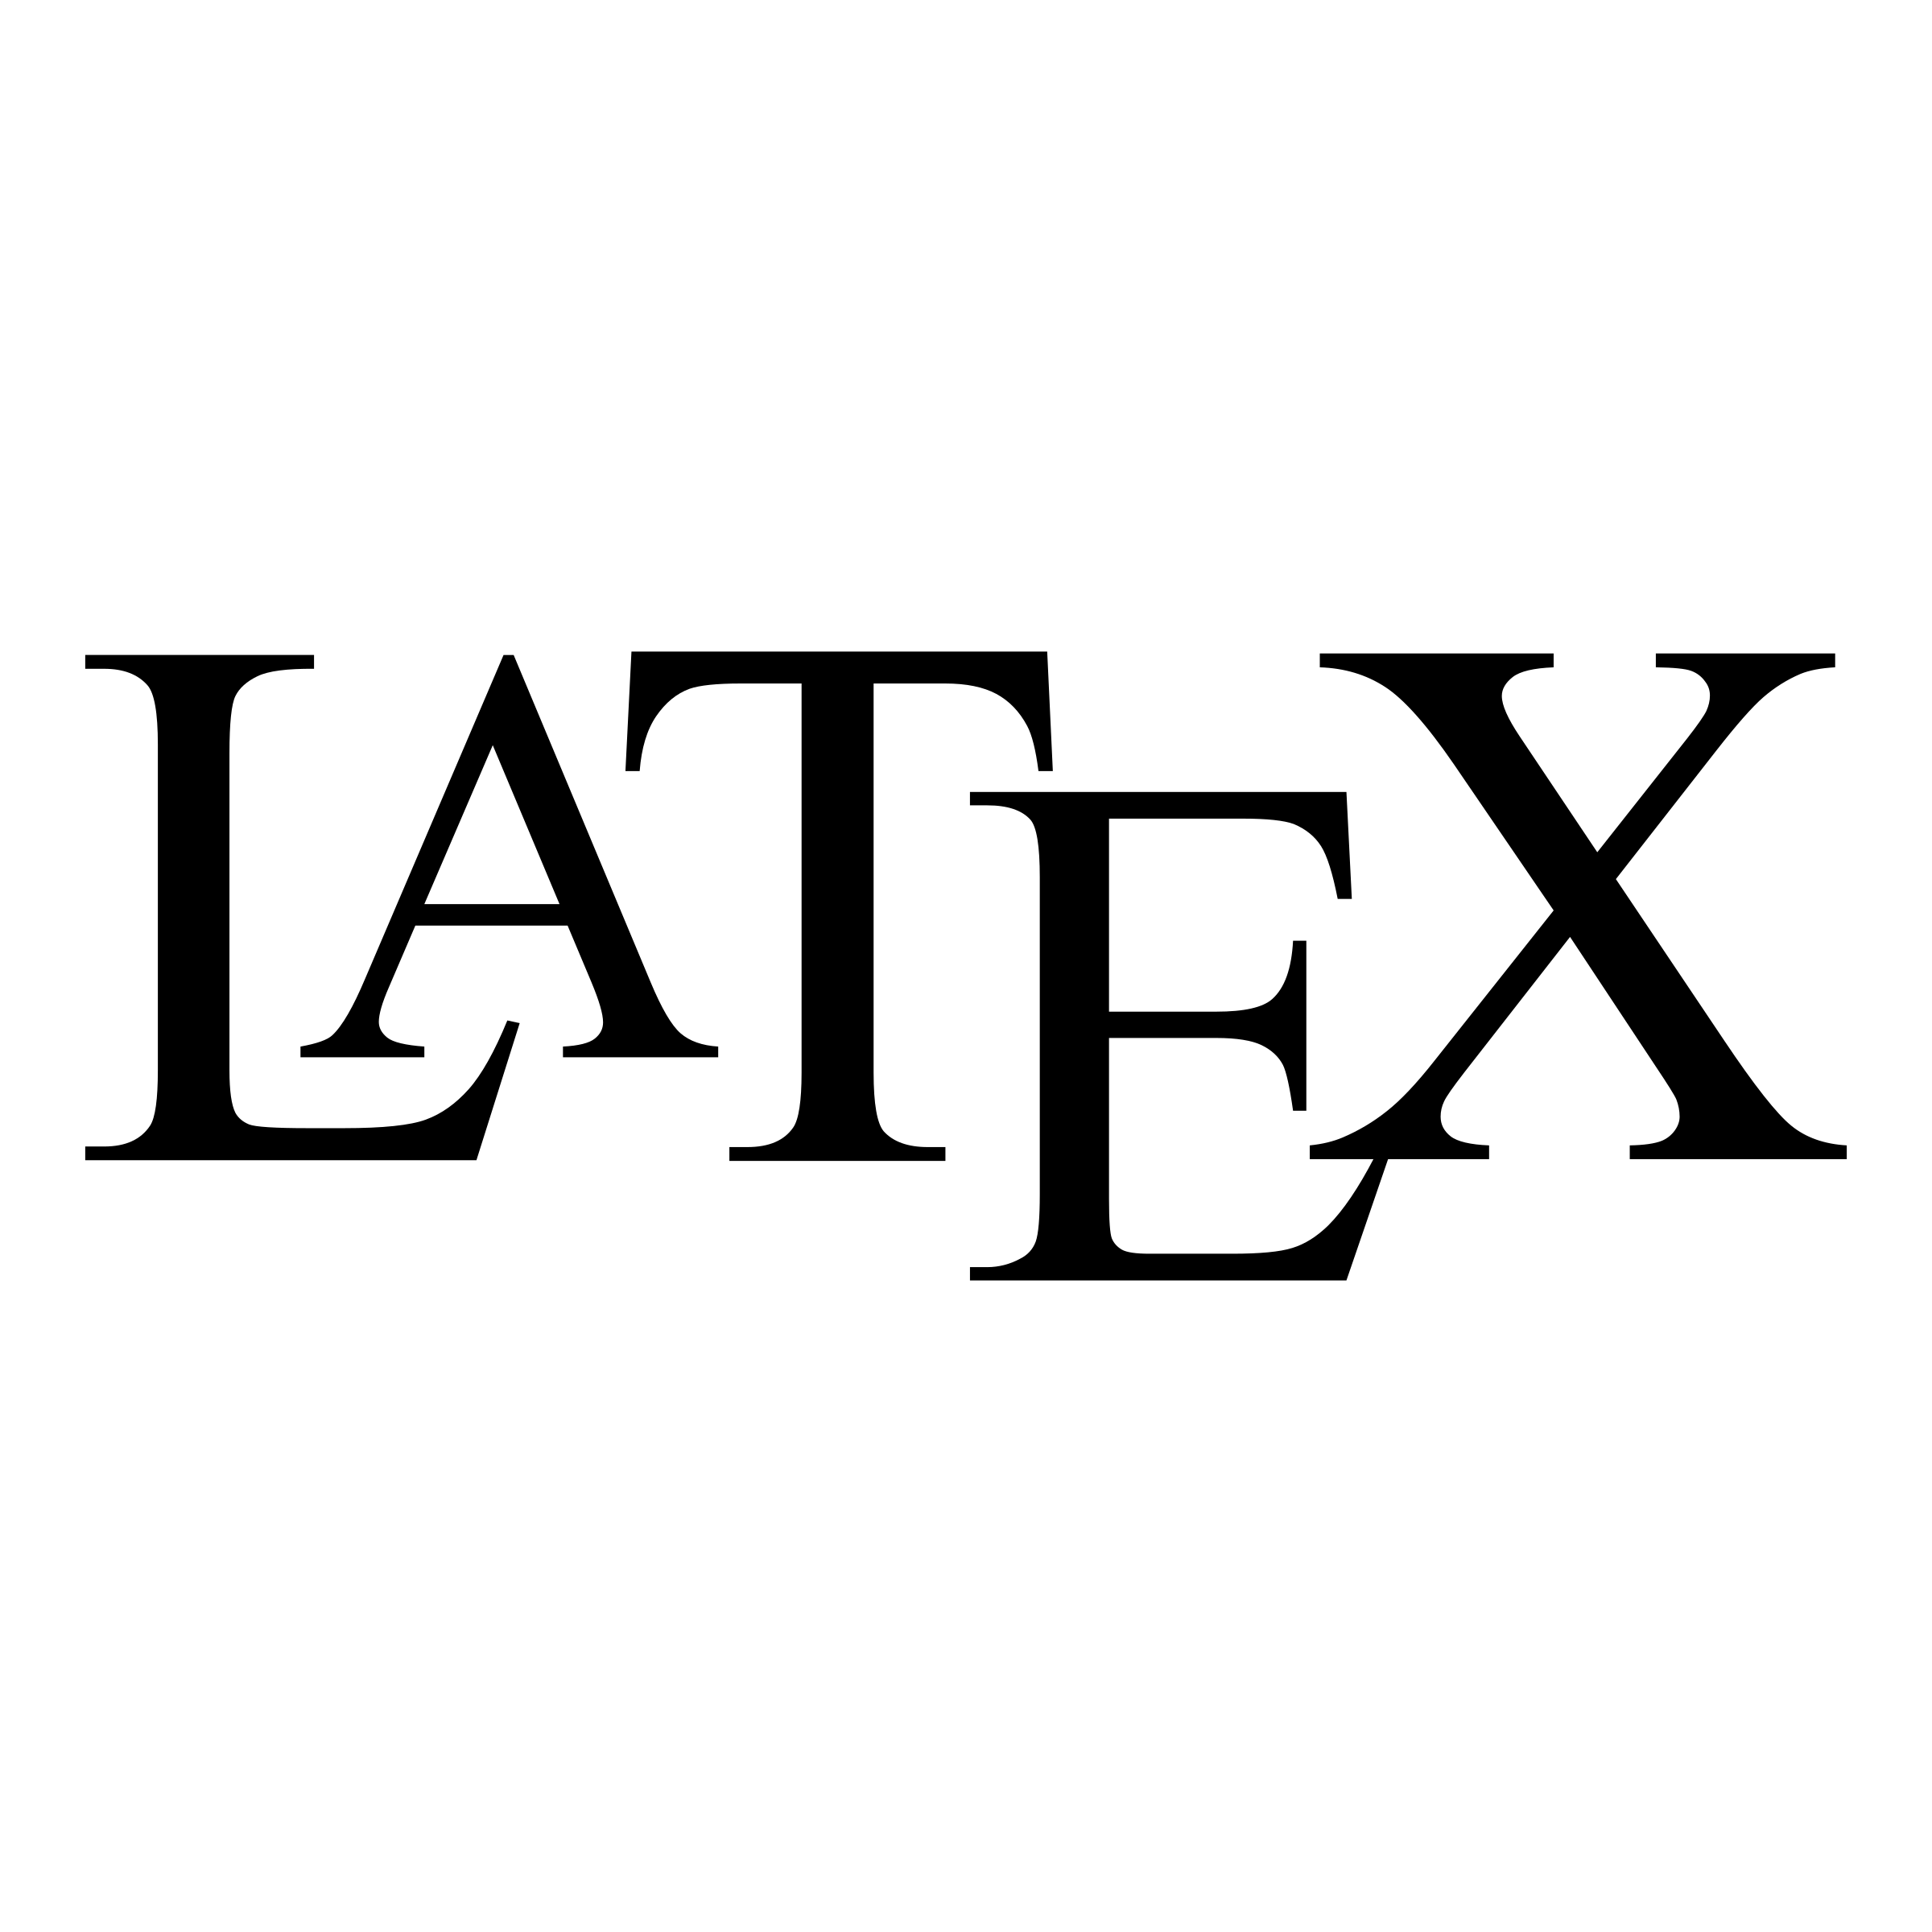
\includegraphics[width=0.4\textwidth]{LatexLogo.png}
    \qquad
    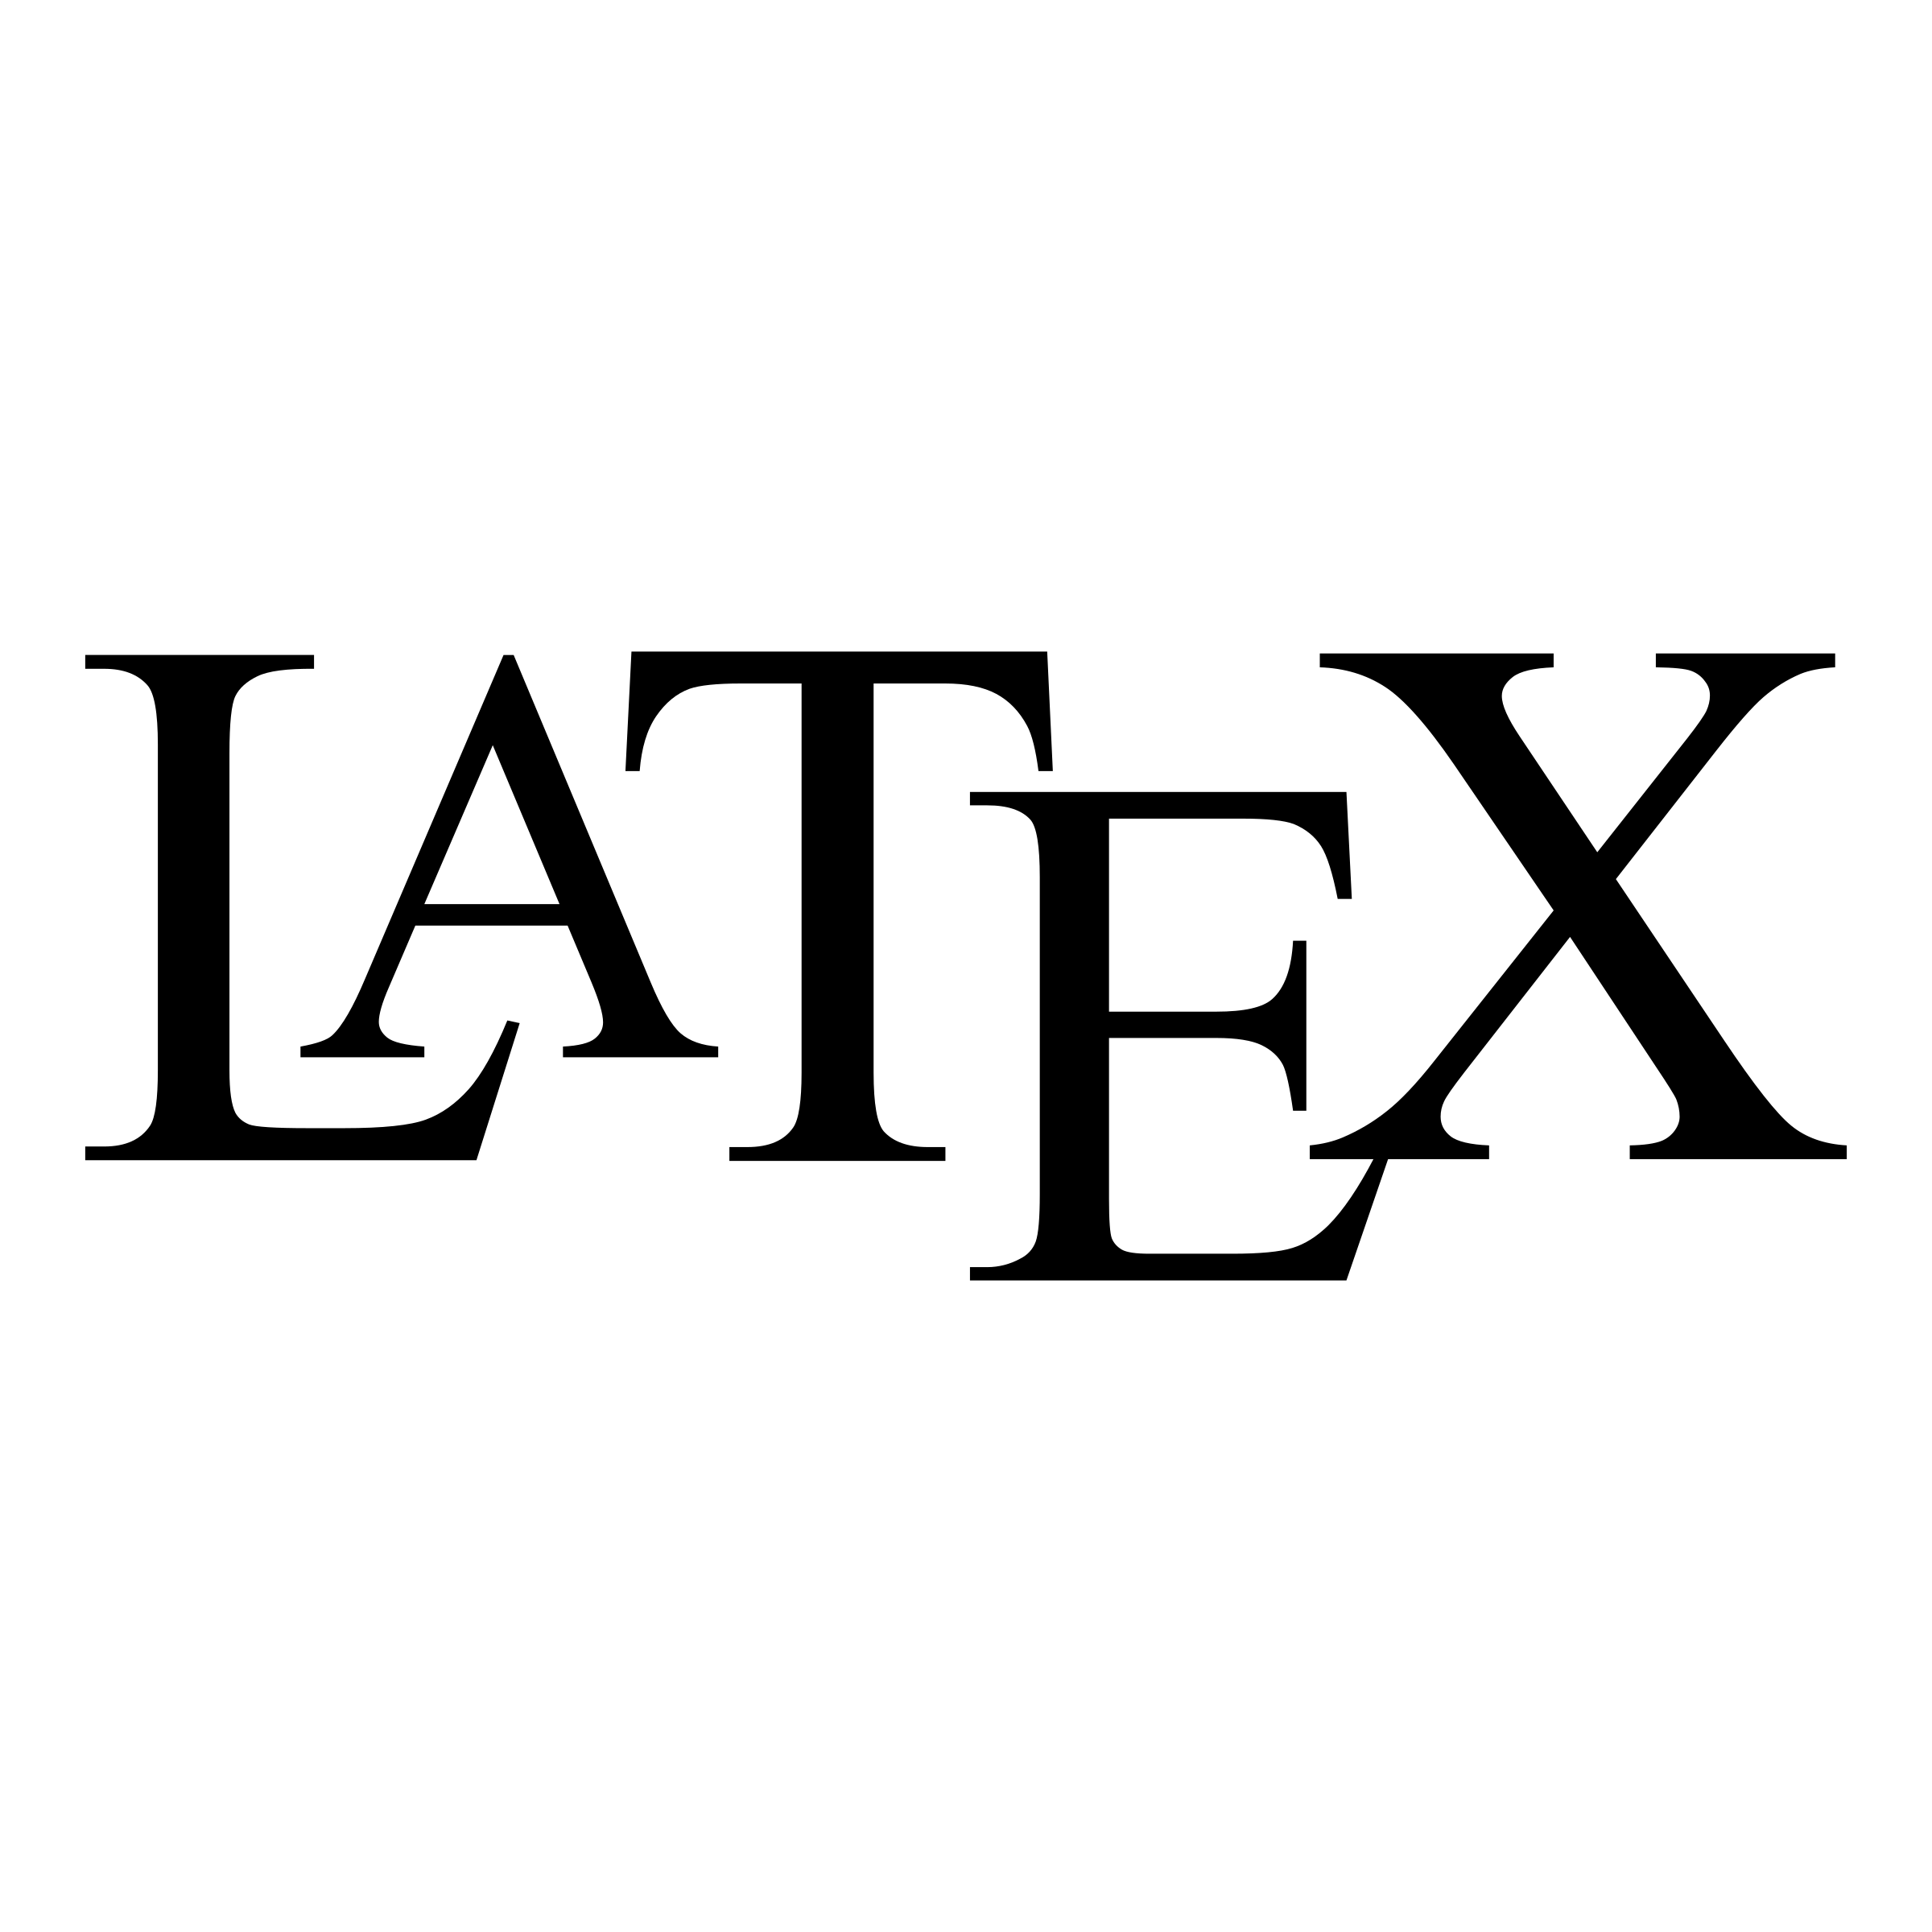
\includegraphics[width=0.4\textwidth]{LatexLogo.png}
    \caption{Figure Side By Side Example}
\end{figure}

\paragraph{Captions For Side By Side}
\begin{figure}[H]
    \caption{Title For Both}
    \parbox[b]{0.5\textwidth}{\centering
        \caption{Title For Left}
        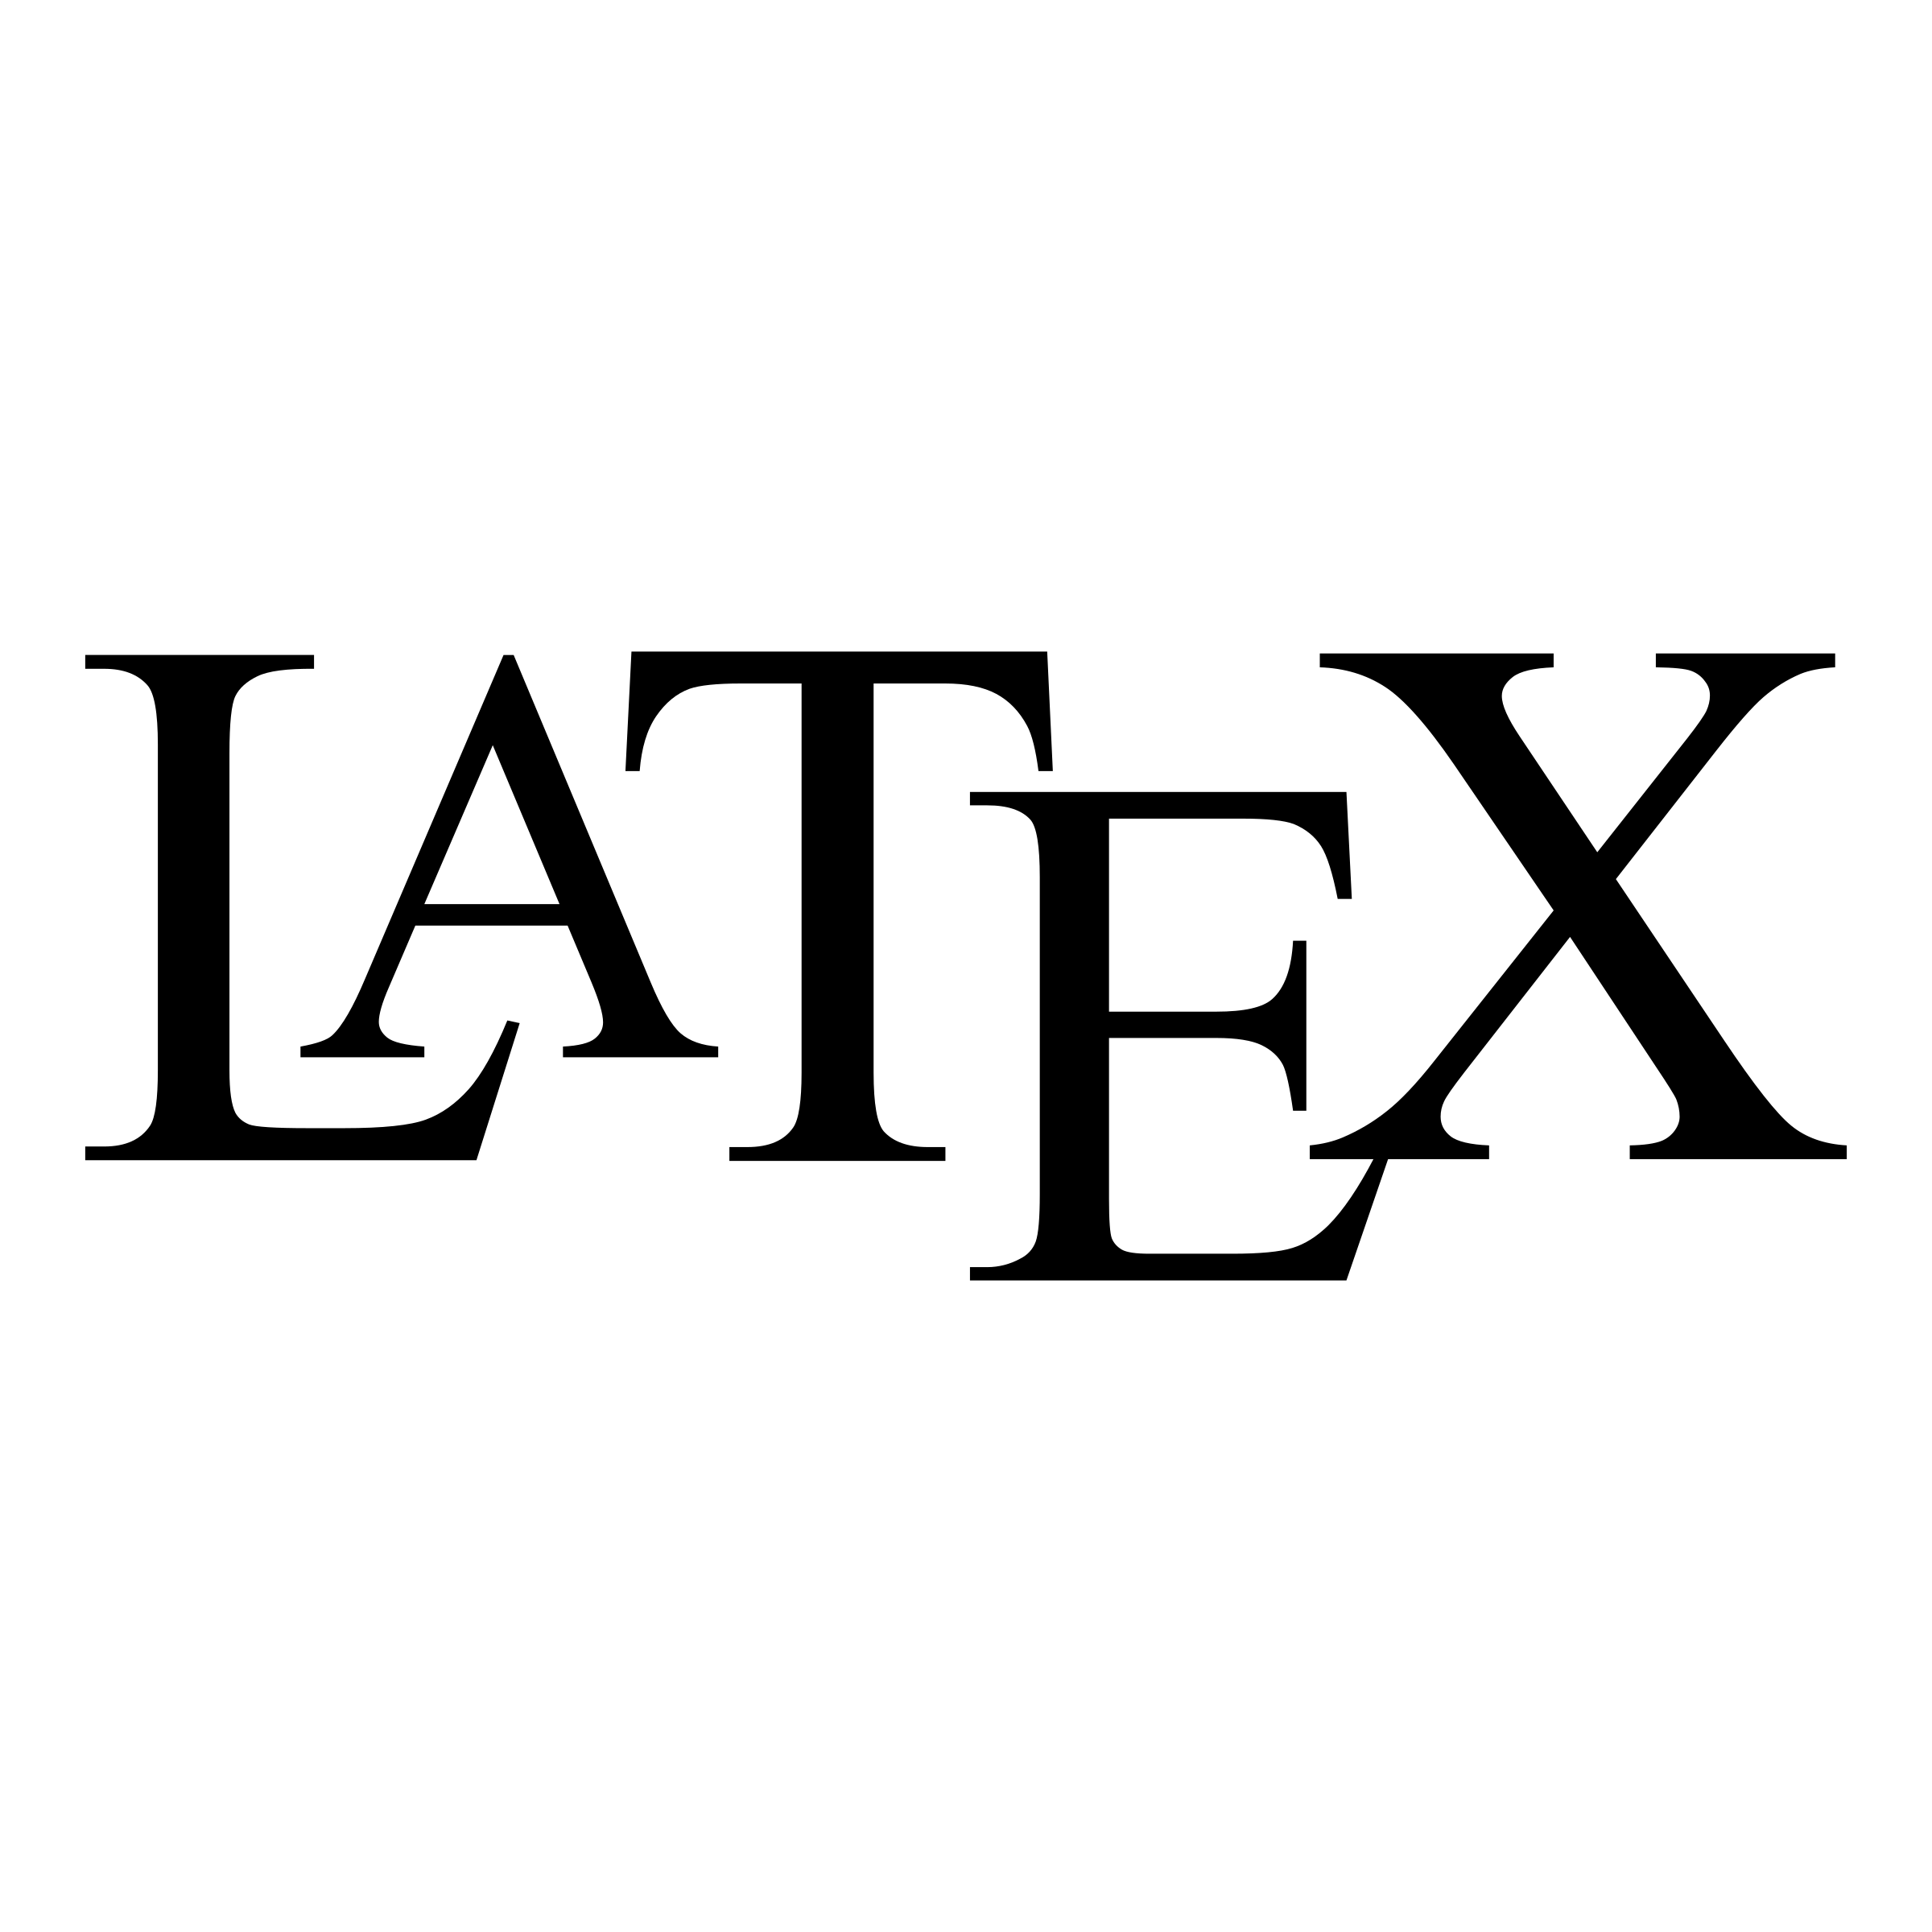
\includegraphics[width=0.4\textwidth]{LatexLogo.png}}
    \parbox[b]{0.5\textwidth}{\centering
        \caption{Title For Right}
        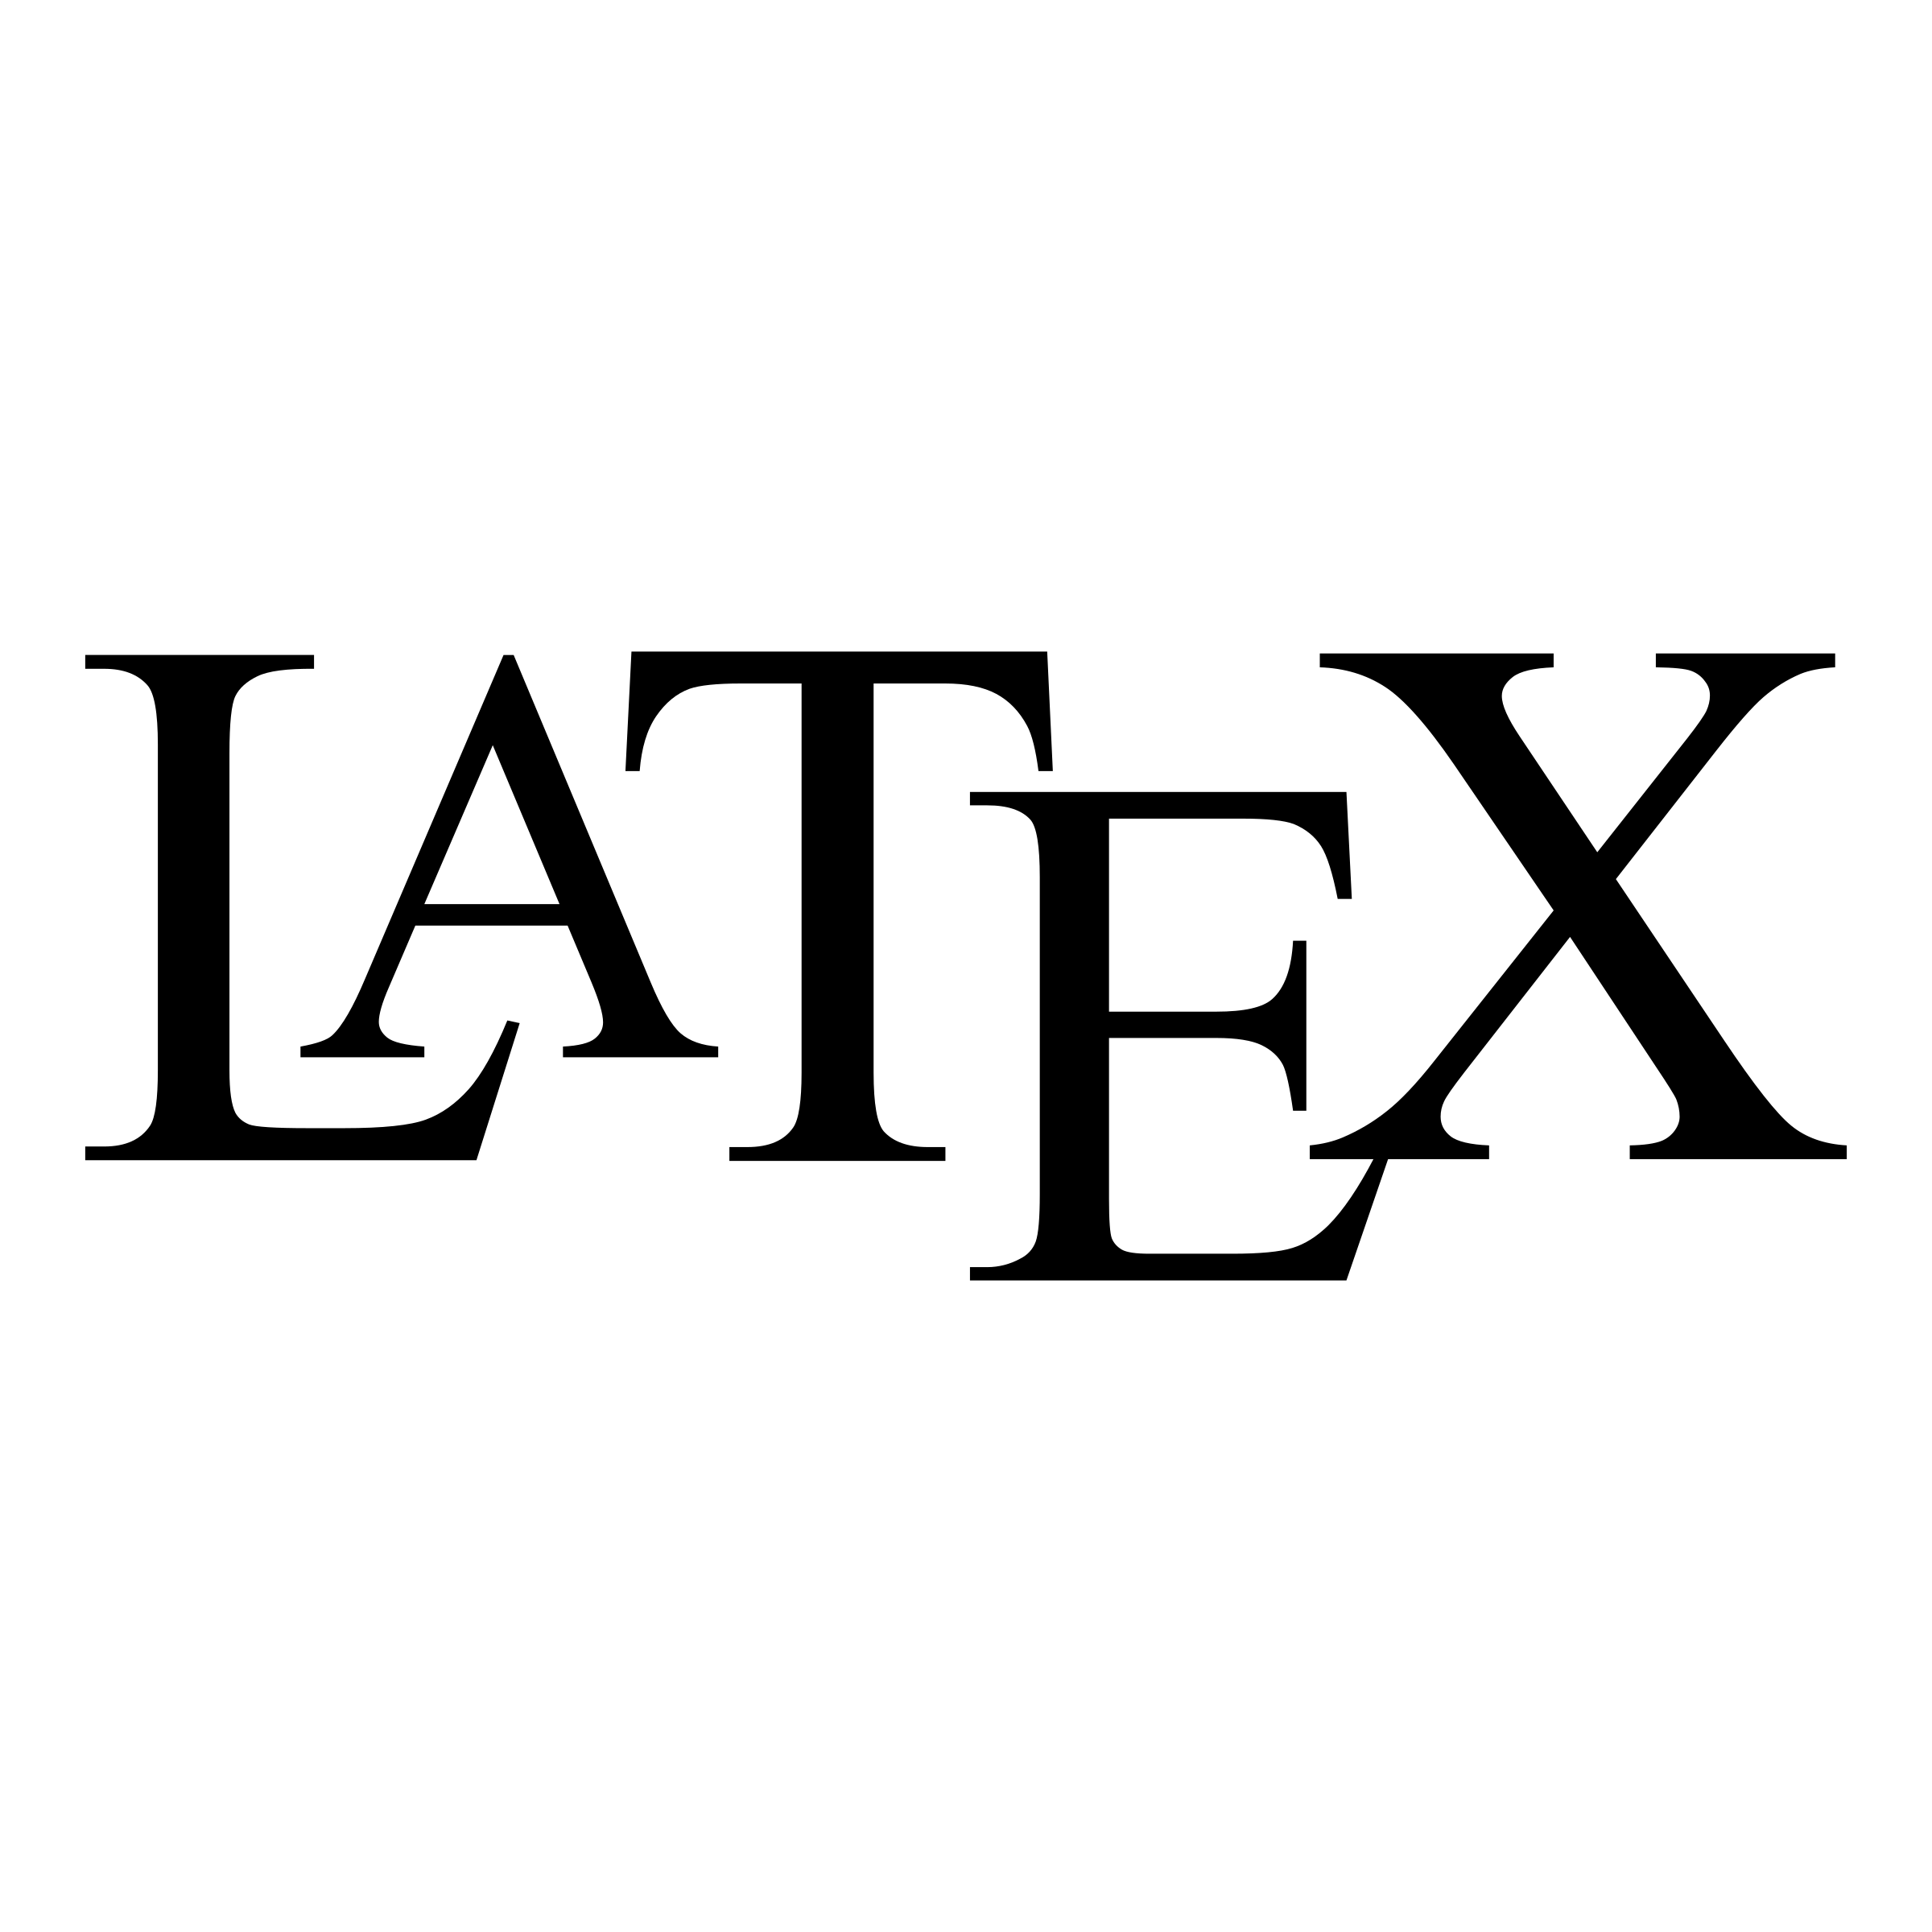
\includegraphics[width=0.4\textwidth]{LatexLogo.png}}
\end{figure}

\begin{figure}[H]
    % must usepackage subcaption
    \caption{Title For Both}
    \begin{subfigure}[b]{0.5\textwidth}
        \centering
        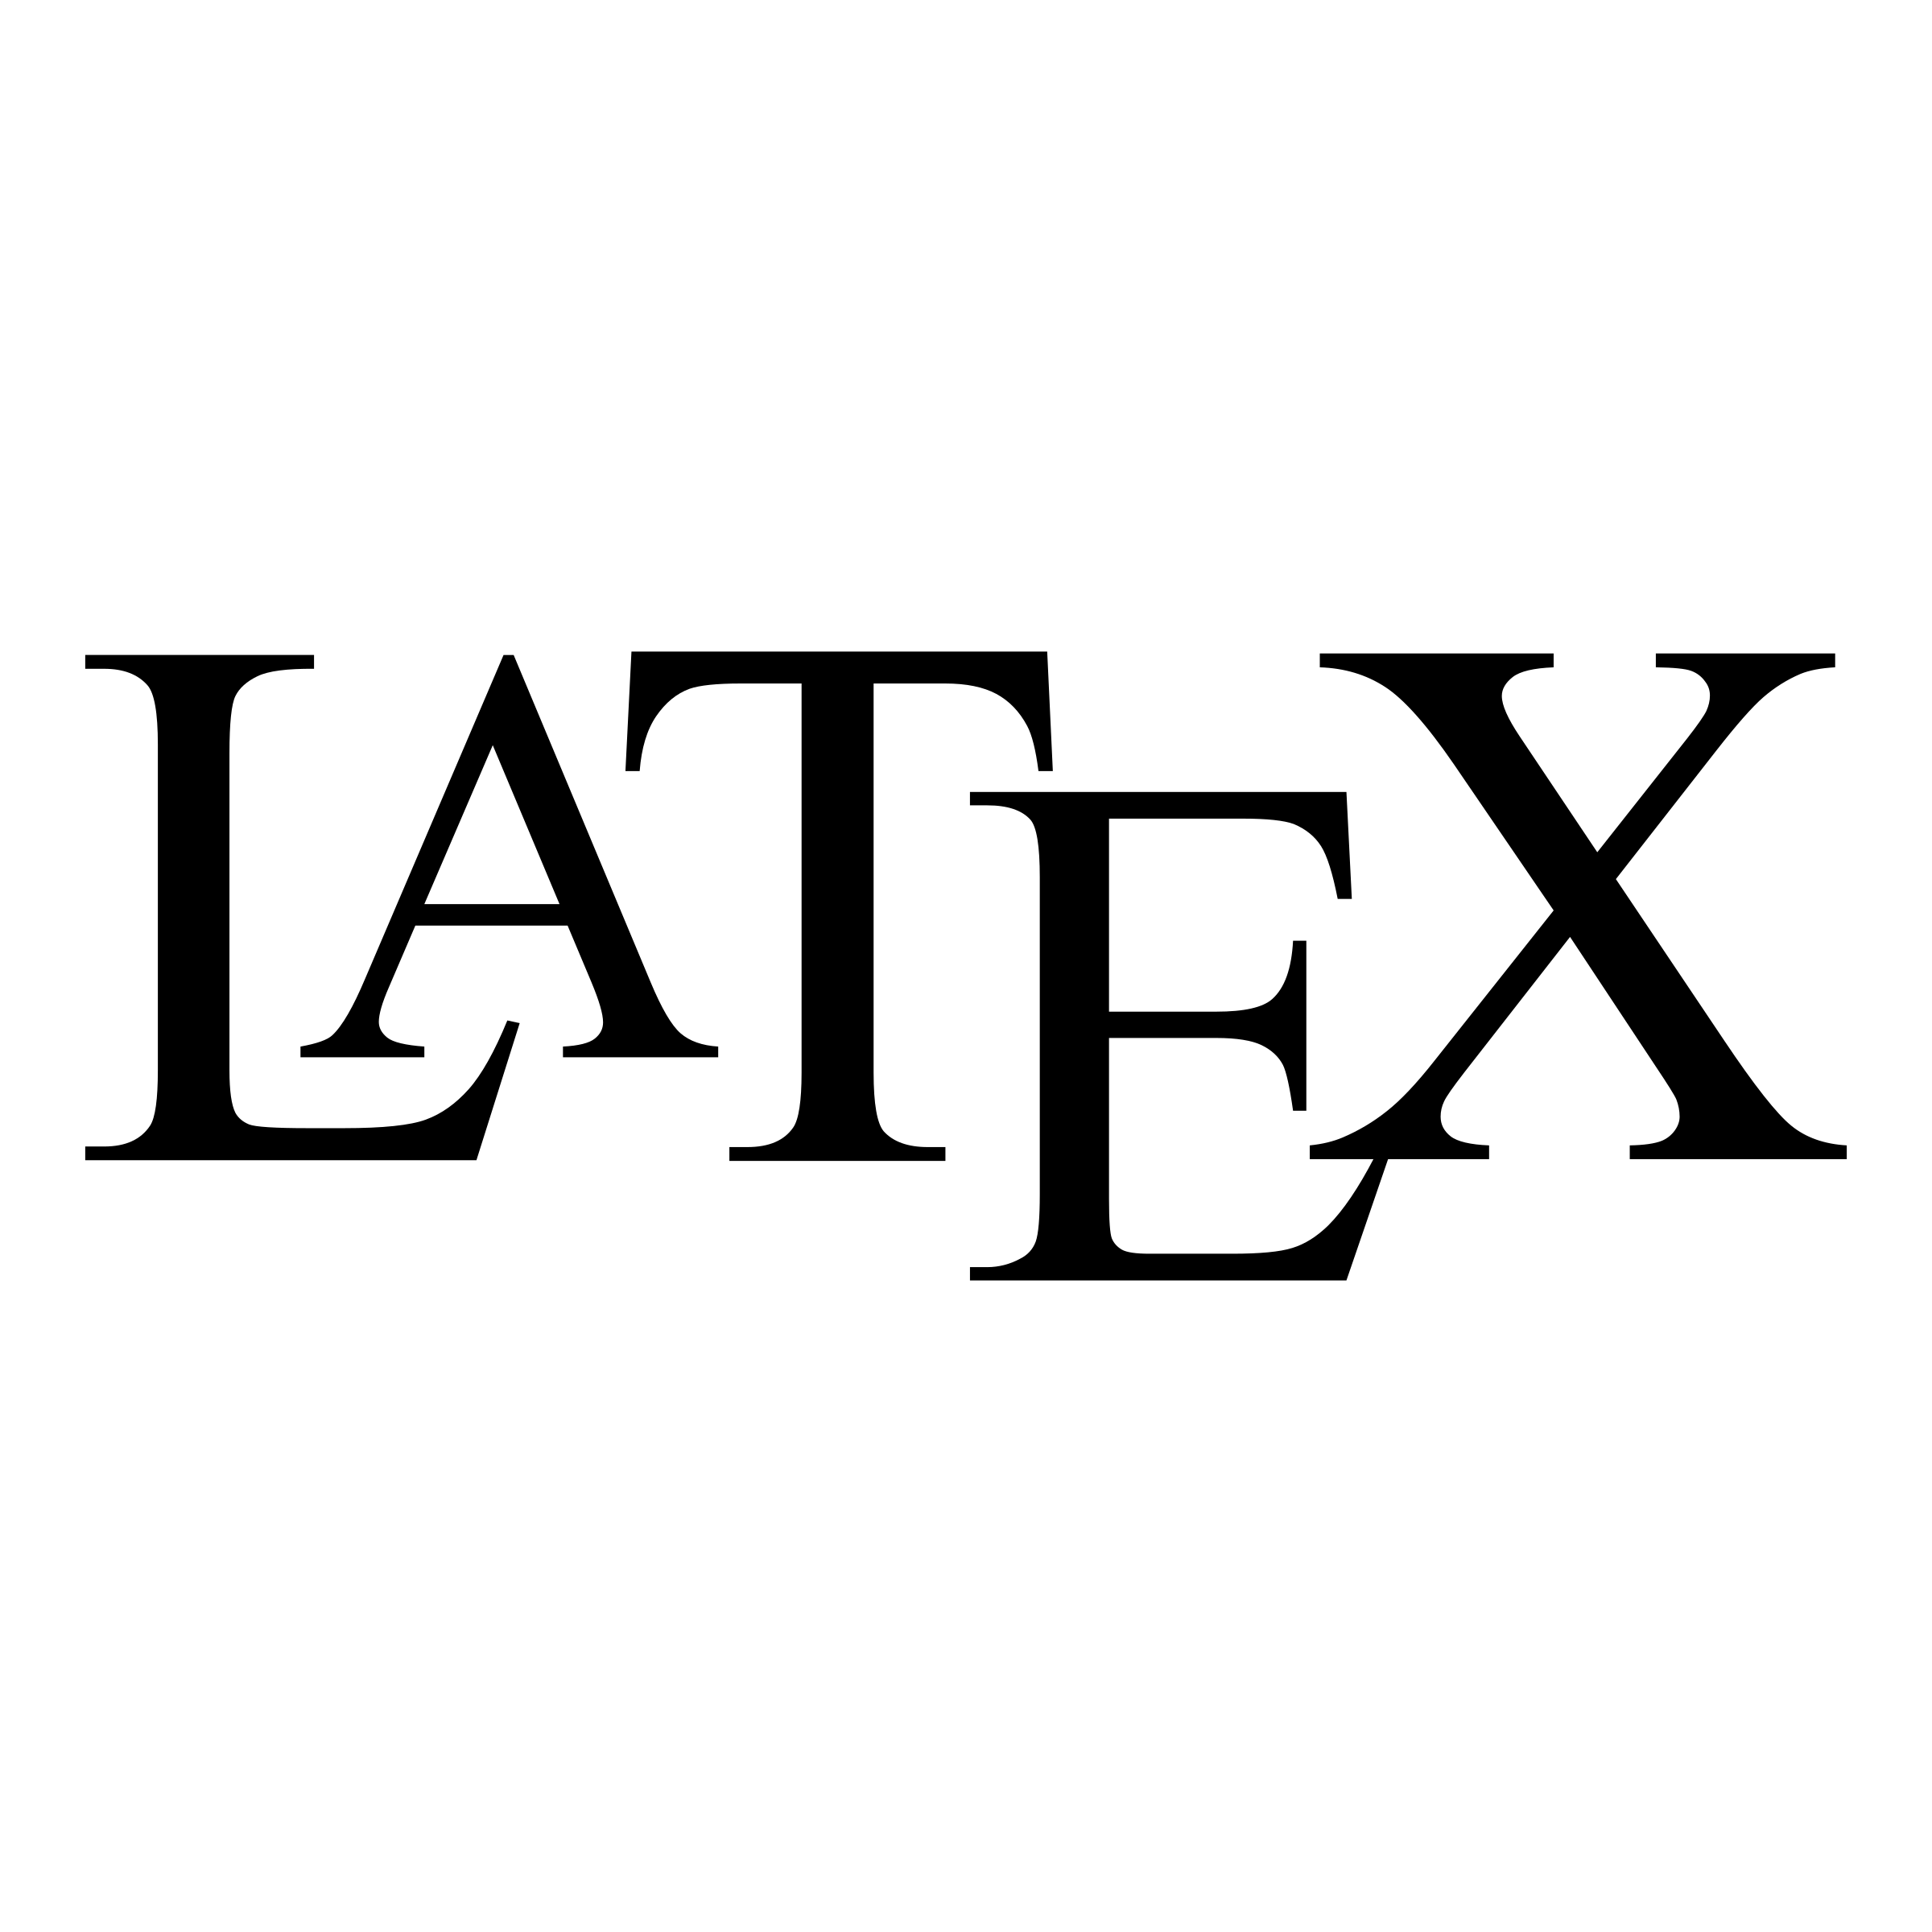
\includegraphics[width=0.4\textwidth]{LatexLogo.png}
        \caption{Title For Left}
    \end{subfigure}
    \begin{subfigure}[b]{0.5\textwidth}
        \centering
        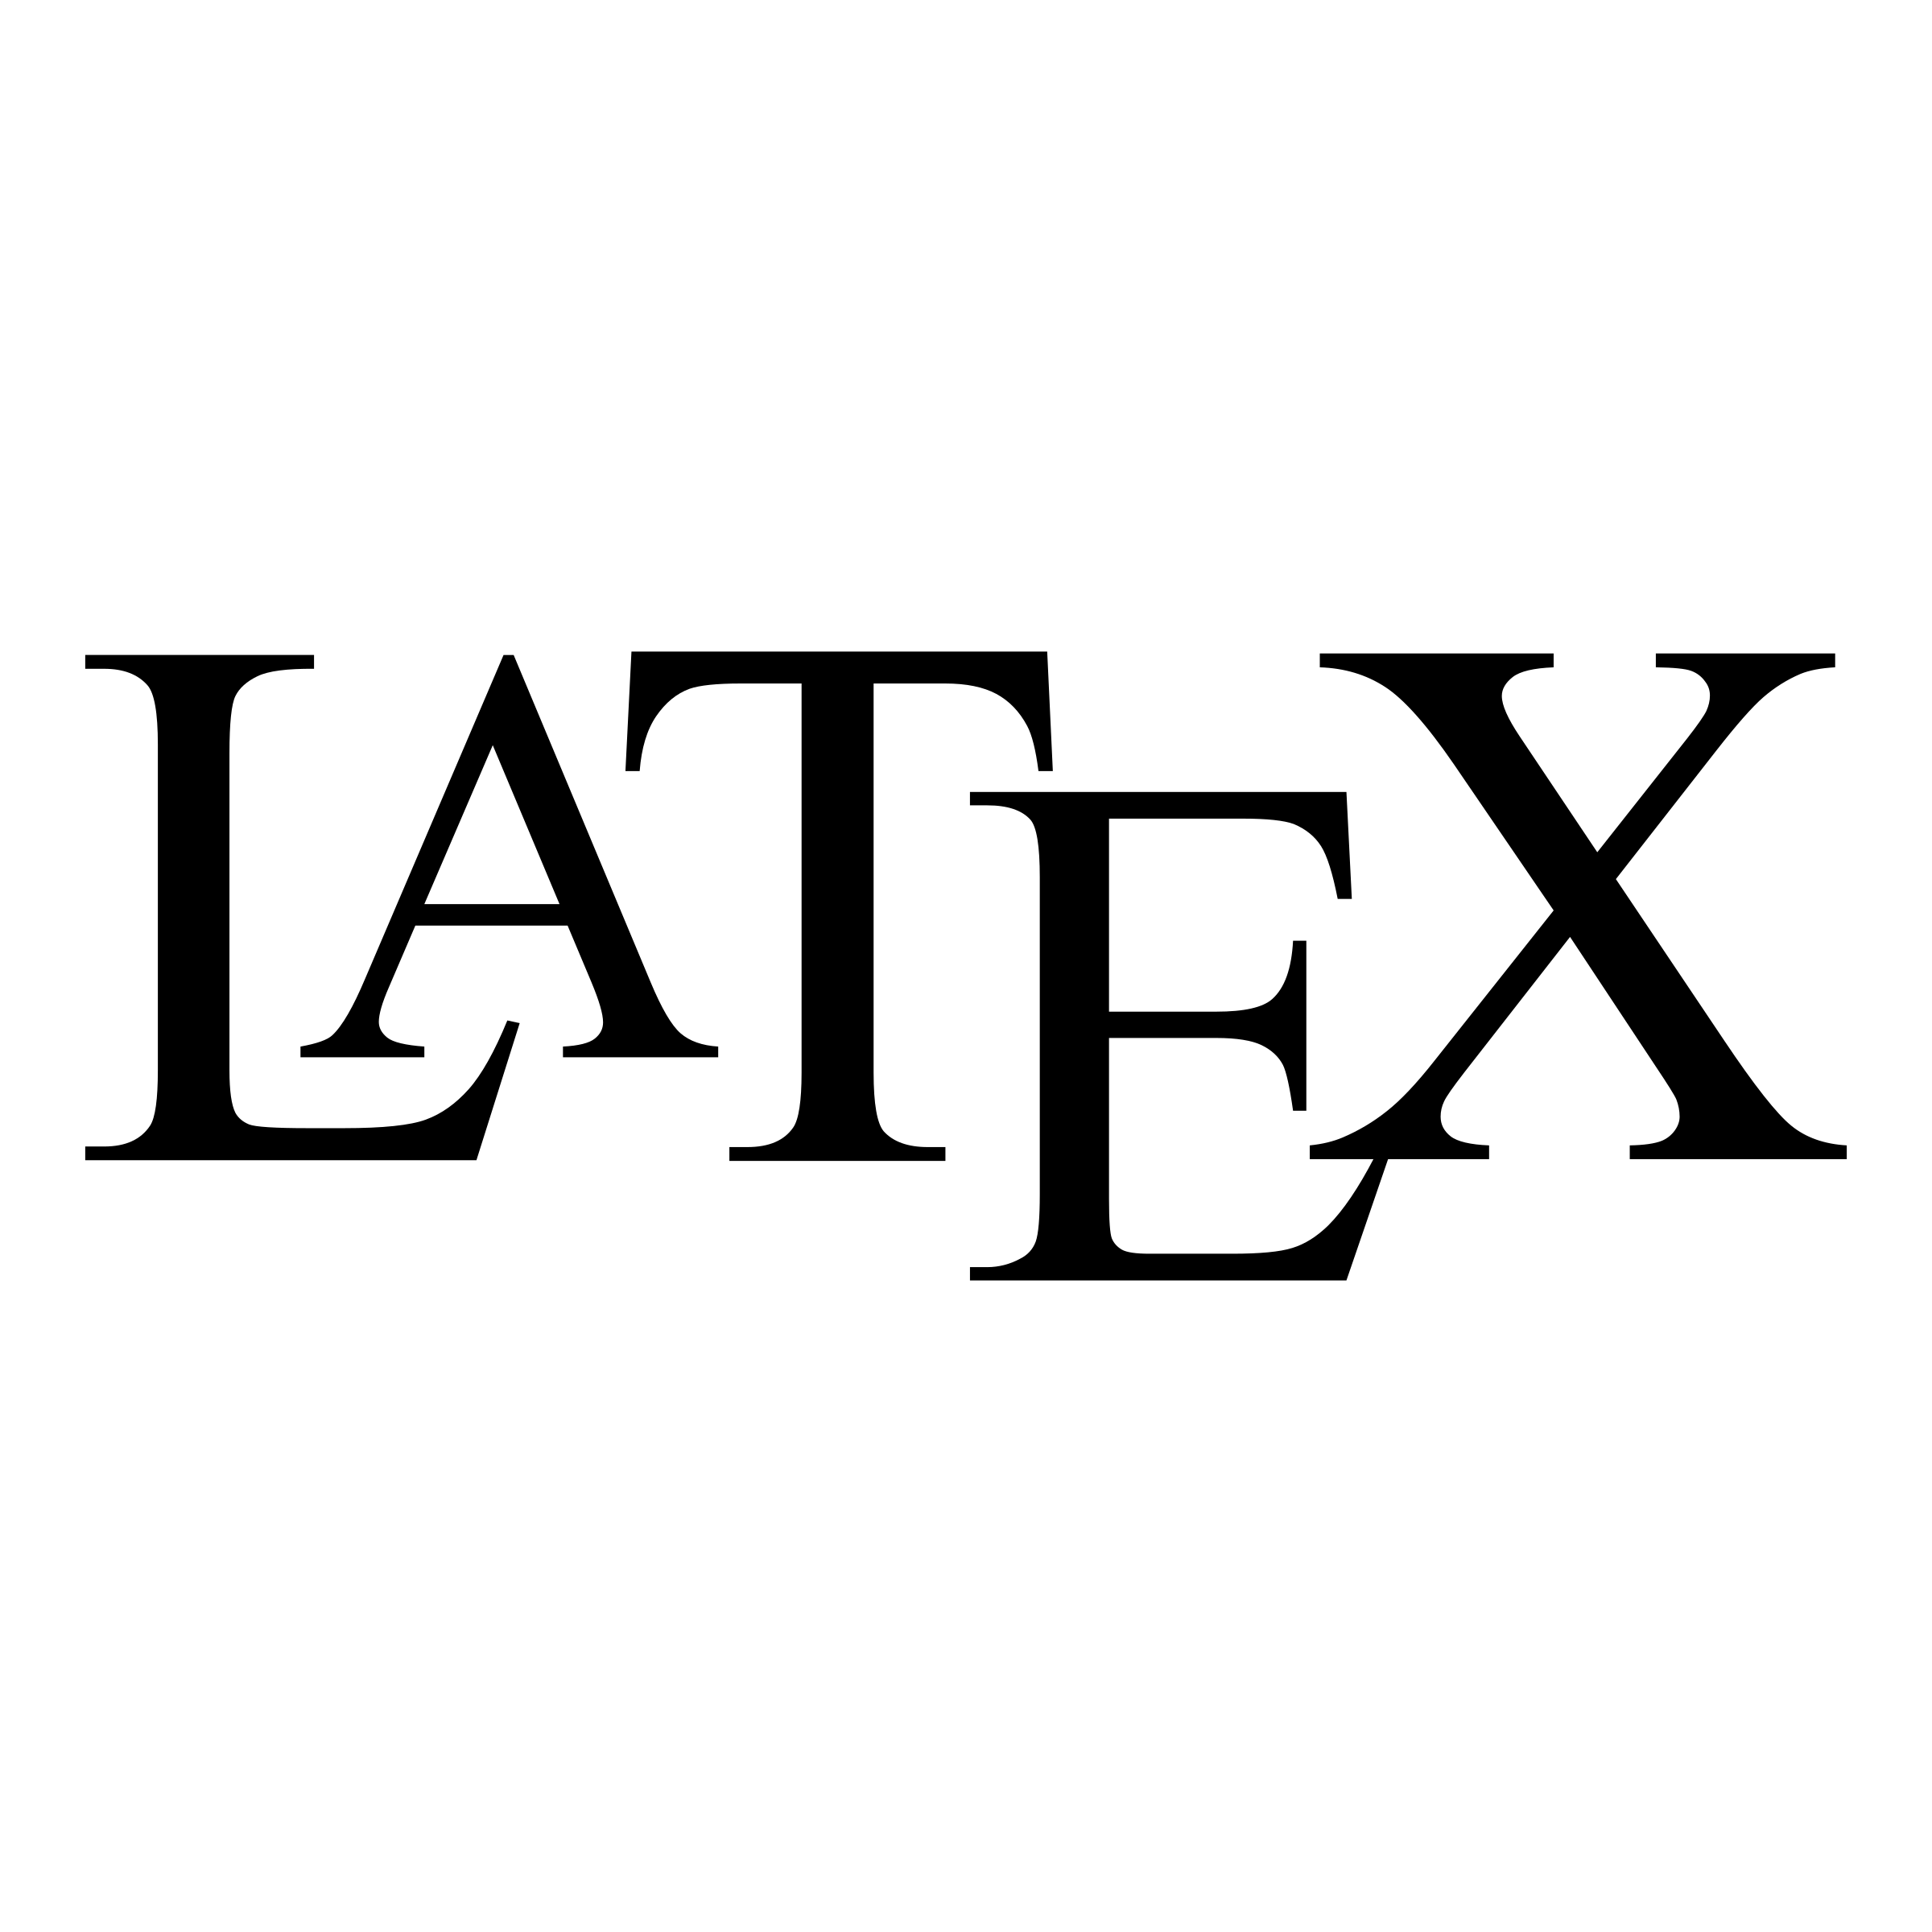
\includegraphics[width=0.4\textwidth]{LatexLogo.png}
        \caption{Title For Right}
    \end{subfigure}
\end{figure}

\subsubsection{Figure Arounded By Words}
\begin{figwindow}[2, r, 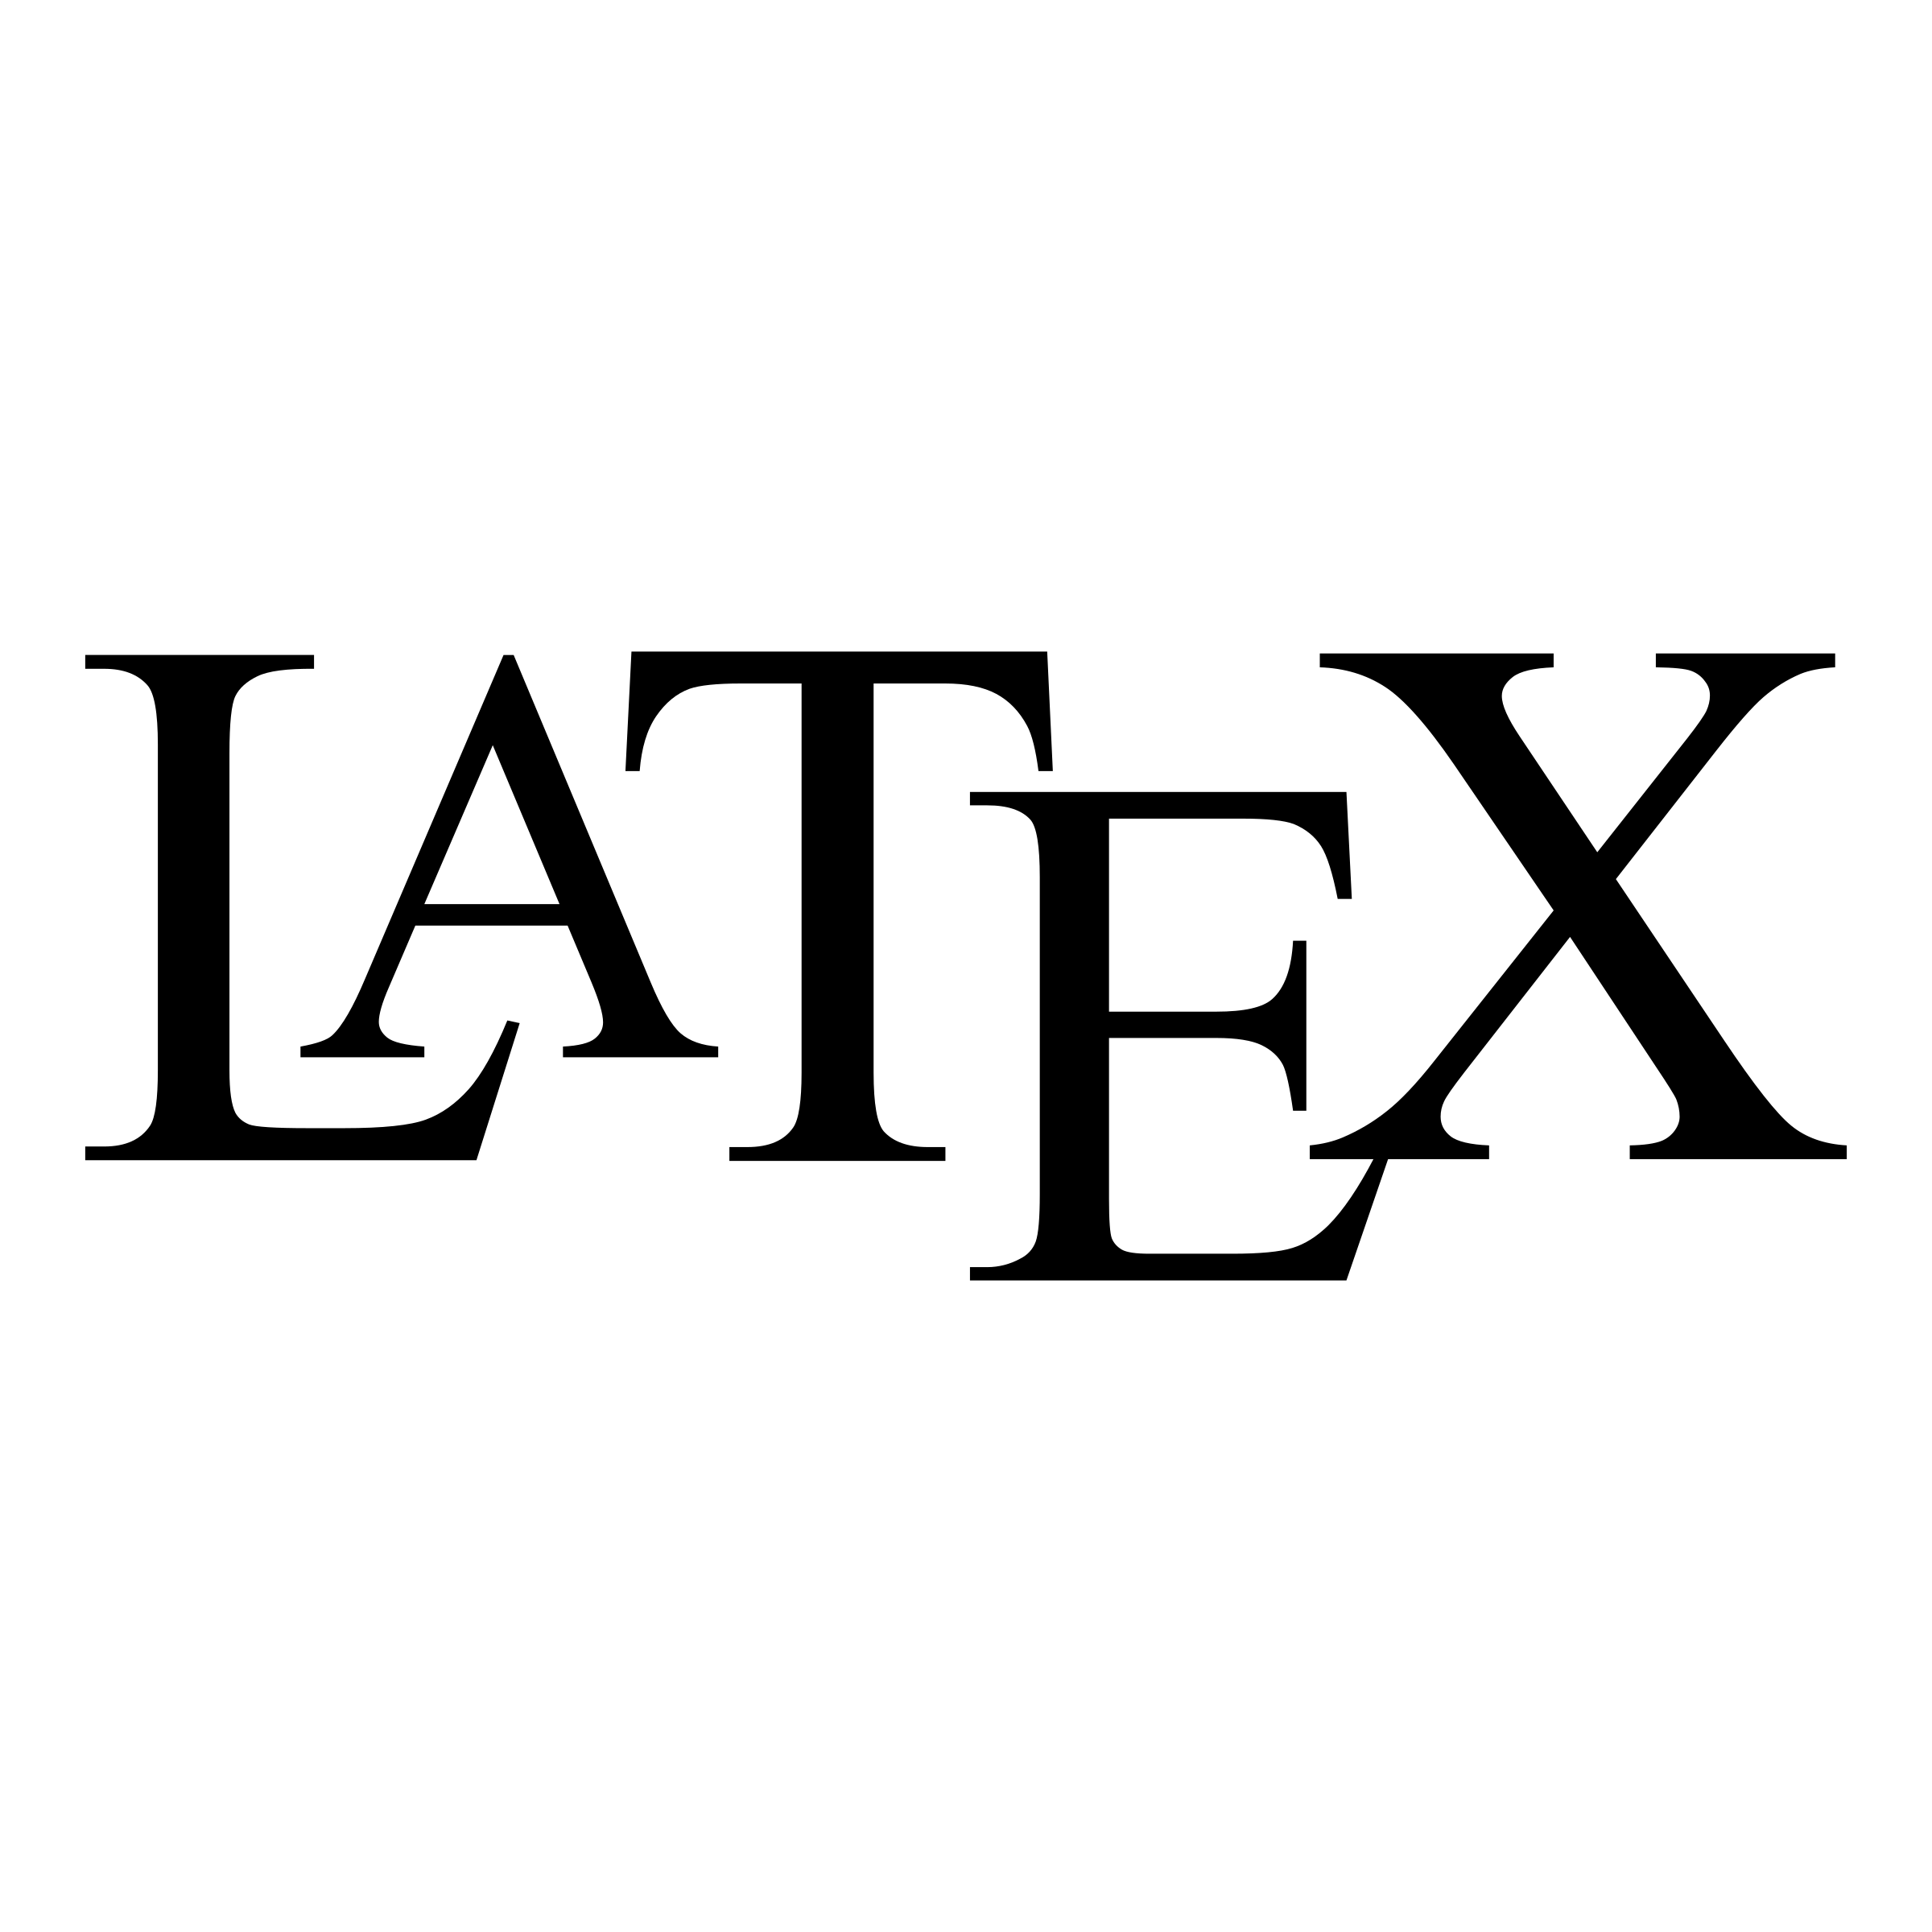
\includegraphics[scale=0.05]{LatexLogo.png}, Title Of Arounded Figure]      % must usepackage picinpar
    % bug exists
    These are the words around the figure, and the figure will appear below two lines, 
    lying in the right of the words, rather than left. The following will be fillings. 
    Hello world. Hello world. Hello world. Hello world. Hello world. Hello world. Hello world. 
    Hello world. Hello world. Hello world. Hello world. Hello world. Hello world. Hello world. 
    Hello world. Hello world. Hello world. Hello world. Hello world. Hello world. Hello world. 
    Hello world. Hello world. Hello world. Hello world. Hello world. Hello world. Hello world. 
    Hello world. Hello world. Hello world. Hello world. Hello world. Hello world. Hello world. 
    Hello world. Hello world. Hello world. Hello world. Hello world. Hello world. Hello world. 
    Hello world. Hello world. Hello world. Hello world. Hello world. Hello world. Hello world. 
    Hello world. Hello world. Hello world. Hello world. Hello world. Hello world. Hello world. 
    Hello world. Hello world. Hello world. Hello world. Hello world. Hello world. Hello world. 
    Hello world. Hello world. Hello world. Hello world. Hello world. Hello world. Hello world.
\end{figwindow}

\begin{wrapfigure}[10]{r}[1.5cm]{5cm}
    \centering
    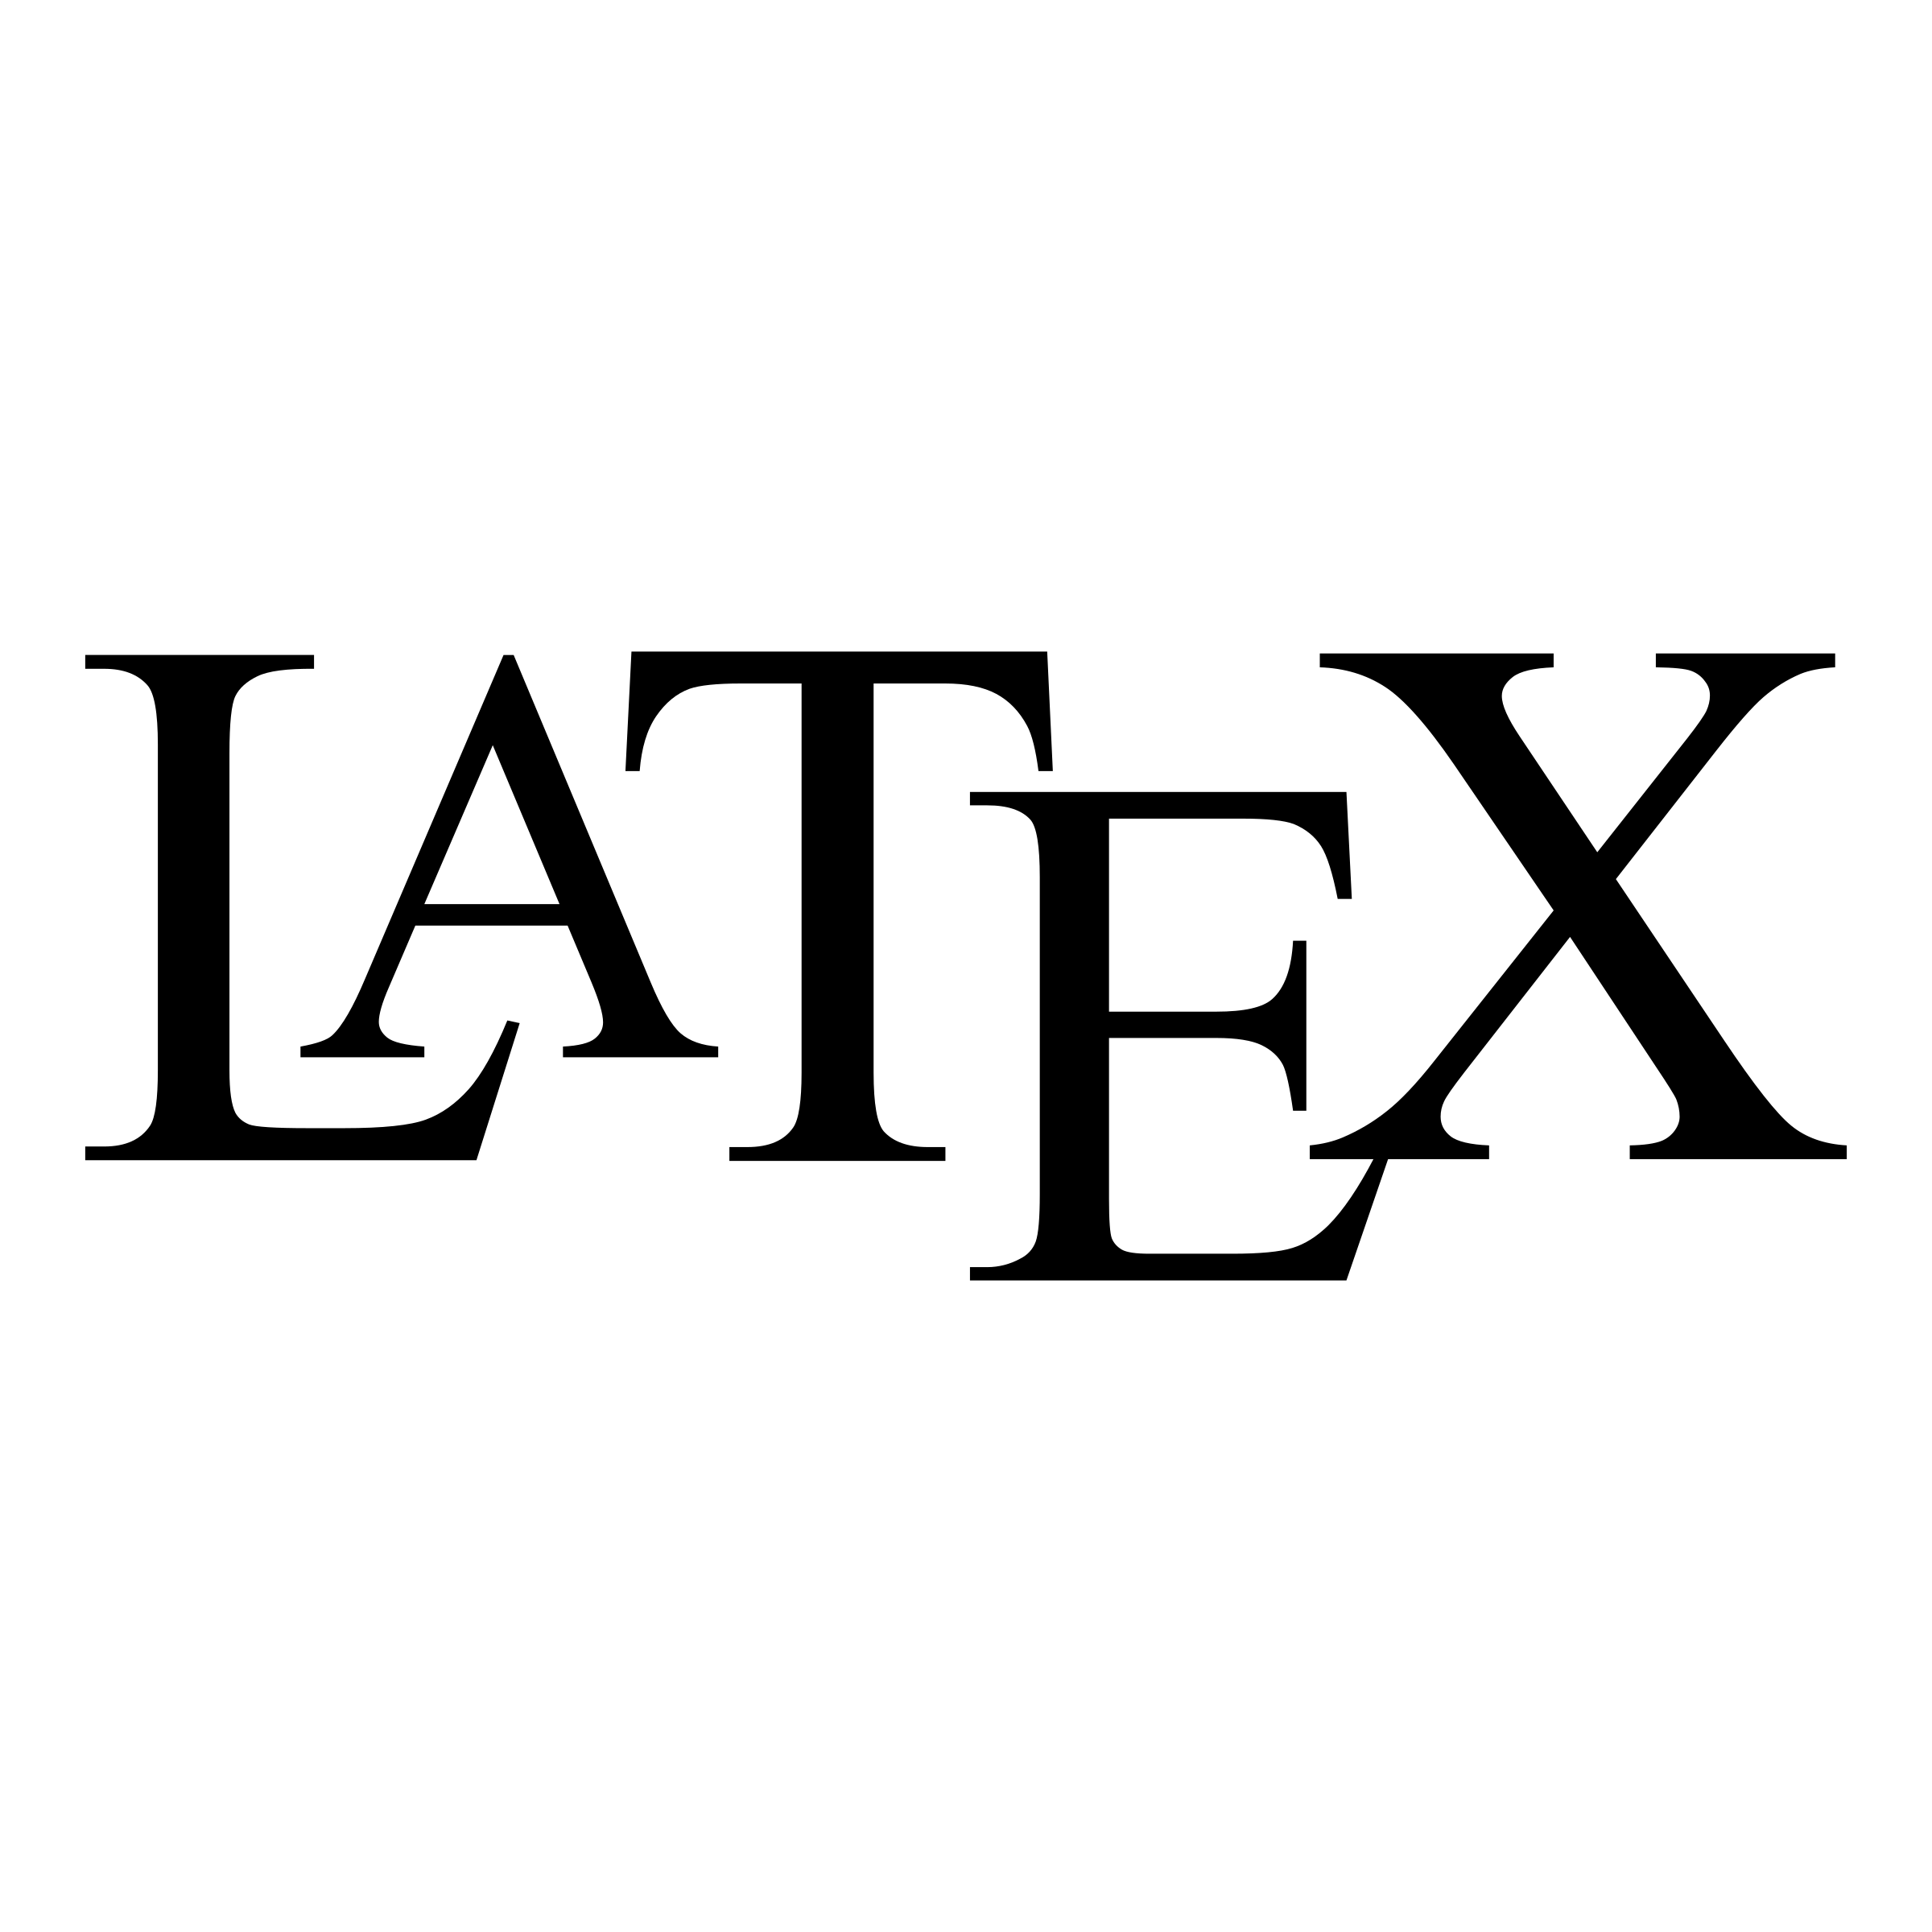
\includegraphics[scale=0.04]{LatexLogo.png}
    \caption{Title Of Arounded Figure}
\end{wrapfigure}
These are the words around the figure, and the figure will appear with height of 10 lines, 
lying in the right of the words, rather than left, and it will extend out 1.5cm, and has width of 5cm. 
The following will be fillings. 
Hello world. Hello world. Hello world. Hello world. Hello world. Hello world. Hello world. 
Hello world. Hello world. Hello world. Hello world. Hello world. Hello world. Hello world. 
Hello world. Hello world. Hello world. Hello world. Hello world. Hello world. Hello world. 
Hello world. Hello world. Hello world. Hello world. Hello world. Hello world. Hello world. 
Hello world. Hello world. Hello world. Hello world. Hello world. Hello world. Hello world. 
Hello world. Hello world. Hello world. Hello world. Hello world. Hello world. Hello world. 
Hello world. Hello world. Hello world. Hello world. Hello world. Hello world. Hello world. 
Hello world. Hello world. Hello world. Hello world. Hello world. Hello world. Hello world. 
Hello world. Hello world. Hello world. Hello world. Hello world. Hello world. Hello world. 
Hello world. Hello world. Hello world. Hello world. Hello world. Hello world. Hello world.

\subsubsection{General Float Control}
\begin{myfloat}                 % must newfloat myfloat
    \centering
    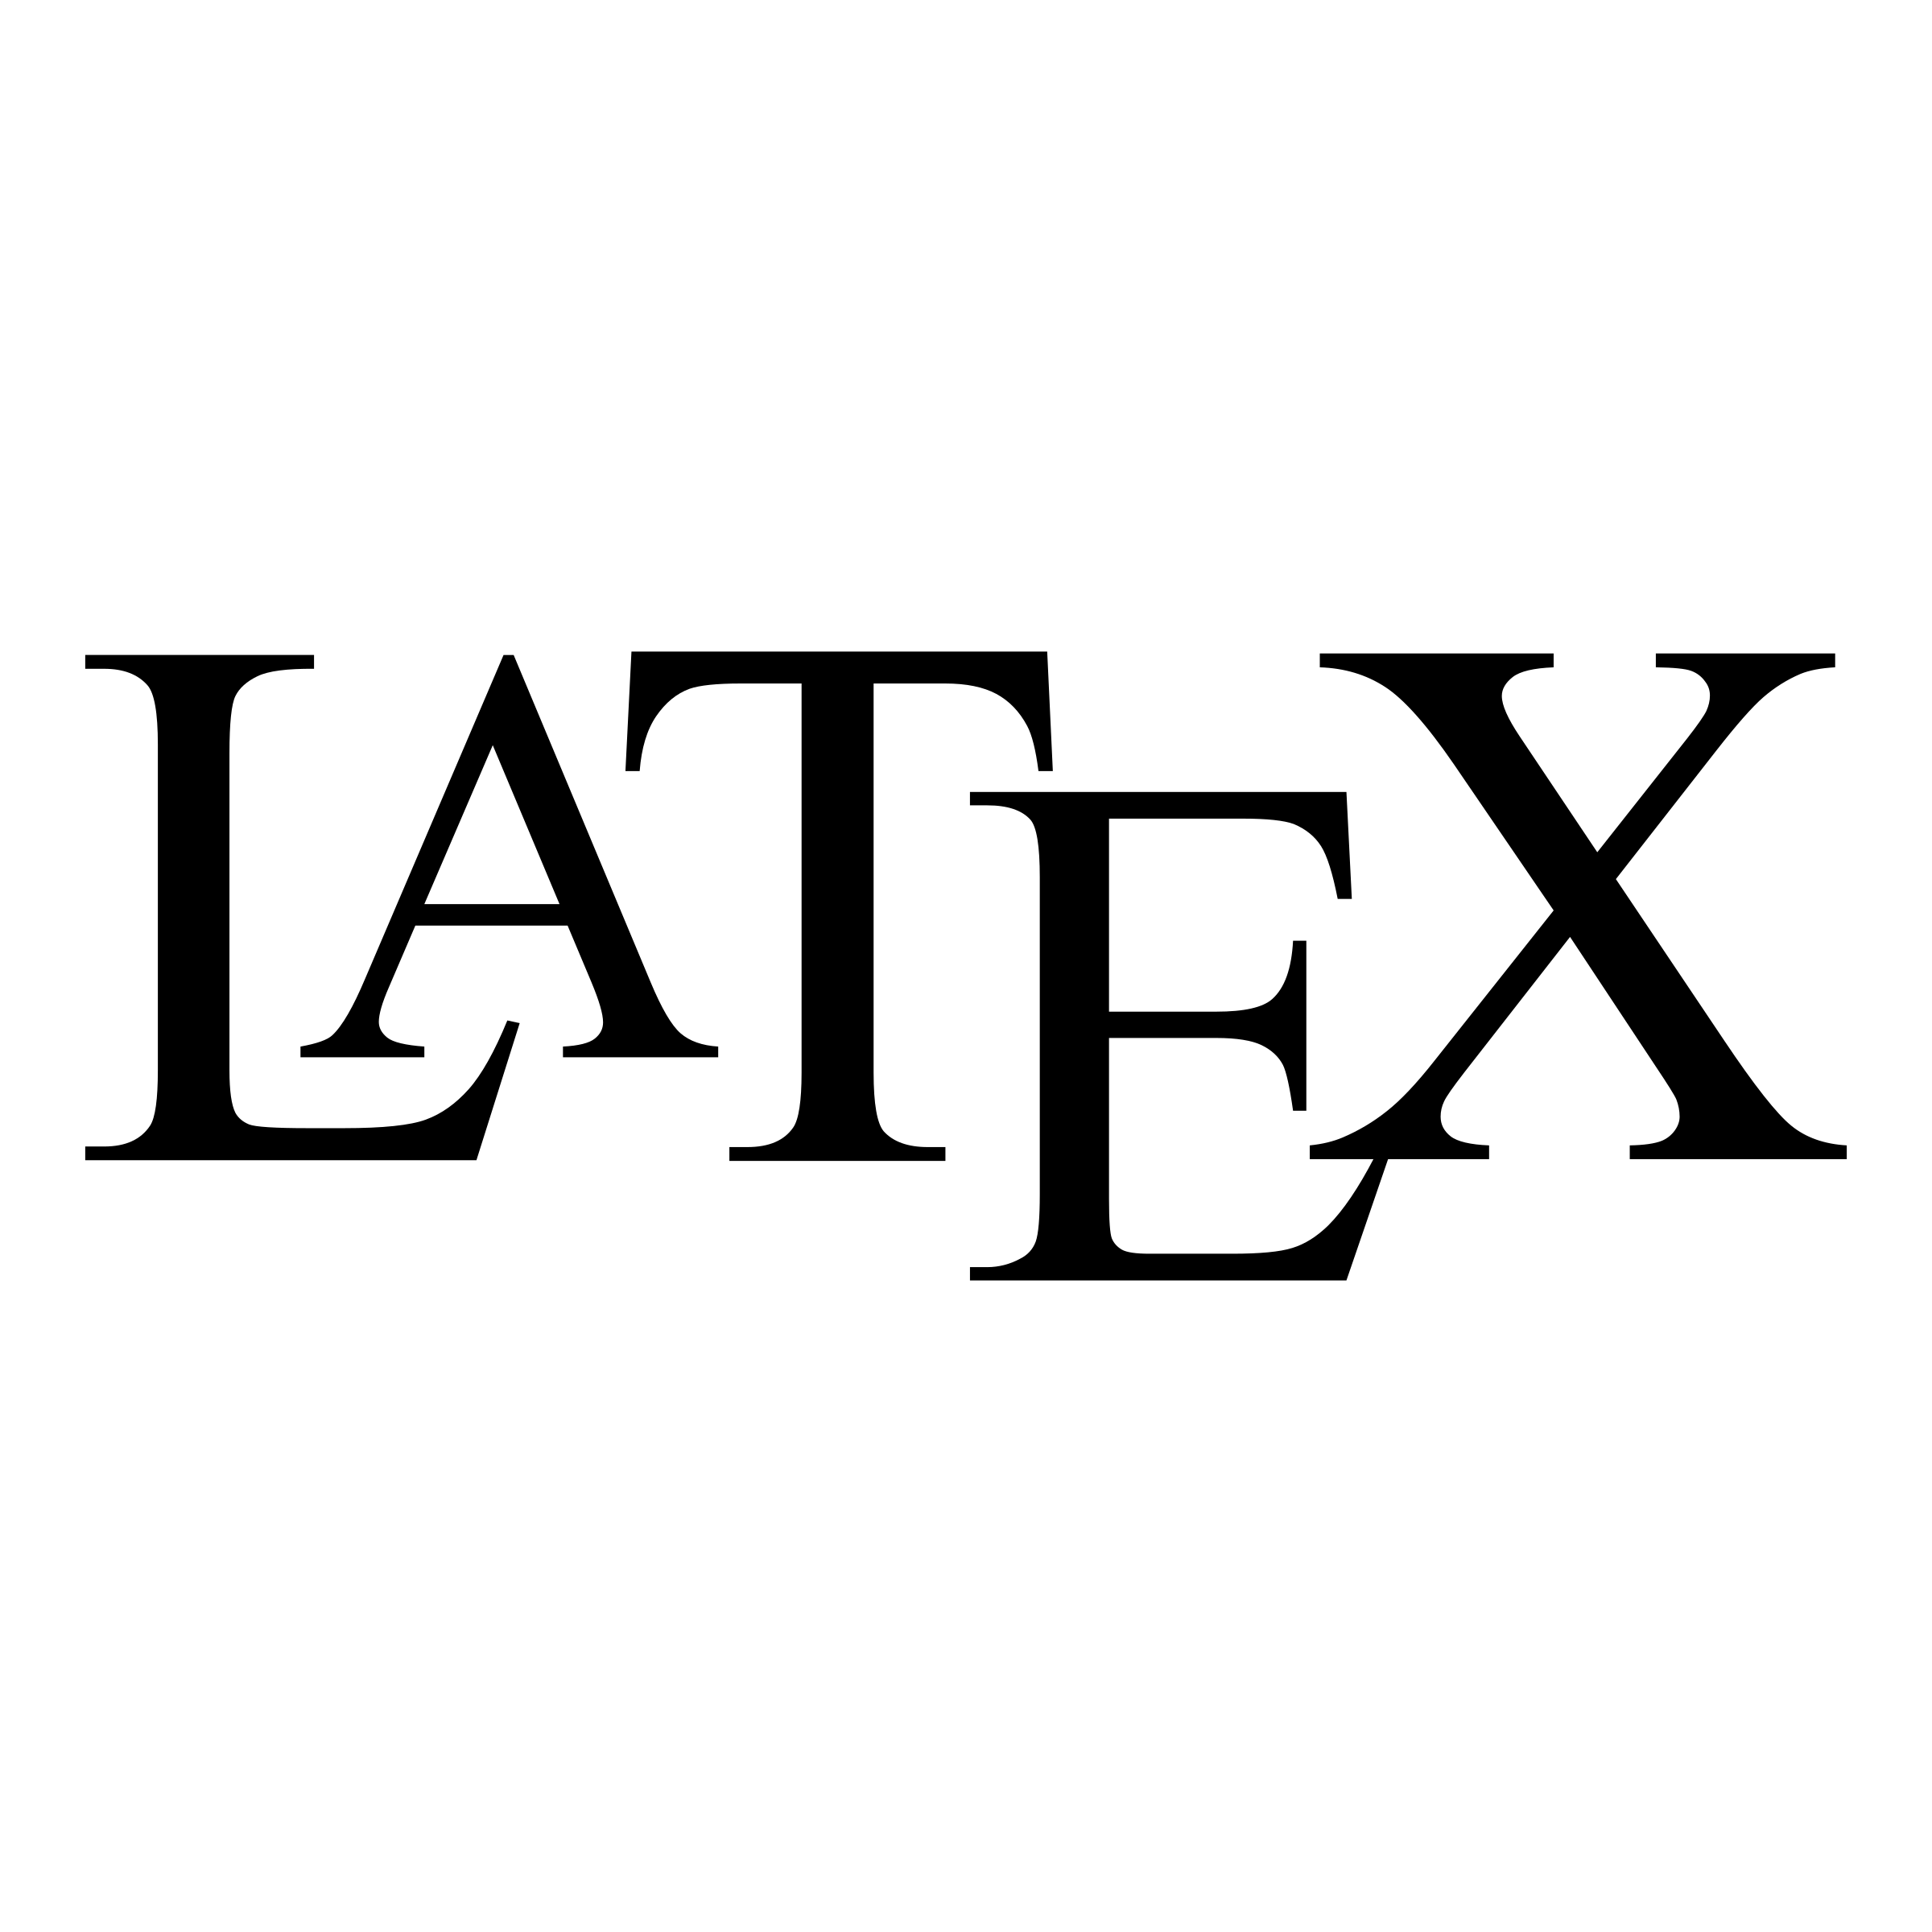
\includegraphics[scale=0.1]{LatexLogo.png}
    \caption{Figure In myfloat}
\end{myfloat}

\begin{mynewfloat}              % must DeclareFloatingEnvironment mynewfloat
    \centering
    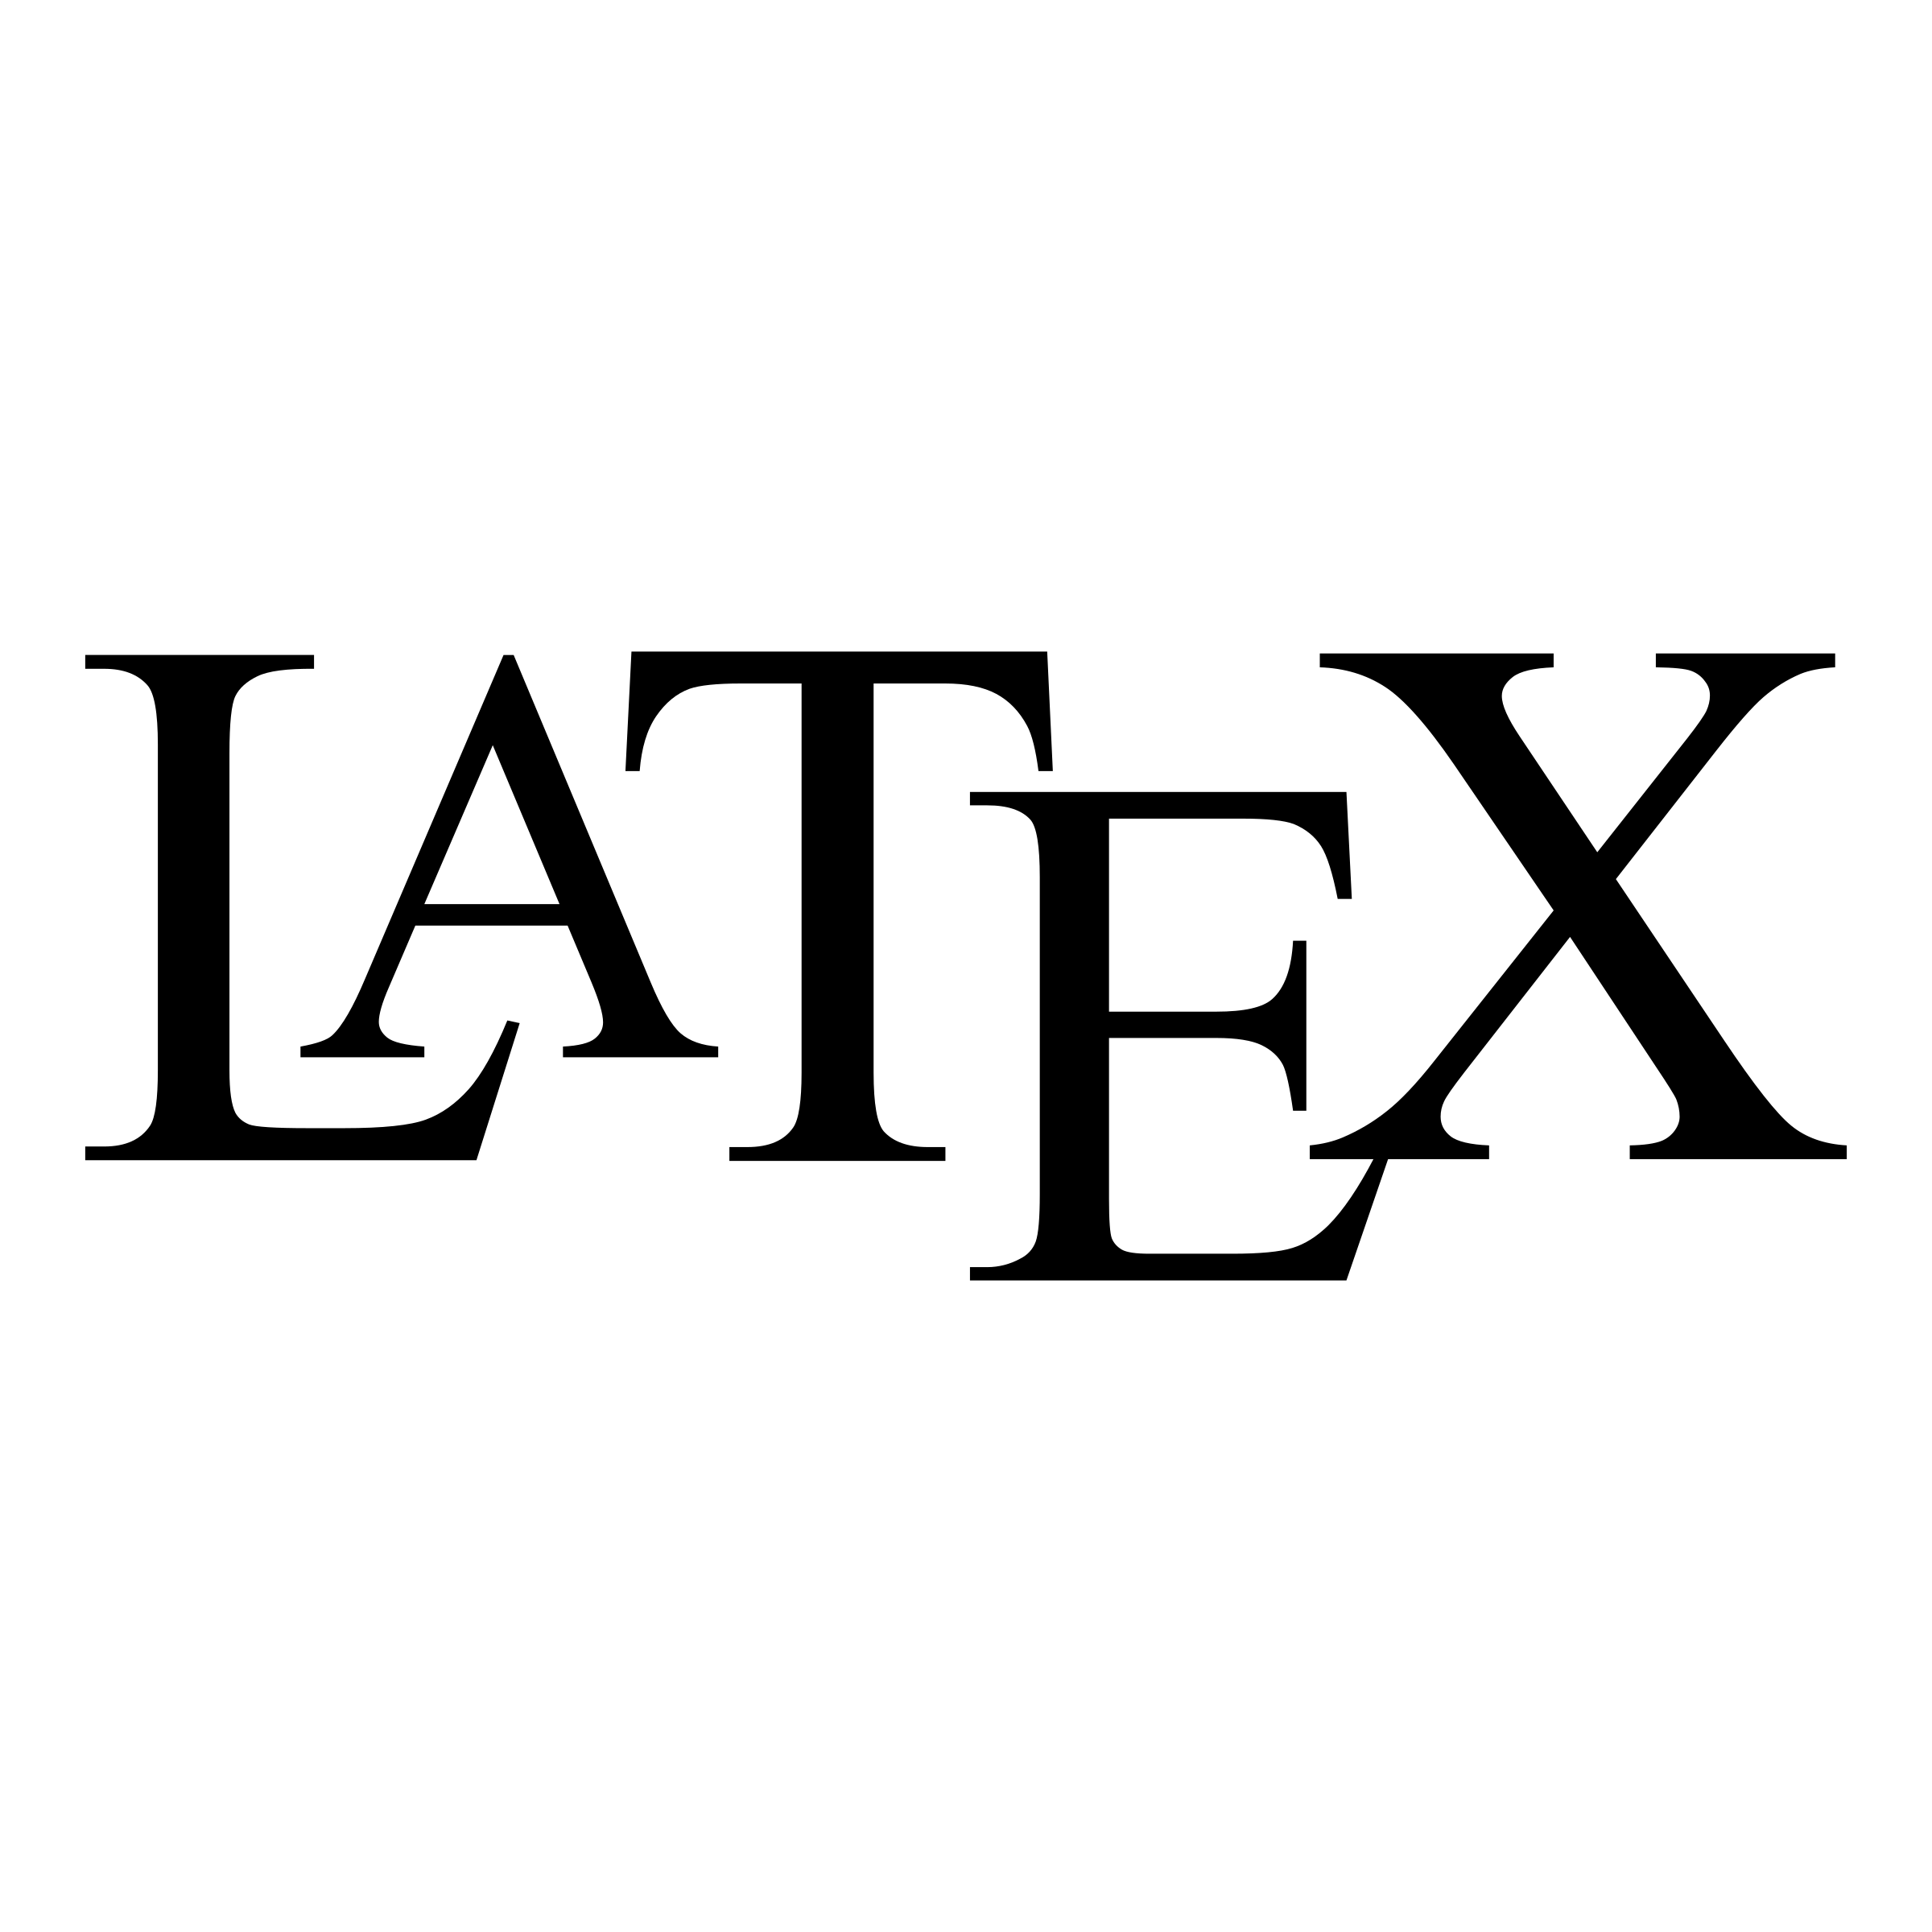
\includegraphics[scale=0.1]{LatexLogo.png}
    \caption{Figure In mynewfloat}
\end{mynewfloat}

\FloatBarrier                   % must usepackage placeins

\afterpage{\begin{figure}[H]
    \centering
    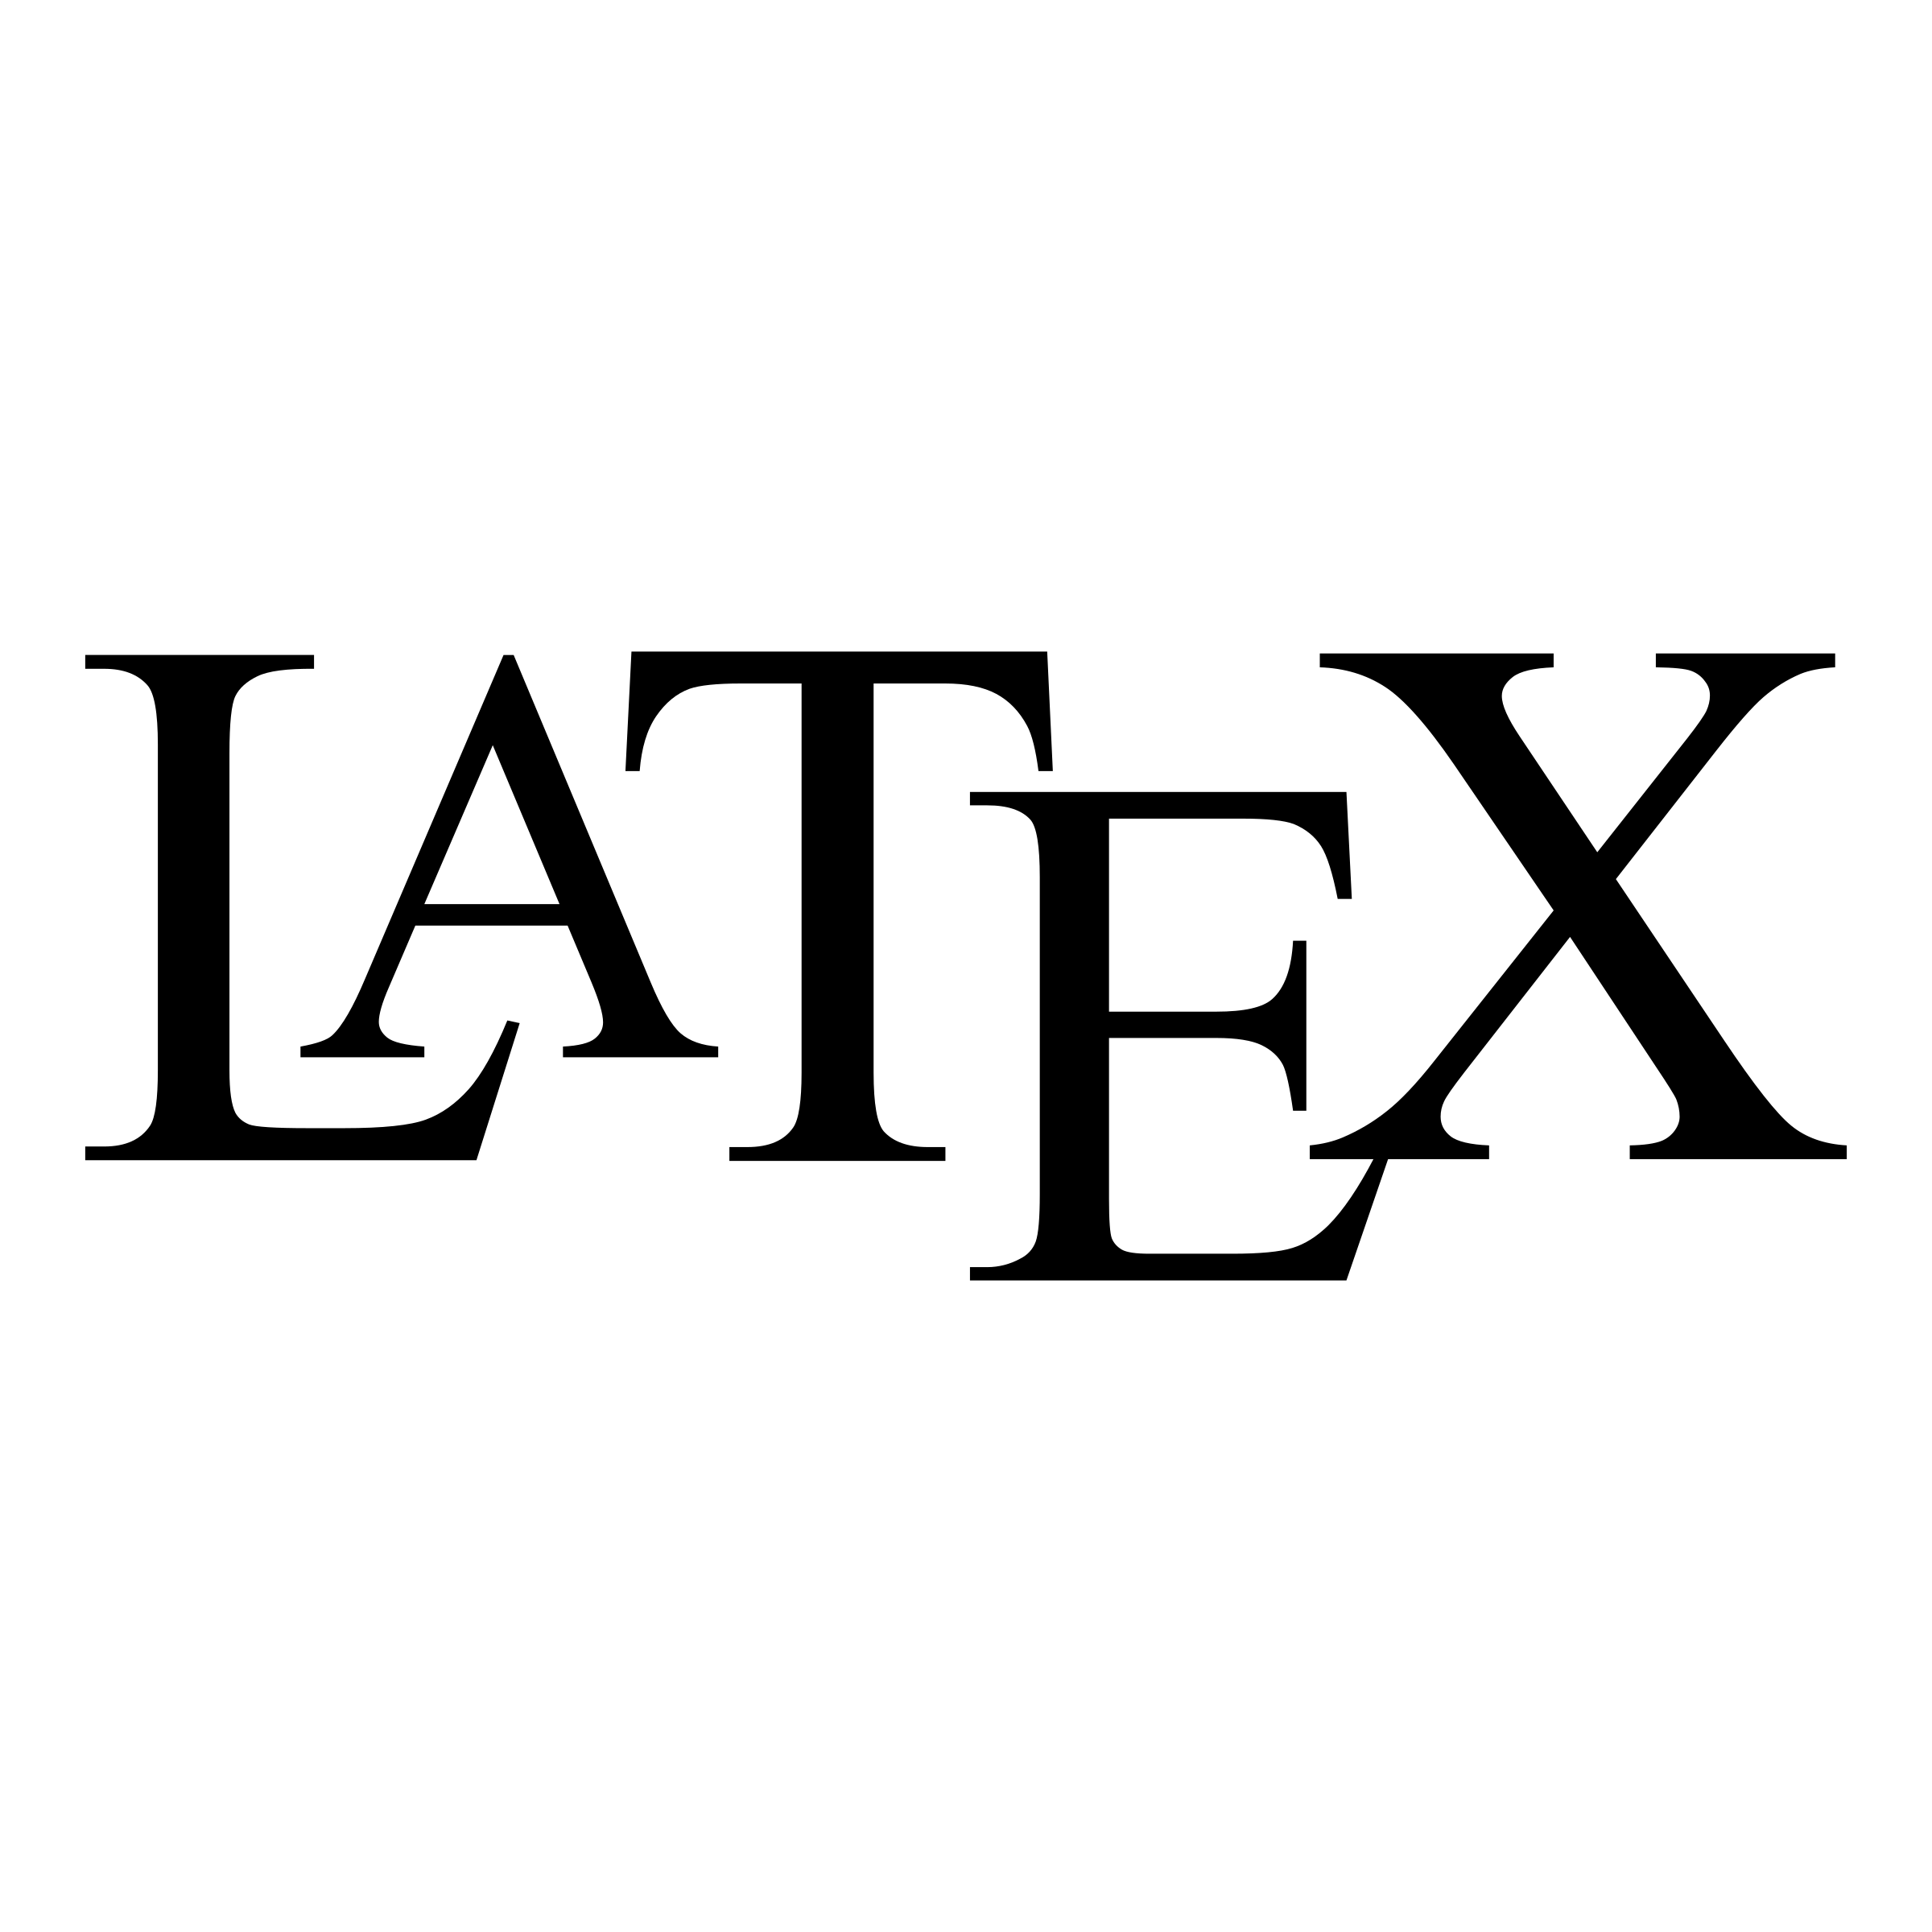
\includegraphics[scale=0.1]{LatexLogo.png}
    \caption{Figure In Top Of Next Page}
\end{figure}}

\subsection{Color}
% must usepackage xcolor
{
    \color{red}
    Red texts with \textcolor{blue}{blue words} texts.
}

% \pagecolor{cyan}

\colorbox{yellow}{Yellow box}

\fcolorbox{black}{green}{Black line green box}

\textcolor[gray]{0.5}{50\% gray text}, \textcolor[rgb]{0.6, 0.6, 0}{dark yellow text}, \textcolor[cmyk]{0.6, 0.6, 0, 0}{light purple text}

\textcolor{purple!70}{70\% purple text}, \textcolor{blue!60!black}{mixed blue and black text}, \textcolor{-red}{red complementary text}

\textcolor{darkred}{darkred text}       % must colorlet darkred

\subsection{Drawing}
\subsubsection{XY-pic}
% must usepackage xy
\begin{equation}
    \begin{gathered}
        \xymatrix{
            a & b & a+b \ar[ld]_{\alpha} \\
            1 & 2 \ar"1,1"^{\beta} & 3 \\
            \ar"1,1";"2,1"|{\gamma}
            \ar"1,2";"2,1"|\hole
        }
    \end{gathered}
\end{equation}

When $\xymatrix@1{A \ar[r]^{f} & B}$ in line text.
When $\xymatrix@1{A \ar[r]^>{f} & B}$ in line text.
When $\xymatrix@1{A \ar[r]^>>{f} & B}$ in line text.
When $\xymatrix@1{A \ar[r]^(0.6){f} & B}$ in line text.

When $\xymatrix@1{A \ar@{->}[r] & B}$ in line text.
When $\xymatrix@1{A \ar@{-->}[r] & B}$ in line text.
When $\xymatrix@1{A \ar@{=>}[r] & B}$ in line text.
When $\xymatrix@1{A \ar@{~>}[r] & B}$ in line text.
When $\xymatrix@1{A \ar@{.>}[r] & B}$ in line text.
When $\xymatrix@1{A \ar@{:>}[r] & B}$ in line text.
When $\xymatrix@1{A \ar@{-}[r] & B}$ in line text.
When $\xymatrix@1{A \ar@{}[r] & B}$ in line text.
When $\xymatrix@1{A \ar@{|->>}[r] & B}$ in line text.
When $\xymatrix@1{A \ar@{^(-_>}[r] & B}$ in line text.

When $\xymatrix@1{A \ar@/^/[r] & B}$ in line text.
When $\xymatrix@1{A \ar@/_/[r] & B}$ in line text.
When $\xymatrix@1{A \ar@(ur,dr) & B}$ in line text.

When $\xymatrix@1{A \ar@<0.5ex>[r] & \ar@<0.5ex>[l] B}$ in line text.

\begin{equation}
    \begin{gathered}
        \xymatrix@=2cm{% element separate length
            *[F]{A} \ar[r]^*+[F=]{m} & *-[o][F]{B} \\
            *[F.]{C} \ar[r]_*[F--]{n} & *[F-,]{D}
        }
    \end{gathered}
\end{equation}

\begin{equation}
    \begin{gathered}
        \xymatrix@L=1ex{% tag separate length
            \txt{Cat} \ar[r]^{f} & \txt{Dog}
        }
    \end{gathered}
\end{equation}

\begin{equation}
    \begin{gathered}
        \xymatrix@ru{% rotate
            A \ar[r] & B \ar[d] \\
            C \ar[u] & D \ar[l]
        }
    \end{gathered}
\end{equation}

\subsubsection{PSTricks}
% must usepackage pstricks or pstricks-add, bug exists
\begin{figure}[H]
    \centering
    \psset{unit=1.5cm}                                  % for setting coordinate unit
    \psset{linewidth=0.4pt}                             % for setting linewidth
    \psset{algebraic=true}                              % for using normal infix expression
    \begin{pspicture}(-3.5,-1.5)(4.5,1.5)
        \rput(-2,0){
            \psaxes[labels=none,ticks=none]{->}(0,0)(-1.2,-1.2)(1.2,1.2)
            \pscircle[linewidth=0.8pt](0,0){1}
            \pswedge[fillstyle=solid,fillcolor=gray,opacity=0.2](0,0){1}{0}{120}
            \pswedge[fillstyle=solid,fillcolor=gray,opacity=0.5](0,0){0.3}{0}{120}
            \uput[60](0.3;60){$120^{\circ}$}
            \pnode(1;120){P}
            \pnode(P|0,0){P0}
            \ncline{-}{P}{P0}
            \uput[120](P){$P$}
            \uput[d](P0){$P_0$}
        }

        \psaxes[labels=none,dx=1.57]{->}(0,0)(0,-1.2)(3.5,1.2)
        \psplot[linewidth=0.8pt]{0}{3.5}{sin(x)}
        \multido{\n=0+1.57,\i=0+90}{3}{
            \uput*[d](\n,0){\small$\i^{\circ}$}
        }
        \uput[r](*{3.5} {sin(x)}){$\sin x$}
        \pnode(!120 Pi mul 180 div 120 sin){Q}
        \pnode(Q|0,0){Q0}
        \uput[u](Q){$Q$}
        \uput[d](Q0){$Q_0$}
        \ncline{-}{Q}{Q0}

        \psline[linestyle=dashed](P)(Q)
    \end{pspicture}

    \caption{PSTricks Example}
\end{figure}

\subsubsection{TikZ}
% must usepackage tikz
\begin{figure}[H]
    \centering
    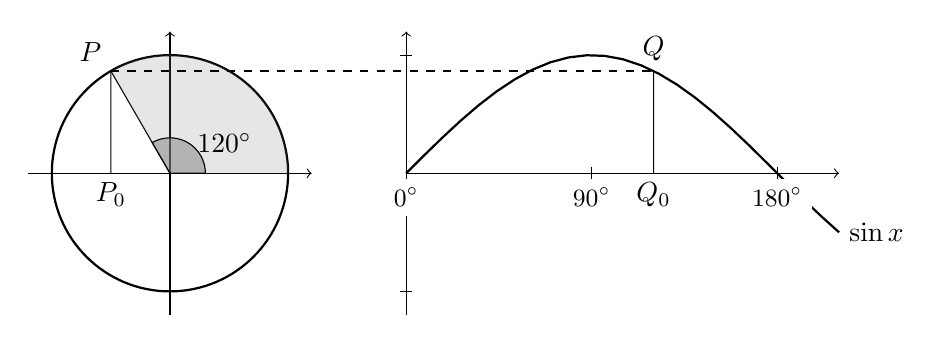
\begin{tikzpicture}[scale=1.5]
        \begin{scope}[xshift=-2cm]
            \draw[->] (-1.2,0) -- (1.2,0);
            \draw[->] (0,-1.2) -- (0,1.2);
            \draw[thick] (0,0) circle (1);
            \coordinate[label=120:$P$] (P) at (120:1);
            \coordinate[label=below:$P_0$] (P0) at (P |- 0,0);
            \draw (0,0) -- (P);
            \draw (P) -- (P0);
            \fill[fill=gray,fill opacity=0.2] (0,0) -- (0:1) arc (0:120:1) -- cycle;
            \filldraw[fill=gray, fill opacity=0.5] (0,0) -- (0:0.3) arc (0:120:0.3) -- cycle;
            \node[right] at (60:0.3) {$120^{\circ}$};
        \end{scope}

        \draw[->] (0,0) -- ({rad(210)}, 0);
        \draw[->] (0,-1.2) -- (0,1.2);
        \draw[thick,domain=0:rad(210)] plot (\x, {sin(\x r)}) node[right] {$\sin x$};
        \foreach \t in {0, 90, 180} {
            \draw ({rad(\t)}, -0.05) -- ({rad(\t)}, 0.05);
            \node[below, outer sep=2pt, fill=white, font=\small] at ({rad(\t)}, 0) {$\t^{\circ}$};
        }
        \foreach \y in {-1,1} {
            \draw (-0.05,\y) -- (0.05,\y);
        }
        \coordinate[label=above:$Q$] (Q) at ({rad(120)}, {sin(120)});
        \coordinate[label=below:$Q_0$] (Q0) at (Q |- 0,0);
        \draw (Q) -- (Q0);
        \draw[dashed] (P) -- (Q);
    \end{tikzpicture}

    \caption{TikZ Example}
\end{figure}